
\documentclass{article} % For LaTeX2e
\usepackage{iclr2027_conference,times}
\usepackage{graphicx}
\usepackage{subcaption}
\usepackage{booktabs}
\usepackage{multirow}

% Optional math commands from https://github.com/goodfeli/dlbook_notation.
%%%%% NEW MATH DEFINITIONS %%%%%

\usepackage{amsmath,amsfonts,bm}

% Mark sections of captions for referring to divisions of figures
\newcommand{\figleft}{{\em (Left)}}
\newcommand{\figcenter}{{\em (Center)}}
\newcommand{\figright}{{\em (Right)}}
\newcommand{\figtop}{{\em (Top)}}
\newcommand{\figbottom}{{\em (Bottom)}}
\newcommand{\captiona}{{\em (a)}}
\newcommand{\captionb}{{\em (b)}}
\newcommand{\captionc}{{\em (c)}}
\newcommand{\captiond}{{\em (d)}}

% Highlight a newly defined term
\newcommand{\newterm}[1]{{\bf #1}}


% Figure reference, lower-case.
\def\figref#1{figure~\ref{#1}}
% Figure reference, capital. For start of sentence
\def\Figref#1{Figure~\ref{#1}}
\def\twofigref#1#2{figures \ref{#1} and \ref{#2}}
\def\quadfigref#1#2#3#4{figures \ref{#1}, \ref{#2}, \ref{#3} and \ref{#4}}
% Section reference, lower-case.
\def\secref#1{section~\ref{#1}}
% Section reference, capital.
\def\Secref#1{Section~\ref{#1}}
% Reference to two sections.
\def\twosecrefs#1#2{sections \ref{#1} and \ref{#2}}
% Reference to three sections.
\def\secrefs#1#2#3{sections \ref{#1}, \ref{#2} and \ref{#3}}
% Reference to an equation, lower-case.
\def\eqref#1{equation~\ref{#1}}
% Reference to an equation, upper case
\def\Eqref#1{Equation~\ref{#1}}
% A raw reference to an equation---avoid using if possible
\def\plaineqref#1{\ref{#1}}
% Reference to a chapter, lower-case.
\def\chapref#1{chapter~\ref{#1}}
% Reference to an equation, upper case.
\def\Chapref#1{Chapter~\ref{#1}}
% Reference to a range of chapters
\def\rangechapref#1#2{chapters\ref{#1}--\ref{#2}}
% Reference to an algorithm, lower-case.
\def\algref#1{algorithm~\ref{#1}}
% Reference to an algorithm, upper case.
\def\Algref#1{Algorithm~\ref{#1}}
\def\twoalgref#1#2{algorithms \ref{#1} and \ref{#2}}
\def\Twoalgref#1#2{Algorithms \ref{#1} and \ref{#2}}
% Reference to a part, lower case
\def\partref#1{part~\ref{#1}}
% Reference to a part, upper case
\def\Partref#1{Part~\ref{#1}}
\def\twopartref#1#2{parts \ref{#1} and \ref{#2}}

\def\ceil#1{\lceil #1 \rceil}
\def\floor#1{\lfloor #1 \rfloor}
\def\1{\bm{1}}
\newcommand{\train}{\mathcal{D}}
\newcommand{\valid}{\mathcal{D_{\mathrm{valid}}}}
\newcommand{\test}{\mathcal{D_{\mathrm{test}}}}

\def\eps{{\epsilon}}


% Random variables
\def\reta{{\textnormal{$\eta$}}}
\def\ra{{\textnormal{a}}}
\def\rb{{\textnormal{b}}}
\def\rc{{\textnormal{c}}}
\def\rd{{\textnormal{d}}}
\def\re{{\textnormal{e}}}
\def\rf{{\textnormal{f}}}
\def\rg{{\textnormal{g}}}
\def\rh{{\textnormal{h}}}
\def\ri{{\textnormal{i}}}
\def\rj{{\textnormal{j}}}
\def\rk{{\textnormal{k}}}
\def\rl{{\textnormal{l}}}
% rm is already a command, just don't name any random variables m
\def\rn{{\textnormal{n}}}
\def\ro{{\textnormal{o}}}
\def\rp{{\textnormal{p}}}
\def\rq{{\textnormal{q}}}
\def\rr{{\textnormal{r}}}
\def\rs{{\textnormal{s}}}
\def\rt{{\textnormal{t}}}
\def\ru{{\textnormal{u}}}
\def\rv{{\textnormal{v}}}
\def\rw{{\textnormal{w}}}
\def\rx{{\textnormal{x}}}
\def\ry{{\textnormal{y}}}
\def\rz{{\textnormal{z}}}

% Random vectors
\def\rvepsilon{{\mathbf{\epsilon}}}
\def\rvtheta{{\mathbf{\theta}}}
\def\rva{{\mathbf{a}}}
\def\rvb{{\mathbf{b}}}
\def\rvc{{\mathbf{c}}}
\def\rvd{{\mathbf{d}}}
\def\rve{{\mathbf{e}}}
\def\rvf{{\mathbf{f}}}
\def\rvg{{\mathbf{g}}}
\def\rvh{{\mathbf{h}}}
\def\rvu{{\mathbf{i}}}
\def\rvj{{\mathbf{j}}}
\def\rvk{{\mathbf{k}}}
\def\rvl{{\mathbf{l}}}
\def\rvm{{\mathbf{m}}}
\def\rvn{{\mathbf{n}}}
\def\rvo{{\mathbf{o}}}
\def\rvp{{\mathbf{p}}}
\def\rvq{{\mathbf{q}}}
\def\rvr{{\mathbf{r}}}
\def\rvs{{\mathbf{s}}}
\def\rvt{{\mathbf{t}}}
\def\rvu{{\mathbf{u}}}
\def\rvv{{\mathbf{v}}}
\def\rvw{{\mathbf{w}}}
\def\rvx{{\mathbf{x}}}
\def\rvy{{\mathbf{y}}}
\def\rvz{{\mathbf{z}}}

% Elements of random vectors
\def\erva{{\textnormal{a}}}
\def\ervb{{\textnormal{b}}}
\def\ervc{{\textnormal{c}}}
\def\ervd{{\textnormal{d}}}
\def\erve{{\textnormal{e}}}
\def\ervf{{\textnormal{f}}}
\def\ervg{{\textnormal{g}}}
\def\ervh{{\textnormal{h}}}
\def\ervi{{\textnormal{i}}}
\def\ervj{{\textnormal{j}}}
\def\ervk{{\textnormal{k}}}
\def\ervl{{\textnormal{l}}}
\def\ervm{{\textnormal{m}}}
\def\ervn{{\textnormal{n}}}
\def\ervo{{\textnormal{o}}}
\def\ervp{{\textnormal{p}}}
\def\ervq{{\textnormal{q}}}
\def\ervr{{\textnormal{r}}}
\def\ervs{{\textnormal{s}}}
\def\ervt{{\textnormal{t}}}
\def\ervu{{\textnormal{u}}}
\def\ervv{{\textnormal{v}}}
\def\ervw{{\textnormal{w}}}
\def\ervx{{\textnormal{x}}}
\def\ervy{{\textnormal{y}}}
\def\ervz{{\textnormal{z}}}

% Random matrices
\def\rmA{{\mathbf{A}}}
\def\rmB{{\mathbf{B}}}
\def\rmC{{\mathbf{C}}}
\def\rmD{{\mathbf{D}}}
\def\rmE{{\mathbf{E}}}
\def\rmF{{\mathbf{F}}}
\def\rmG{{\mathbf{G}}}
\def\rmH{{\mathbf{H}}}
\def\rmI{{\mathbf{I}}}
\def\rmJ{{\mathbf{J}}}
\def\rmK{{\mathbf{K}}}
\def\rmL{{\mathbf{L}}}
\def\rmM{{\mathbf{M}}}
\def\rmN{{\mathbf{N}}}
\def\rmO{{\mathbf{O}}}
\def\rmP{{\mathbf{P}}}
\def\rmQ{{\mathbf{Q}}}
\def\rmR{{\mathbf{R}}}
\def\rmS{{\mathbf{S}}}
\def\rmT{{\mathbf{T}}}
\def\rmU{{\mathbf{U}}}
\def\rmV{{\mathbf{V}}}
\def\rmW{{\mathbf{W}}}
\def\rmX{{\mathbf{X}}}
\def\rmY{{\mathbf{Y}}}
\def\rmZ{{\mathbf{Z}}}

% Elements of random matrices
\def\ermA{{\textnormal{A}}}
\def\ermB{{\textnormal{B}}}
\def\ermC{{\textnormal{C}}}
\def\ermD{{\textnormal{D}}}
\def\ermE{{\textnormal{E}}}
\def\ermF{{\textnormal{F}}}
\def\ermG{{\textnormal{G}}}
\def\ermH{{\textnormal{H}}}
\def\ermI{{\textnormal{I}}}
\def\ermJ{{\textnormal{J}}}
\def\ermK{{\textnormal{K}}}
\def\ermL{{\textnormal{L}}}
\def\ermM{{\textnormal{M}}}
\def\ermN{{\textnormal{N}}}
\def\ermO{{\textnormal{O}}}
\def\ermP{{\textnormal{P}}}
\def\ermQ{{\textnormal{Q}}}
\def\ermR{{\textnormal{R}}}
\def\ermS{{\textnormal{S}}}
\def\ermT{{\textnormal{T}}}
\def\ermU{{\textnormal{U}}}
\def\ermV{{\textnormal{V}}}
\def\ermW{{\textnormal{W}}}
\def\ermX{{\textnormal{X}}}
\def\ermY{{\textnormal{Y}}}
\def\ermZ{{\textnormal{Z}}}

% Vectors
\def\vzero{{\bm{0}}}
\def\vone{{\bm{1}}}
\def\vmu{{\bm{\mu}}}
\def\vtheta{{\bm{\theta}}}
\def\va{{\bm{a}}}
\def\vb{{\bm{b}}}
\def\vc{{\bm{c}}}
\def\vd{{\bm{d}}}
\def\ve{{\bm{e}}}
\def\vf{{\bm{f}}}
\def\vg{{\bm{g}}}
\def\vh{{\bm{h}}}
\def\vi{{\bm{i}}}
\def\vj{{\bm{j}}}
\def\vk{{\bm{k}}}
\def\vl{{\bm{l}}}
\def\vm{{\bm{m}}}
\def\vn{{\bm{n}}}
\def\vo{{\bm{o}}}
\def\vp{{\bm{p}}}
\def\vq{{\bm{q}}}
\def\vr{{\bm{r}}}
\def\vs{{\bm{s}}}
\def\vt{{\bm{t}}}
\def\vu{{\bm{u}}}
\def\vv{{\bm{v}}}
\def\vw{{\bm{w}}}
\def\vx{{\bm{x}}}
\def\vy{{\bm{y}}}
\def\vz{{\bm{z}}}

% Elements of vectors
\def\evalpha{{\alpha}}
\def\evbeta{{\beta}}
\def\evepsilon{{\epsilon}}
\def\evlambda{{\lambda}}
\def\evomega{{\omega}}
\def\evmu{{\mu}}
\def\evpsi{{\psi}}
\def\evsigma{{\sigma}}
\def\evtheta{{\theta}}
\def\eva{{a}}
\def\evb{{b}}
\def\evc{{c}}
\def\evd{{d}}
\def\eve{{e}}
\def\evf{{f}}
\def\evg{{g}}
\def\evh{{h}}
\def\evi{{i}}
\def\evj{{j}}
\def\evk{{k}}
\def\evl{{l}}
\def\evm{{m}}
\def\evn{{n}}
\def\evo{{o}}
\def\evp{{p}}
\def\evq{{q}}
\def\evr{{r}}
\def\evs{{s}}
\def\evt{{t}}
\def\evu{{u}}
\def\evv{{v}}
\def\evw{{w}}
\def\evx{{x}}
\def\evy{{y}}
\def\evz{{z}}

% Matrix
\def\mA{{\bm{A}}}
\def\mB{{\bm{B}}}
\def\mC{{\bm{C}}}
\def\mD{{\bm{D}}}
\def\mE{{\bm{E}}}
\def\mF{{\bm{F}}}
\def\mG{{\bm{G}}}
\def\mH{{\bm{H}}}
\def\mI{{\bm{I}}}
\def\mJ{{\bm{J}}}
\def\mK{{\bm{K}}}
\def\mL{{\bm{L}}}
\def\mM{{\bm{M}}}
\def\mN{{\bm{N}}}
\def\mO{{\bm{O}}}
\def\mP{{\bm{P}}}
\def\mQ{{\bm{Q}}}
\def\mR{{\bm{R}}}
\def\mS{{\bm{S}}}
\def\mT{{\bm{T}}}
\def\mU{{\bm{U}}}
\def\mV{{\bm{V}}}
\def\mW{{\bm{W}}}
\def\mX{{\bm{X}}}
\def\mY{{\bm{Y}}}
\def\mZ{{\bm{Z}}}
\def\mBeta{{\bm{\beta}}}
\def\mPhi{{\bm{\Phi}}}
\def\mLambda{{\bm{\Lambda}}}
\def\mSigma{{\bm{\Sigma}}}

% Tensor
\DeclareMathAlphabet{\mathsfit}{\encodingdefault}{\sfdefault}{m}{sl}
\SetMathAlphabet{\mathsfit}{bold}{\encodingdefault}{\sfdefault}{bx}{n}
\newcommand{\tens}[1]{\bm{\mathsfit{#1}}}
\def\tA{{\tens{A}}}
\def\tB{{\tens{B}}}
\def\tC{{\tens{C}}}
\def\tD{{\tens{D}}}
\def\tE{{\tens{E}}}
\def\tF{{\tens{F}}}
\def\tG{{\tens{G}}}
\def\tH{{\tens{H}}}
\def\tI{{\tens{I}}}
\def\tJ{{\tens{J}}}
\def\tK{{\tens{K}}}
\def\tL{{\tens{L}}}
\def\tM{{\tens{M}}}
\def\tN{{\tens{N}}}
\def\tO{{\tens{O}}}
\def\tP{{\tens{P}}}
\def\tQ{{\tens{Q}}}
\def\tR{{\tens{R}}}
\def\tS{{\tens{S}}}
\def\tT{{\tens{T}}}
\def\tU{{\tens{U}}}
\def\tV{{\tens{V}}}
\def\tW{{\tens{W}}}
\def\tX{{\tens{X}}}
\def\tY{{\tens{Y}}}
\def\tZ{{\tens{Z}}}


% Graph
\def\gA{{\mathcal{A}}}
\def\gB{{\mathcal{B}}}
\def\gC{{\mathcal{C}}}
\def\gD{{\mathcal{D}}}
\def\gE{{\mathcal{E}}}
\def\gF{{\mathcal{F}}}
\def\gG{{\mathcal{G}}}
\def\gH{{\mathcal{H}}}
\def\gI{{\mathcal{I}}}
\def\gJ{{\mathcal{J}}}
\def\gK{{\mathcal{K}}}
\def\gL{{\mathcal{L}}}
\def\gM{{\mathcal{M}}}
\def\gN{{\mathcal{N}}}
\def\gO{{\mathcal{O}}}
\def\gP{{\mathcal{P}}}
\def\gQ{{\mathcal{Q}}}
\def\gR{{\mathcal{R}}}
\def\gS{{\mathcal{S}}}
\def\gT{{\mathcal{T}}}
\def\gU{{\mathcal{U}}}
\def\gV{{\mathcal{V}}}
\def\gW{{\mathcal{W}}}
\def\gX{{\mathcal{X}}}
\def\gY{{\mathcal{Y}}}
\def\gZ{{\mathcal{Z}}}

% Sets
\def\sA{{\mathbb{A}}}
\def\sB{{\mathbb{B}}}
\def\sC{{\mathbb{C}}}
\def\sD{{\mathbb{D}}}
% Don't use a set called E, because this would be the same as our symbol
% for expectation.
\def\sF{{\mathbb{F}}}
\def\sG{{\mathbb{G}}}
\def\sH{{\mathbb{H}}}
\def\sI{{\mathbb{I}}}
\def\sJ{{\mathbb{J}}}
\def\sK{{\mathbb{K}}}
\def\sL{{\mathbb{L}}}
\def\sM{{\mathbb{M}}}
\def\sN{{\mathbb{N}}}
\def\sO{{\mathbb{O}}}
\def\sP{{\mathbb{P}}}
\def\sQ{{\mathbb{Q}}}
\def\sR{{\mathbb{R}}}
\def\sS{{\mathbb{S}}}
\def\sT{{\mathbb{T}}}
\def\sU{{\mathbb{U}}}
\def\sV{{\mathbb{V}}}
\def\sW{{\mathbb{W}}}
\def\sX{{\mathbb{X}}}
\def\sY{{\mathbb{Y}}}
\def\sZ{{\mathbb{Z}}}

% Entries of a matrix
\def\emLambda{{\Lambda}}
\def\emA{{A}}
\def\emB{{B}}
\def\emC{{C}}
\def\emD{{D}}
\def\emE{{E}}
\def\emF{{F}}
\def\emG{{G}}
\def\emH{{H}}
\def\emI{{I}}
\def\emJ{{J}}
\def\emK{{K}}
\def\emL{{L}}
\def\emM{{M}}
\def\emN{{N}}
\def\emO{{O}}
\def\emP{{P}}
\def\emQ{{Q}}
\def\emR{{R}}
\def\emS{{S}}
\def\emT{{T}}
\def\emU{{U}}
\def\emV{{V}}
\def\emW{{W}}
\def\emX{{X}}
\def\emY{{Y}}
\def\emZ{{Z}}
\def\emSigma{{\Sigma}}

% entries of a tensor
% Same font as tensor, without \bm wrapper
\newcommand{\etens}[1]{\mathsfit{#1}}
\def\etLambda{{\etens{\Lambda}}}
\def\etA{{\etens{A}}}
\def\etB{{\etens{B}}}
\def\etC{{\etens{C}}}
\def\etD{{\etens{D}}}
\def\etE{{\etens{E}}}
\def\etF{{\etens{F}}}
\def\etG{{\etens{G}}}
\def\etH{{\etens{H}}}
\def\etI{{\etens{I}}}
\def\etJ{{\etens{J}}}
\def\etK{{\etens{K}}}
\def\etL{{\etens{L}}}
\def\etM{{\etens{M}}}
\def\etN{{\etens{N}}}
\def\etO{{\etens{O}}}
\def\etP{{\etens{P}}}
\def\etQ{{\etens{Q}}}
\def\etR{{\etens{R}}}
\def\etS{{\etens{S}}}
\def\etT{{\etens{T}}}
\def\etU{{\etens{U}}}
\def\etV{{\etens{V}}}
\def\etW{{\etens{W}}}
\def\etX{{\etens{X}}}
\def\etY{{\etens{Y}}}
\def\etZ{{\etens{Z}}}

% The true underlying data generating distribution
\newcommand{\pdata}{p_{\rm{data}}}
% The empirical distribution defined by the training set
\newcommand{\ptrain}{\hat{p}_{\rm{data}}}
\newcommand{\Ptrain}{\hat{P}_{\rm{data}}}
% The model distribution
\newcommand{\pmodel}{p_{\rm{model}}}
\newcommand{\Pmodel}{P_{\rm{model}}}
\newcommand{\ptildemodel}{\tilde{p}_{\rm{model}}}
% Stochastic autoencoder distributions
\newcommand{\pencode}{p_{\rm{encoder}}}
\newcommand{\pdecode}{p_{\rm{decoder}}}
\newcommand{\precons}{p_{\rm{reconstruct}}}

\newcommand{\laplace}{\mathrm{Laplace}} % Laplace distribution

\newcommand{\E}{\mathbb{E}}
\newcommand{\Ls}{\mathcal{L}}
\newcommand{\R}{\mathbb{R}}
\newcommand{\emp}{\tilde{p}}
\newcommand{\lr}{\alpha}
\newcommand{\reg}{\lambda}
\newcommand{\rect}{\mathrm{rectifier}}
\newcommand{\softmax}{\mathrm{softmax}}
\newcommand{\sigmoid}{\sigma}
\newcommand{\softplus}{\zeta}
\newcommand{\KL}{D_{\mathrm{KL}}}
\newcommand{\Var}{\mathrm{Var}}
\newcommand{\standarderror}{\mathrm{SE}}
\newcommand{\Cov}{\mathrm{Cov}}
% Wolfram Mathworld says $L^2$ is for function spaces and $\ell^2$ is for vectors
% But then they seem to use $L^2$ for vectors throughout the site, and so does
% wikipedia.
\newcommand{\normlzero}{L^0}
\newcommand{\normlone}{L^1}
\newcommand{\normltwo}{L^2}
\newcommand{\normlp}{L^p}
\newcommand{\normmax}{L^\infty}

\newcommand{\parents}{Pa} % See usage in notation.tex. Chosen to match Daphne's book.

\DeclareMathOperator*{\argmax}{arg\,max}
\DeclareMathOperator*{\argmin}{arg\,min}

\DeclareMathOperator{\sign}{sign}
\DeclareMathOperator{\Tr}{Tr}
\let\ab\allowbreak


\usepackage{hyperref}
\usepackage{url}


\title{ Evidence Information Gain for LLM Confidence Estimation: A Diffusion Decision Model-Inspired Approach}

% Authors must not appear in the submitted version. They should be hidden
% as long as the \iclrfinalcopy macro remains commented out below.
% Non-anonymous submissions will be rejected without review.

\author{Antiquus S.~Hippocampus, Natalia Cerebro \& Amelie P. Amygdale \thanks{ Use footnote for providing further information
about author (webpage, alternative address)---\emph{not} for acknowledging
funding agencies.  Funding acknowledgements go at the end of the paper.} \\
Department of Computer Science\\
Cranberry-Lemon University\\
Pittsburgh, PA 15213, USA \\
\texttt{\{hippo,brain,jen\}@cs.cranberry-lemon.edu} \\
\And
Ji Q. Ren \& Yevgeny LeNet \\
Department of Computational Neuroscience \\
University of the Witwatersrand \\
Joburg, South Africa \\
\texttt{\{robot,net\}@wits.ac.za} \\
\AND
Coauthor \\
Affiliation \\
Address \\
\texttt{email}
}

% The \author macro works with any number of authors. There are two commands
% used to separate the names and addresses of multiple authors: \And and \AND.
%
% Using \And between authors leaves it to \LaTeX{} to determine where to break
% the lines. Using \AND forces a linebreak at that point. So, if \LaTeX{}
% puts 3 of 4 authors names on the first line, and the last on the second
% line, try using \AND instead of \And before the third author name.

\newcommand{\fix}{\marginpar{FIX}}
\newcommand{\new}{\marginpar{NEW}}

%\iclrfinalcopy % Uncomment for camera-ready version, but NOT for submission.
\begin{document}


\maketitle

\begin{abstract}
Estimating the confidence of Large Language Models (LLMs) remains a challenging problem, particularly when models generate complex reasoning processes. A prominent approach is to move beyond assigning a single confidence score to the entire reasoning chain and instead estimate trajectory-level confidence, capturing how confidence evolves throughout the reasoning process. In neuroscience, the Diffusion Decision Model (DDM) models decision-making as sequential evidence accumulation under noise, where a decision is reached when accumulated evidence crosses a decision boundary. Inspired by this perspective, we view the reasoning steps generated by an LLM as sequential evidence accumulated toward its final answer, and hypothesize that the contribution of reasoning steps to the final decision is informative for confidence estimation. To operationalize this idea, we first introduce a framework for quantifying the information gain of each evidence with respect to the final answer. We then derive novel features from the resulting evidence-accumulation patterns and use them to estimate the confidence of the model's final prediction. Across eight diverse benchmarks, our approach consistently outperforms existing confidence estimation methods, achieving meaningful improvements in AUROC while reducing ECE. Importantly, our method is applicable in both white-box and black-box settings, with the black-box variant achieving confidence estimation performance very close to that of the white-box setting.
 
\end{abstract}

\section{Introduction}
As LLMs are increasingly deployed in knowledge-intensive and decision-making applications, reliably assessing the confidence of their outputs is essential for trustworthy use. Confidence estimation provides a quantitative measure of the likelihood that an answer is correct, enabling systems to identify reliable predictions and flag uncertain outputs for verification. Prior work has shown that LLMs can provide meaningful estimates of their own correctness, highlighting the potential of confidence as a key signal for model reliability and calibration \citep{kadavath2022language, jiang2021know}. Thus, accurate confidence estimation is an important component of building trustworthy and dependable LLM-based systems.

Despite its importance, reliably estimating confidence in LLMs remains challenging, as model confidence does not always align with the correctness of their outputs. In particular, verbalized confidence can be poorly calibrated and may reflect the model's expressed commitment rather than its actual likelihood of being correct \citep{xiong2024iclr-llms, kadavath2022language}. Moreover, the reliability of confidence estimates can vary substantially across models, tasks, and reasoning settings \citep{geng-etal-2024-survey}. Although substantial efforts have been devoted to improving confidence estimation and calibration in LLMs \citep{geng-etal-2024-survey}, further improvements are still needed to obtain confidence signals that more faithfully reflect answer correctness.

Existing approaches to LLM confidence estimation derive confidence from predictive probabilities, verbalized confidence, generation agreement, or internal representations \citep{geng-etal-2024-survey}. Most of these methods summarize the model's output or generation into a single confidence estimate, whereas \emph{Trajectory-Level Confidence Estimation} explicitly considers how confidence evolves throughout the reasoning trajectory. This perspective can capture intermediate signals accumulated during Chain-of-Thought reasoning and provide a more fine-grained assessment of confidence in the final answer. Recent studies have begun to explore uncertainty dynamics along reasoning trajectories \citep{mao-etal-2025-temporalizing, mao-etal-2026-confidence}, highlighting the potential of reasoning trajectories as a source of informative confidence signals.


\begin{figure}[t]
    \centering
    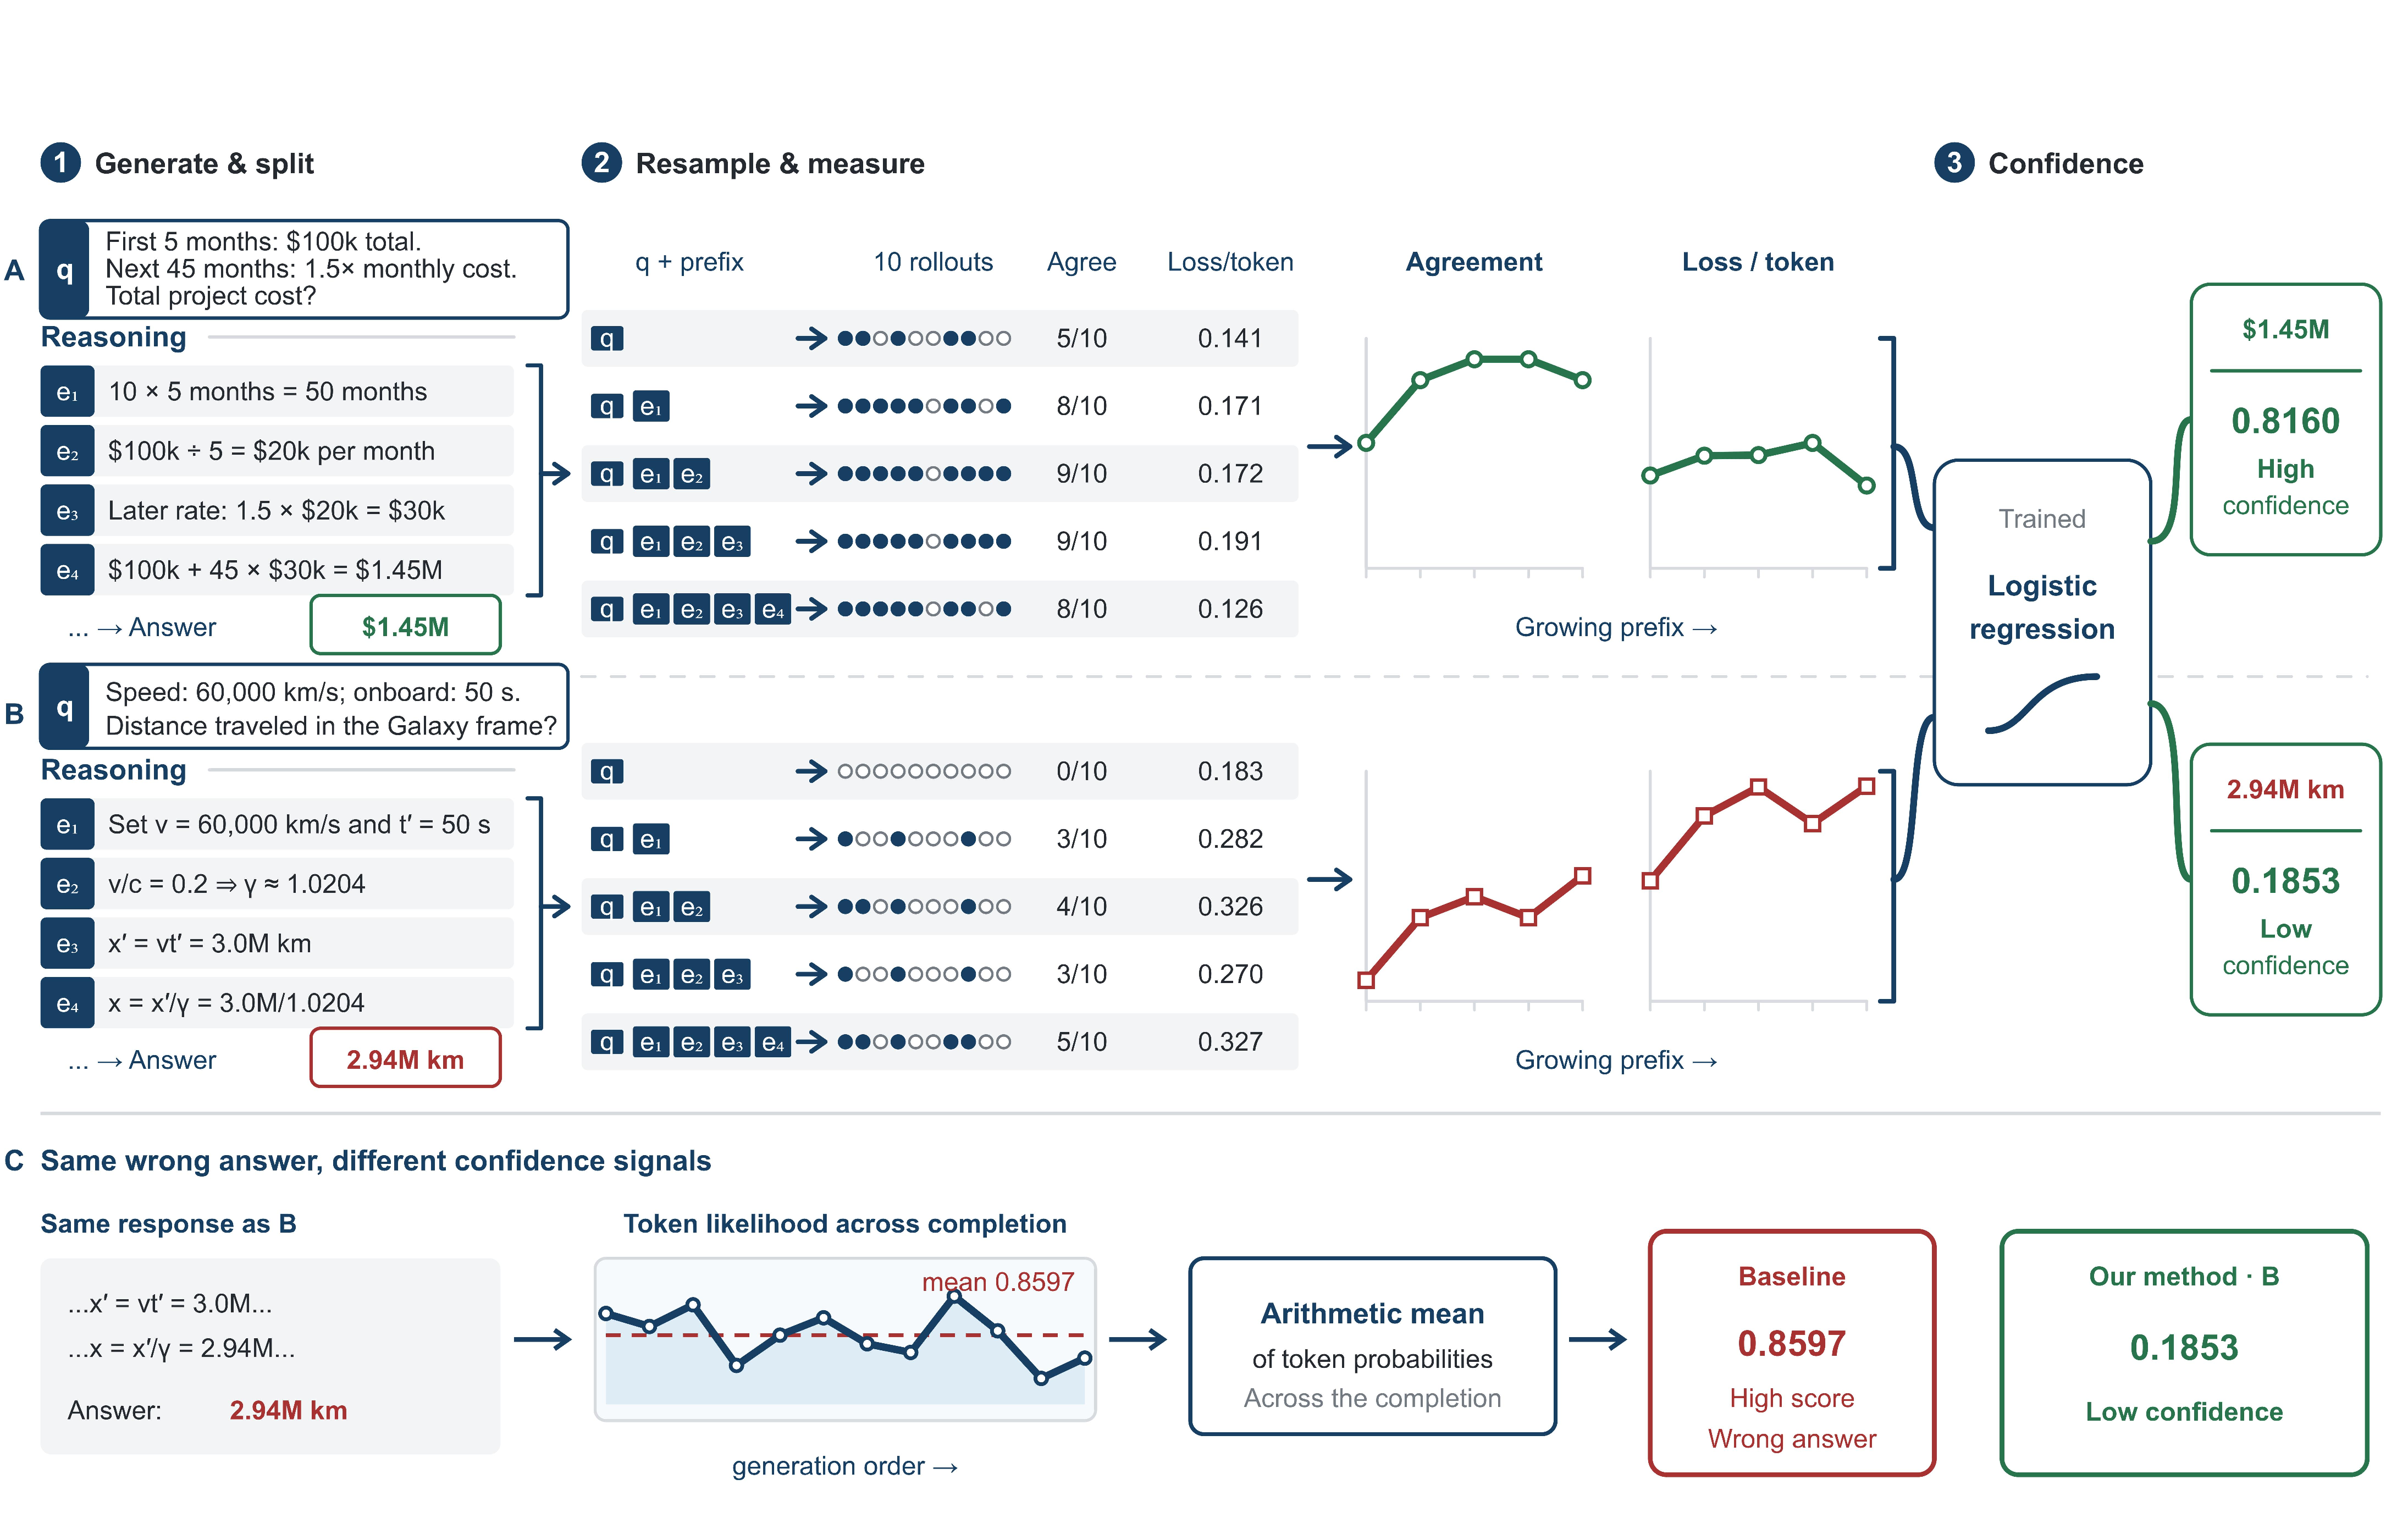
\includegraphics[width=\linewidth]{figures/main_figure.pdf}
    \caption{
    \textbf{Evidence-Guided Confidence Estimation from Reasoning Dynamics.}
    The reasoning chain is divided into sequential evidence segments, from which
    trajectory-level features are extracted using information gain under two
    complementary measures based on \textbf{loss} and \textbf{self-consistency},
    followed by a logistic regression model for confidence estimation.
    \textbf{(A)} A GSM8K example in which the model produces the correct answer;
    the proposed method assigns high confidence, reflecting the progressively
    increasing agreement and informative evidence along the reasoning trajectory.
    \textbf{(B)} A GPQA example in which the model produces an incorrect answer;
    in contrast, the evidence dynamics yield substantially lower confidence,
    despite the model generating a coherent reasoning chain.
    \textbf{(C)} The same incorrect GPQA example as in (B), evaluated using a
    conventional token-probability-based baseline. While the arithmetic mean
    of token probabilities assigns a high confidence score ($0.8597$) to the
    incorrect answer, our method assigns a substantially lower confidence
    score ($0.1853$), highlighting the difference between token-level fluency
    and evidence-based confidence.
    }
    \label{fig:reasoning_confidence}
\end{figure}

Inspired by the \emph{Diffusion Decision Model (DDM)}, a neuroscience model of decision-making in which the drift rate characterizes the strength and direction of evidence accumulation, we view an LLM's reasoning trajectory as a sequential accumulation of evidence toward a final answer. Building on this perspective, we propose a novel information-theoretic approach to estimate the \emph{information gain} of individual evidence items from changes in predictive loss and self-consistency-based agreement probabilities. These evidence-level estimates form a trajectory-level feature representation that captures how informative each reasoning step is for the final answer, enabling \emph{Trajectory-Level Confidence} estimation. We then use a lightweight logistic regression model to predict the probability that the final answer is correct. As illustrated in Figure~\ref{fig:reasoning_confidence}, our approach can assign substantially lower confidence to the incorrect answer in Example B than probability-based confidence measures, which assign a high score despite the incorrect final answer.

We evaluate the proposed approach across eight diverse benchmarks and multiple LLMs. The results demonstrate meaningful improvements in AUROC over existing baselines, while simultaneously reducing the ECE, indicating more accurate and better-calibrated confidence estimates. Our contributions can be summarized as follows:

\begin{itemize}
    \item We propose a \emph{Trajectory-Level Confidence Estimation} framework that derives confidence from the evolution of evidence throughout the reasoning process and can be applied to LLMs in a black-box setting, without requiring access to their internal representations or parameters, while maintaining confidence estimation performance very close to that of the white-box setting.

    \item We introduce an information-theoretic metric for quantifying the \emph{information gain} contributed by individual evidence items in an LLM reasoning trajectory.

    \item We demonstrate consistent improvements in confidence estimation, with modest but meaningful gains in AUROC and reductions in ECE across eight diverse benchmarks and multiple LLMs.
\end{itemize}

\section{Related Work}

\paragraph{Foundations of Confidence Estimation.}
Reliable confidence estimation is crucial for assessing the trustworthiness of LLM outputs, particularly when plausible responses may be incorrect. A common class of approaches derives confidence from the model's predictive distribution, using signals such as token probabilities, entropy, and sequence-level likelihood or cumulative log-probability~\cite{ulmer2024calibrating}. \emph{Self-consistency} uses agreement across multiple reasoning paths as a confidence signal \citep{wang2023self}, while \emph{semantic entropy} measures uncertainty over semantically distinct answers rather than surface forms \citep{kuhn2023semantic}.

\paragraph{Confidence Estimation for LLM Reasoning.}
Recent work has increasingly studied confidence estimation to improve the reliability and efficiency of LLM reasoning. CER~\cite{razghandi-etal-2025-cer} incorporates confidence into self-consistency by weighting sampled reasoning paths according to their estimated reliability. \emph{Learning When to Sample}~\cite{xiong-etal-2026-learning} uses features extracted from reasoning trajectories to estimate confidence and adaptively allocate additional sampling to uncertain instances. \emph{Diagnosing Multi-step Reasoning Failures}~\cite{liu-etal-2026-stepwise} estimates confidence at individual reasoning steps using an Information Bottleneck formulation, enabling the localization of potentially erroneous reasoning. \emph{Beyond the Last Answer}~\cite{hammoud2025beyond} instead evaluates intermediate subthoughts through sampled continuations, aggregating intermediate predictions to improve answer reliability. 

\paragraph{Reasoning-Based Signals for Confidence Estimation}
Recent work increasingly leverages reasoning trajectories and model-internal signals for confidence estimation. Reasoning-trace length has been identified as a simple uncertainty indicator~\cite{devic2025trace}, while internal representations can encode information about reasoning correctness~\cite{chen2026deep}. Other approaches exploit token-level confidence signals to filter unreliable reasoning trajectories~\cite{fu2026deepconf} or improve the reliability of verbalized confidence through extended reasoning~\cite{podolak2025read}. Similarly, token-level predictive distributions have been used to derive self-certainty for best-of-$N$ selection~\cite{kang2025selfcertainty}. Collectively, these studies demonstrate that reasoning trajectories provide informative signals for assessing answer reliability, motivating methods that explicitly quantify how evidence accumulates throughout the reasoning process.


\paragraph{Trajectory-Level Confidence Estimation}
Recent work has moved beyond a single confidence score by modeling how uncertainty evolves throughout the reasoning process. \emph{Tracing Uncertainty in Language Model ``Reasoning''}~\cite{grunefeld2026tracing} estimates token-level uncertainty with respect to both the next token and the final answer across the reasoning trace, and summarizes the resulting uncertainty trajectory using statistical features that can be used by lightweight predictors such as logistic regression. Similarly, \emph{Temporalizing Confidence}~\cite{mao-etal-2025-temporalizing} represents stepwise confidence as a temporal signal and uses Signal Temporal Logic (STL) to characterize patterns such as smoothness, monotonicity, and causal consistency in the confidence trajectory. \emph{Confidence over Time}~\cite{mao-etal-2026-confidence} further mines discriminative STL formulas from stepwise confidence signals to distinguish correct and incorrect reasoning, and uses hypernetworks to adapt their numerical parameters to individual questions. These studies highlight that collapsing the reasoning process into a single final confidence value can discard informative temporal structure, motivating approaches that explicitly model confidence dynamics throughout CoT reasoning.

\begin{figure*}[t]
    \centering
    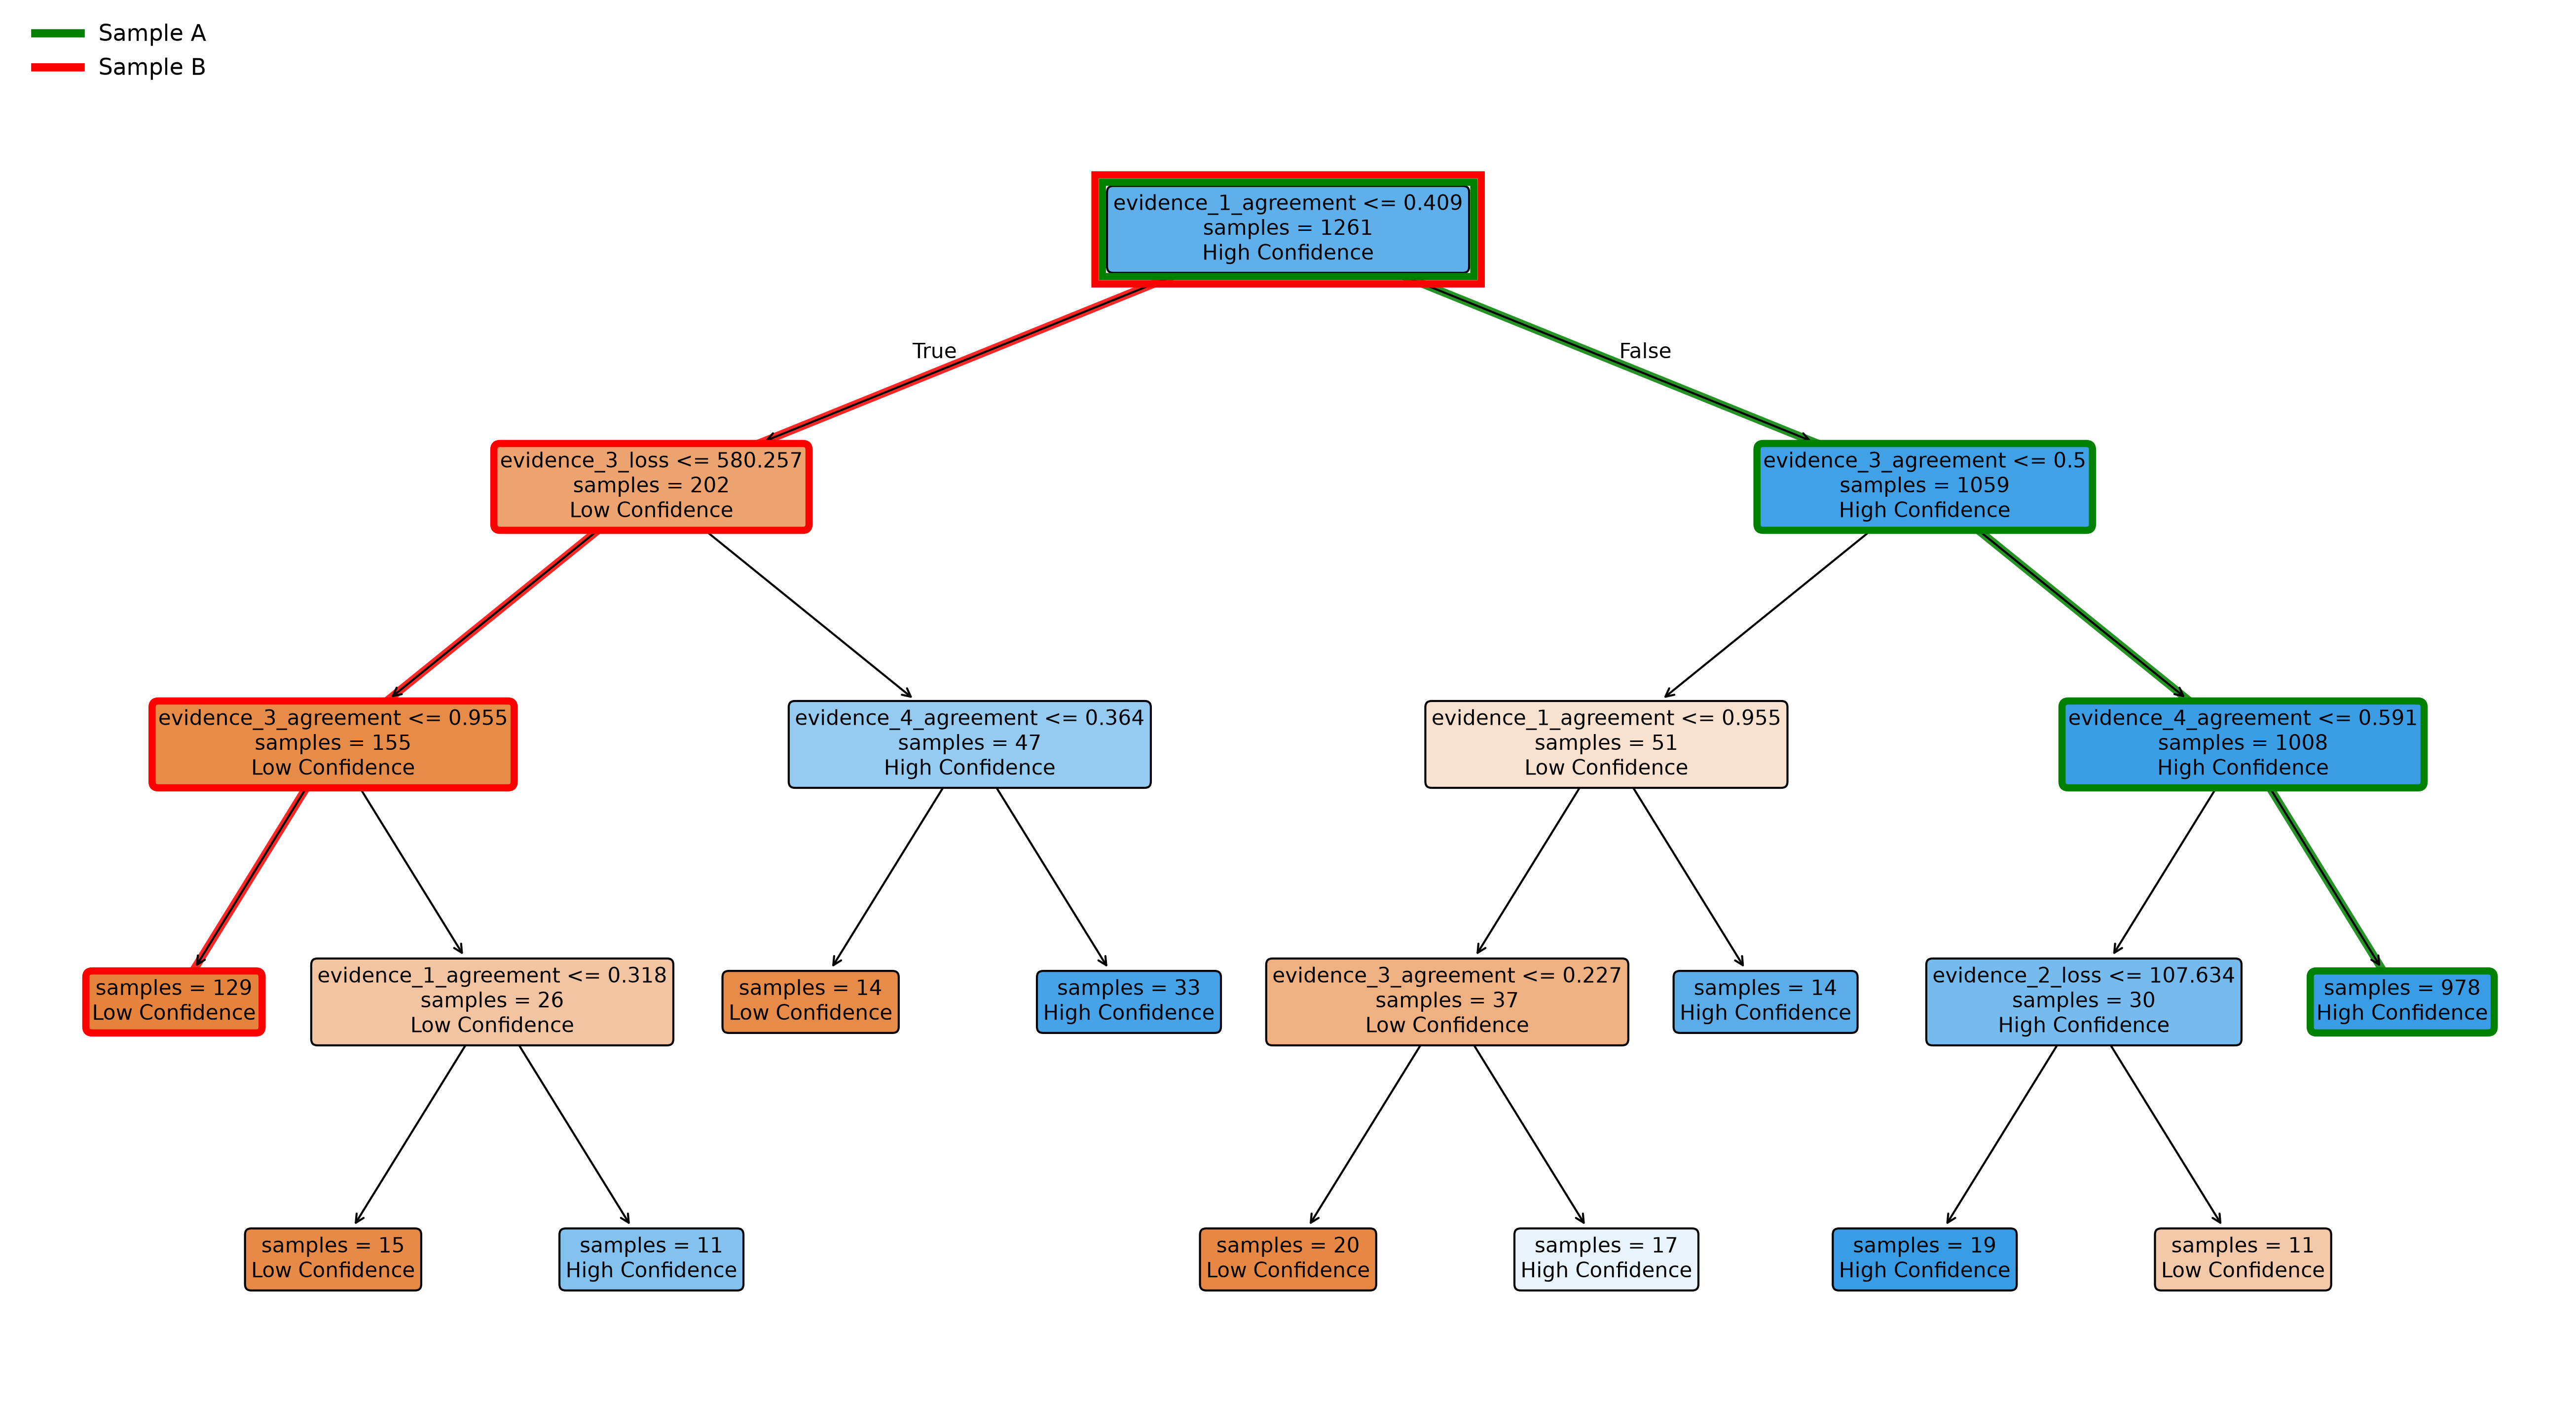
\includegraphics[width=\textwidth]{figures/decision_tree_nv_5_depth_4_leaf_10.png}
    \caption{Decision tree visualization for analyzing feature contributions to confidence estimation. The tree is trained using the features of \textbf{CoT-EIG-Mean} with $K=5$ evidences and is visualized up to depth four. The two highlighted examples illustrate how the learned feature-based decision rules distinguish between high- and low-confidence predictions: (a) a GSM8K example correctly classified as high confidence and (b) a GPQA example classified as low confidence.}
    \label{fig:feature_importance_tree}
\end{figure*}


\section{Method}

\subsection{Diffusion Decision Model}
\label{subsec:diffusion decision model}
The Diffusion Decision Model (DDM)~\citep{ratcliff1978theory,ratcliff2008diffusion} models decision making as sequential evidence accumulation under noise, where a decision is reached when accumulated evidence crosses a decision boundary. A key parameter, the \emph{drift rate} ($v$), captures the rate and direction of evidence accumulation and reflects the quality and discriminativeness of the available information~\citep{ratcliff2002estimating,ratcliff2016diffusion}. Thus, stronger evidence leads to faster accumulation toward the corresponding decision, whereas weak or ambiguous evidence produces slower and less consistent accumulation.

In addition to drift rate, the DDM includes the \emph{boundary separation} ($a$), which represents the amount of evidence required before committing to a decision, and the \emph{starting point} ($z$), which captures an initial bias toward one of the alternatives \citep{ratcliff2002estimating,ratcliff2008diffusion}. The model can therefore distinguish the quality of decision evidence from response caution and decision bias \citep{ratcliff2008diffusion,ratcliff2016diffusion}. 

Overall, the DDM provides a principled framework for interpreting a decision not merely as an outcome, but as the result of an underlying evidence-accumulation process \citep{ratcliff2016diffusion}. This perspective is particularly relevant when intermediate evidence contributing to a decision is available, as it provides a principled basis for relating the quality of such evidence to the strength of the resulting decision process.

\subsection{Quantifying Evidence Quality via Information Gain}
\label{subsec:Quantifying Evidence Quality via Information Gain}

In this work, we develop a DDM-inspired metric to quantify how strongly a chain-of-thought (CoT) reasoning trace influences a LLM's final decision. In the DDM framework, decision-making is viewed as an evidence-accumulation process, where \emph{drift rate} measures the quality of information driving the decision process. Analogously, a LLM first generates a reasoning trace and then produces a final answer based on the accumulated information. We therefore treat the intermediate reasoning states as evidence contributing to the final decision and quantify their influence by measuring how the accumulated reasoning information affects the final answer.

Given a prompt $q$, the LLM generates a reasoning trace $R$ followed by a final answer $Y$, i.e., $q \xrightarrow{\mathrm{LLM}} R \Vert Y$, where $\Vert$ denotes concatenation. We partition the reasoning trace into $k$ sequential evidence segments, $R=e_1\oplus\cdots\oplus e_k$, where $\oplus$ denotes concatenation of evidence segments, and define $C_i$ as the reasoning prefix after observing the first $i$ evidence segments: $C_i=C_{i-1}\oplus e_i$, with $C_0=\emptyset$. Thus, $C_{i-1}$ represents the reasoning state immediately before observing evidence $e_i$, while $C_i$ represents the updated state after incorporating it. The quality of each evidence $e_i$, which we refer to as its \emph{drift rate}, is quantified by its conditional mutual information with the final answer, as defined in Eq.~\ref{eq:evidence_quality}.


\begin{equation}
\mathcal{Q}(e_i)
\equiv
I\left(Y; C_i \mid C_{i-1}\right),
\label{eq:evidence_quality}
\end{equation}

where $I(Y;C_i\mid C_{i-1})$ measures the additional information that $C_i$ provides about the final answer $Y$ beyond $C_{i-1}$. Thus, $\mathcal{Q}(e_i)$ quantifies the incremental, decision-relevant contribution of evidence $e_i$, with larger values indicating greater additional information and smaller values indicating limited contribution beyond the preceding reasoning context. To compute $\mathcal{Q}(e_i)$, we use Equation~\ref{eq:drift_rate_requation_1}; the detailed steps leading from the preceding formulation to this equation are provided in the Appendix~\ref{subsec:proof_evidence_quality}.

\begin{equation}
\mathbb{E}\!\left[\log p\!\left(Y\mid C_i\right)\right]
-
\mathbb{E}\!\left[\log p\!\left(Y\mid C_{i-1}\right)\right]
=
I\!\left(Y;C_i\mid C_{i-1}\right)
.
\label{eq:drift_rate_requation_1}
\end{equation}

Computing $I(Y;C_i\mid C_{i-1})$ requires expensive marginalization over the LLM distribution. To make the measure tractable, we replace the final answer $Y$ with $Y_{>i}$, the continuation of the reasoning chain from $e_i$ through the final answer. This preserves the underlying interpretation while enabling efficient estimation of the information contributed by each evidence segment. Accordingly, Equation~(\ref{eq:drift_rate_requation_1}) is replaced by Equation~(\ref{eq:drift_rate_requation_2}).


\begin{equation}
\mathbb{E}\!\left[\log p\!\left(Y_{>i}\mid C_i\right)\right]
-
\mathbb{E}\!\left[\log p\!\left(Y_{>i}\mid C_{i-1}\right)\right]
=
I\!\left(Y_{>i};C_i\mid C_{i-1}\right)
.
\label{eq:drift_rate_requation_2}
\end{equation}

The quantity $\mathbb{E}[\log p(Y_{>i}\mid C_i)]$ is estimated using Eq.~\ref{eq:monte_carlo_estimator}, with $Y$ fixed to the final answer generated in the initial trajectory. Here, $\mathcal{L}(C_i,Y_{>i})$ denotes the sequence-level loss of the complete sequence $C_i\Vert Y_{>i}$, while $\log p(C_i)=-\mathcal{L}(C_i)$ denotes the log-probability of the reasoning prefix. Rollout trajectories that do not produce the same final answer $Y$ are excluded from the estimation. The detailed derivation is provided in Appendix~\ref{subsec:proof_drift_rate_requation_2}.

\begin{equation}
\widehat{
\mathbb{E}
\left[
\log p(Y_{>i}\mid C_i)
\right]
}
=
-\frac{1}{N_{\mathrm{succ}}}
\sum_{n=1}^{N}
\mathbf{1}\!\left[Y^{(n)}=Y\right]
\mathcal{L}
\left(C_i,Y_{>i}^{(n)}\right)
+
\mathcal{L}(C_i),
\label{eq:monte_carlo_estimator}
\end{equation}
where
\begin{equation}
N_{\mathrm{succ}}
=
\sum_{n=1}^{N}
\mathbf{1}\!\left[Y^{(n)}=Y\right].
\end{equation}
\subsection{Confidence Estimation via Evidence Information Gain}
\label{subsec:Confidence Estimation Method}

CoT reasoning can improve LLM accuracy~\cite{wei2022chain} and provide signals for confidence estimation. Since evidence-level information gain captures each evidence segment's contribution toward the final answer, its sequence provides a measure of reasoning informativeness. We therefore use these information gains as a \textbf{novel signal} for estimating confidence in the final answer.

Information-gain trajectories may exhibit patterns associated with reasoning uncertainty, such as late surges or substantial fluctuations across evidence segments. In contrast, more consistent trajectories may indicate greater confidence. However, these patterns should not be assumed to transfer directly from human decision-making to LLM reasoning, whose evidence-accumulation dynamics may differ substantially.

In the previous section~\ref{subsec:Quantifying Evidence Quality via Information Gain}, we introduced a method for estimating the information gain of each evidence, where
$\mathbb{E}\!\left[\log p\!\left(Y_{>i}\mid C_i\right)\right]$
is estimated using the LLM's loss on the generated response. Alternatively, we estimate $p\left(Y_{>i}\mid C_i\right)$ via self-consistency by sampling multiple continuations and use the resulting probability as a single estimate of $\mathbb{E}\left[\log p(Y_{>i}\mid C_i)\right]$. While the loss-based approach may provide a more accurate estimate, self-consistency is a \textbf{black-box} method that does not require access to the model's loss or token-level probabilities. In addition to loss- and self-consistency-based estimates, we use their changes between consecutive evidence segments as additional features. For each evidence $i$, we construct the feature tuple defined in Eq.~\ref{eq:feature_tuple}:

\begin{equation}
\mathbf{f}_i =
\left(
e_{\mathrm{loss}}^i,\,
e_{\mathrm{sc}}^i,\,
\Delta_{\mathrm{loss}}^i,\,
\Delta_{\mathrm{sc}}^i
\right),
\qquad
\Delta_{\mathrm{loss}}^i =
e_{\mathrm{loss}}^i - e_{\mathrm{loss}}^{i-1},
\qquad
\Delta_{\mathrm{sc}}^i =
e_{\mathrm{sc}}^i - e_{\mathrm{sc}}^{i-1}.
\label{eq:feature_tuple}
\end{equation}


\begin{equation}
\mathbf{F} =
\left[
\mathbf{f}_1;\mathbf{f}_2;\ldots;\mathbf{f}_k
\right]
\in \mathbb{R}^{4k}.
\label{eq:feature_vector}
\end{equation}

The CoT trace is partitioned into equal-length evidence segments, from which four predefined features are extracted and concatenated into $\mathbf{F}$. Logistic regression then maps $\mathbf{F}$ to the probability of a correct final answer, which serves as the confidence estimate.

\section{Experiments}
\label{sec:experiments}

\subsection{Experimental Setup}
\label{sec:experimental_setup}

\paragraph{Models and Benchmarks.}
We evaluate our confidence estimation method on two open-weight reasoning models, \textsc{DeepSeek-R1-Distill-Qwen-7B}~\cite{guo2025deepseek} and \textsc{Qwen3-8B}~\cite{yang2025qwen3}, across eight benchmarks spanning mathematical, scientific, factual, and general reasoning. The suite includes \textsc{AIME}, \textsc{MATH500}, and \textsc{GSM8K} for mathematical reasoning; \textsc{GPQA}, \textsc{MMLU}, and \textsc{MMLU-Pro} for scientific and academic knowledge; \textsc{TruthfulQA} for factuality; and \textsc{Countdown} for constrained reasoning.


\paragraph{Evaluation Metrics.}
We evaluate confidence quality using \textbf{AUROC}, which measures discrimination between correct and incorrect predictions, and \textbf{Expected Calibration Error (ECE)}, which measures the alignment between predicted confidence and empirical accuracy~\cite{guo2017calibration,kadavath2022language}. Non-probabilistic confidence scores are min--max normalized before computing ECE.


\subsection{Baselines and Proposed Method}

\paragraph{Token-level baselines.}
The token-level baselines compute statistics over the CoT reasoning trace. Specifically, the mean and sum of token-level loss (\textbf{Mean-Loss}, \textbf{Sum-Loss}), entropy (\textbf{Mean-Ent}, \textbf{Sum-Ent}), and token probability (\textbf{Mean-Prob}, \textbf{Sum-Prob}) are considered.

\paragraph{Representation-based baseline.}
\textbf{LastRep} uses the final-layer representation of the CoT as input to a logistic regression classifier trained to predict answer correctness. The classifier's output probability is used as the confidence estimate.

\paragraph{Self-consistency baselines.}
\textbf{SC-10} generates 10 independent rollouts for each question, with confidence estimated from the agreement among their final answers. To provide a computationally matched comparison, \textbf{SC-Budget} increases the self-consistency sampling budget to $25$, $50$, $75$, $100$, and $125$ rollouts for $K \in \{5,10,15,20,25\}$, respectively, where $K$ denotes the number of evidences in the chain-of-thought reasoning trace. These budgets approximately match the computational cost of our method with 10 rollouts per evidence.

\paragraph{Proposed method.}
The proposed method, denoted as \textbf{CoT-EIG}, first generates the complete response with a temperature of 0.2 and divides the CoT into $K$ consecutive evidences. For each evidence, 10 rollout continuations are generated using a temperature of 1.0 to extract information-gain-based features. Two variants based on token aggregation are considered: \textbf{CoT-EIG-Mean}, which averages the features over tokens, and \textbf{CoT-EIG-Sum}, which sums them.

\begin{table}[t]
    \centering
    \caption{Confidence estimation performance of different baselines and the proposed CoT-EIG method on Qwen3-8B and DeepSeek-R1-Distill-Qwen-7B, using 5 CoT evidences. Results are reported as mean $\pm$ standard deviation over 50 independent runs.}
    \label{tab:confidence_results}
    \resizebox{\linewidth}{!}{%
    \begin{tabular}{lcc|cc}
        \toprule
        \multirow{2}{*}{Method} &
        \multicolumn{2}{c|}{Qwen3-8B} &
        \multicolumn{2}{c}{DeepSeek-R1-Distill-Qwen-7B} \\
        & AUROC $\uparrow$ & ECE $\downarrow$
        & AUROC $\uparrow$ & ECE $\downarrow$ \\
        \midrule

        \multicolumn{5}{c}{\textit{Token-level baselines}} \\
        \midrule

        Mean-Ent
        & $0.61 \pm 0.02$
        & $0.22 \pm 0.02$
        & $0.58 \pm 0.02$
        & $0.17 \pm 0.02$ \\

        Sum-Ent
        & $0.62 \pm 0.02$
        & $0.22 \pm 0.01$
        & $0.60 \pm 0.02$
        & $0.24 \pm 0.01$ \\

        Mean-Loss
        & $0.61 \pm 0.02$
        & $0.23 \pm 0.02$
        & $0.57 \pm 0.02$
        & $0.16 \pm 0.02$ \\

        Sum-Loss
        & $0.62 \pm 0.02$
        & $0.22 \pm 0.01$
        & $0.60 \pm 0.02$
        & $0.24 \pm 0.01$ \\

        Mean-Prob
        & $0.58 \pm 0.02$
        & $0.17 \pm 0.01$
        & $0.58 \pm 0.02$
        & $0.23 \pm 0.01$ \\

        \midrule

        \multicolumn{5}{c}{\textit{Representation-based baseline}} \\
        \midrule

        LastRep
        & $0.60 \pm 0.02$
        & $0.28 \pm 0.01$
        & $0.58 \pm 0.02$
        & $0.31 \pm 0.01$ \\

        \midrule

        \multicolumn{5}{c}{\textit{Self-consistency baselines}} \\
        \midrule

        SC-10
        & $0.69 \pm 0.02$
        & $0.18 \pm 0.02$
        & $0.71 \pm 0.02$
        & $0.16 \pm 0.01$ \\

        SC-Budget
        & $0.78 \pm 0.02$
        & $0.15 \pm 0.01$
        & --- & --- \\

        \midrule

        \multicolumn{5}{c}{\textit{Proposed method}} \\
        \midrule

        CoT-EIG-Mean
        & $\mathbf{0.84 \pm 0.01}$
        & $\mathbf{0.11 \pm 0.01}$
        & $0.83 \pm 0.01$
        & $\mathbf{0.08 \pm 0.01}$ \\

        CoT-EIG-Sum
        & $0.81 \pm 0.02$
        & $0.12 \pm 0.01$
        & $\mathbf{0.84 \pm 0.01}$
        & $0.13 \pm 0.01$ \\

        \bottomrule
    \end{tabular}%
    }
\end{table}

\subsection{Cross-Benchmark Generalization}
\label{sec:cross_benchmark_generalization}
We evaluate the generalization of confidence estimation using a domain-based holdout protocol. For each target benchmark, the estimator is trained on the remaining benchmarks and evaluated on the held-out benchmark. For example, MATH500, GSM8K, and AIME form the mathematical reasoning domain, while MMLU and MMLU-Pro form the multiple-choice knowledge domain. Each benchmark is used once as the target, and results are averaged across all holdout evaluations. All experiments are repeated 50 times using bootstrap resampling with replacement under different random seeds. Given the low sampling temperature (0.2), repeated model generations are not used as an additional source of variability; instead, run-to-run variability is estimated through bootstrap resampling. The mean and standard deviation are reported across the 50 runs.

Overall, the CoT-EIG variants consistently achieve higher AUROC and lower 
ECE than the token-level and self-consistency baselines, as shown in 
Figure~\ref{fig:auroc_ece_comparison}. On Qwen3-8B, CoT-EIG-Mean and CoT-EIG-Sum achieve AUROC values of $0.84$ and $0.81$, with ECE values of $0.11$ and $0.12$, respectively. On DeepSeek-R1-Distill-Qwen-7B, they achieve AUROC values of $0.83$ and $0.84$, with ECE values of $0.08$ and $0.13$, respectively. Detailed results for individual holdout evaluations are provided in the Appendix~\ref{sec:appendix_holdout}.

\begin{figure}[t]
    \centering

    % Qwen3-8B
    \begin{subfigure}{0.48\linewidth}
        \centering
        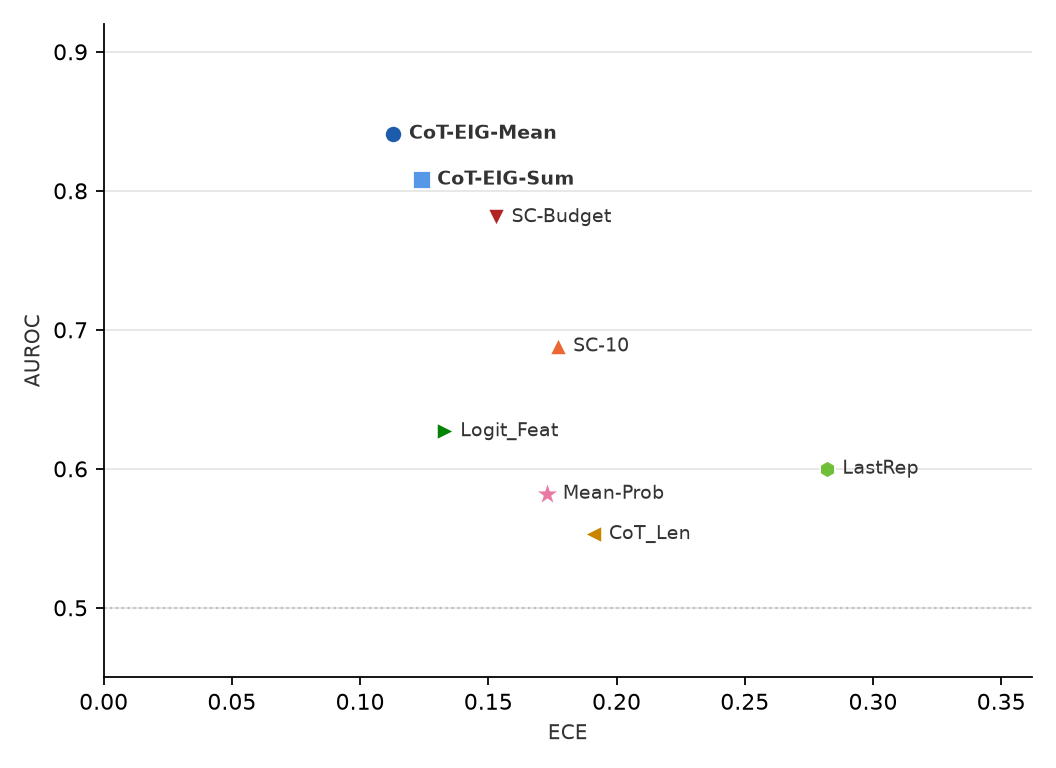
\includegraphics[width=\linewidth]{figures/roc_against_ece_qwen3.png}
        \caption{Qwen3-8B}
        \label{fig:auroc_ece_qwen3}
    \end{subfigure}
    \hfill
    % DeepSeek-R1-Distill-Qwen-7B
    \begin{subfigure}{0.48\linewidth}
        \centering
        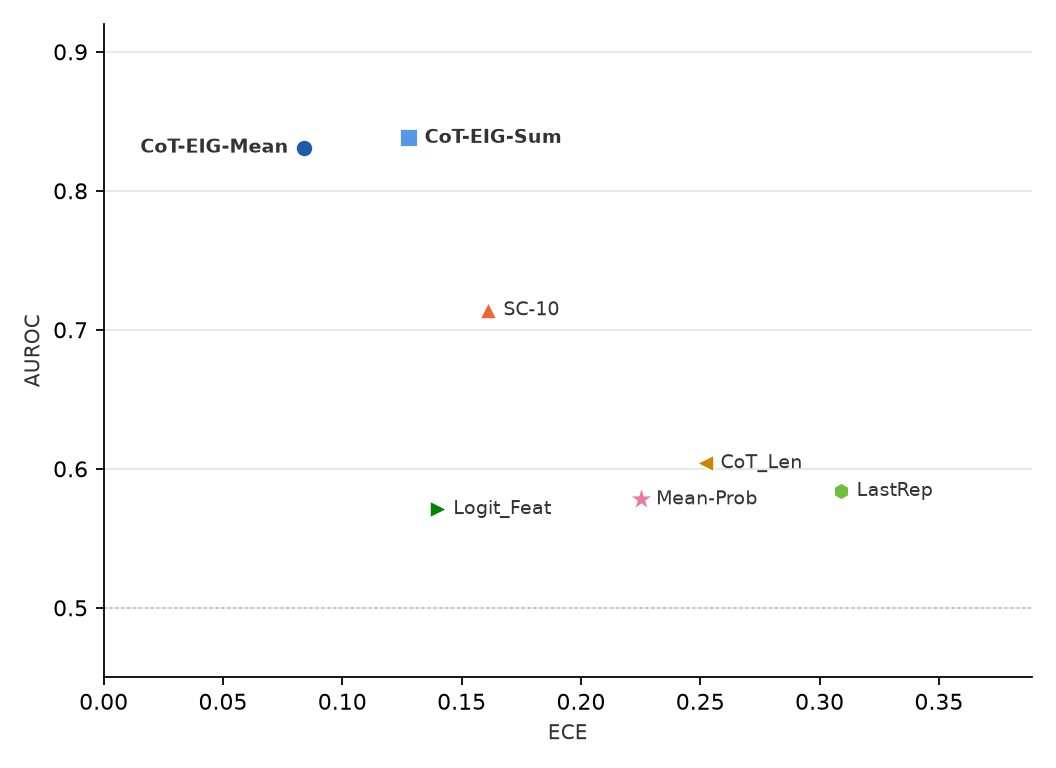
\includegraphics[width=\linewidth]{figures/roc_against_ece_deepseek_r1.png}
        \caption{DeepSeek-R1-Distill-Qwen-7B}
        \label{fig:auroc_ece_deepseek}
    \end{subfigure}

    \caption{Confidence estimation performance of the baselines and proposed
    methods in terms of AUROC and ECE. Each point represents one method,
    with results shown separately for (a) Qwen3-8B and (b)
    DeepSeek-R1-Distill-Qwen-7B. Methods located higher and farther to the
    left correspond to higher AUROC and lower ECE, respectively, and thus
    indicate better confidence estimation performance.}
    \label{fig:auroc_ece_comparison}
\end{figure}


\subsection{Analysis of Feature Contributions}
\label{sec:feature_contribution}

To better understand how the proposed features contribute to confidence estimation, the estimated confidence scores on the test set are divided into two classes: \textit{high confidence} for probabilities $\geq 0.5$ and \textit{low confidence} for probabilities $< 0.5$. A decision tree is then trained on the proposed features to predict these confidence labels, providing an interpretable view of how individual features contribute to the estimated confidence. The tree is visualized up to depth four. For this analysis, \textbf{CoT-EIG-Mean} with $K=5$ evidences is considered.

As shown in Figure~\ref{fig:feature_importance_tree}, features from multiple evidences are used as splitting criteria, indicating that confidence estimation relies on information distributed across the reasoning trace. Notably, as shown in Table~\ref{tab:feature_importance}, self-consistency-based features have the highest aggregate feature importance across the internal split nodes, compared with loss-based features, indicating that they contribute more strongly to distinguishing between high- and low-confidence predictions. The non-zero importance of loss-based features indicates that they also contribute to confidence estimation.

\begin{figure*}[t]
    \centering

    \begin{minipage}{0.48\textwidth}
        \centering
        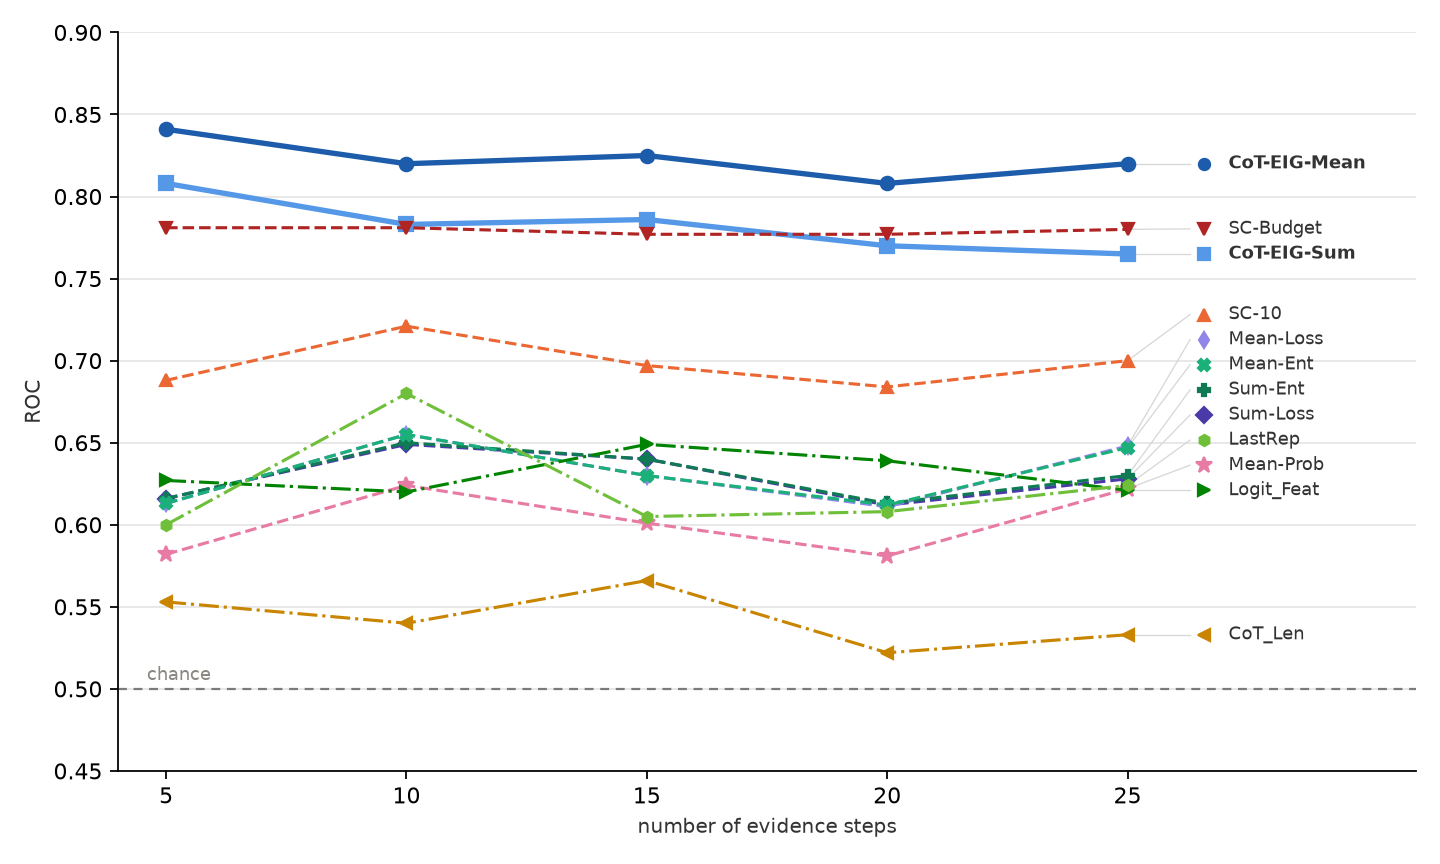
\includegraphics[width=\linewidth]{figures/roc_by_evidence_count_qwen3.png}
        \centerline{(a)}
    \end{minipage}
    \hfill
    \begin{minipage}{0.48\textwidth}
        \centering
        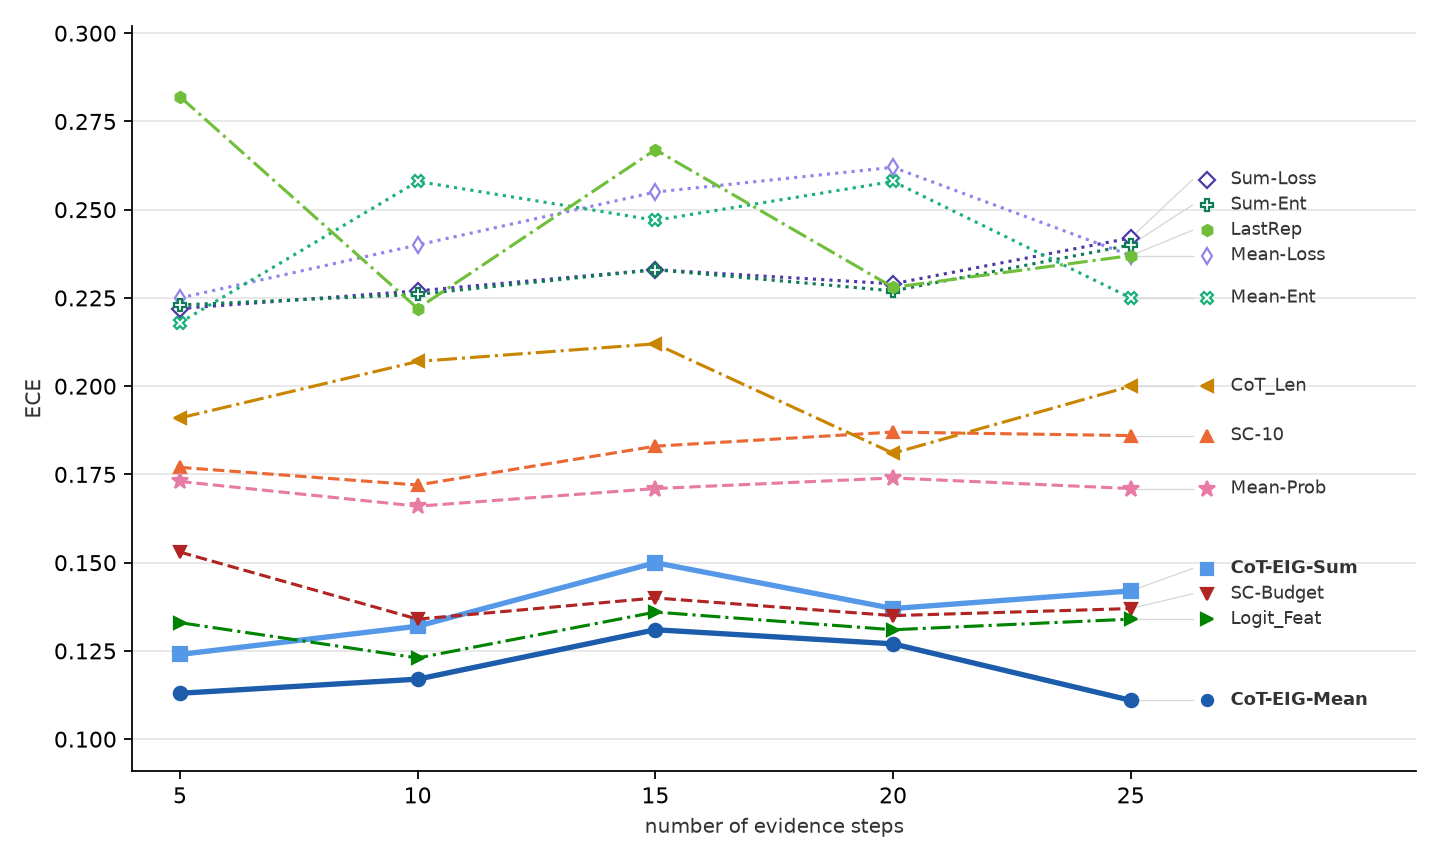
\includegraphics[width=\linewidth]{figures/ece_by_evidence_count_qwen3.png}
        \centerline{(b)}
    \end{minipage}

    \vspace{0.5em}

    \begin{minipage}{0.48\textwidth}
        \centering
        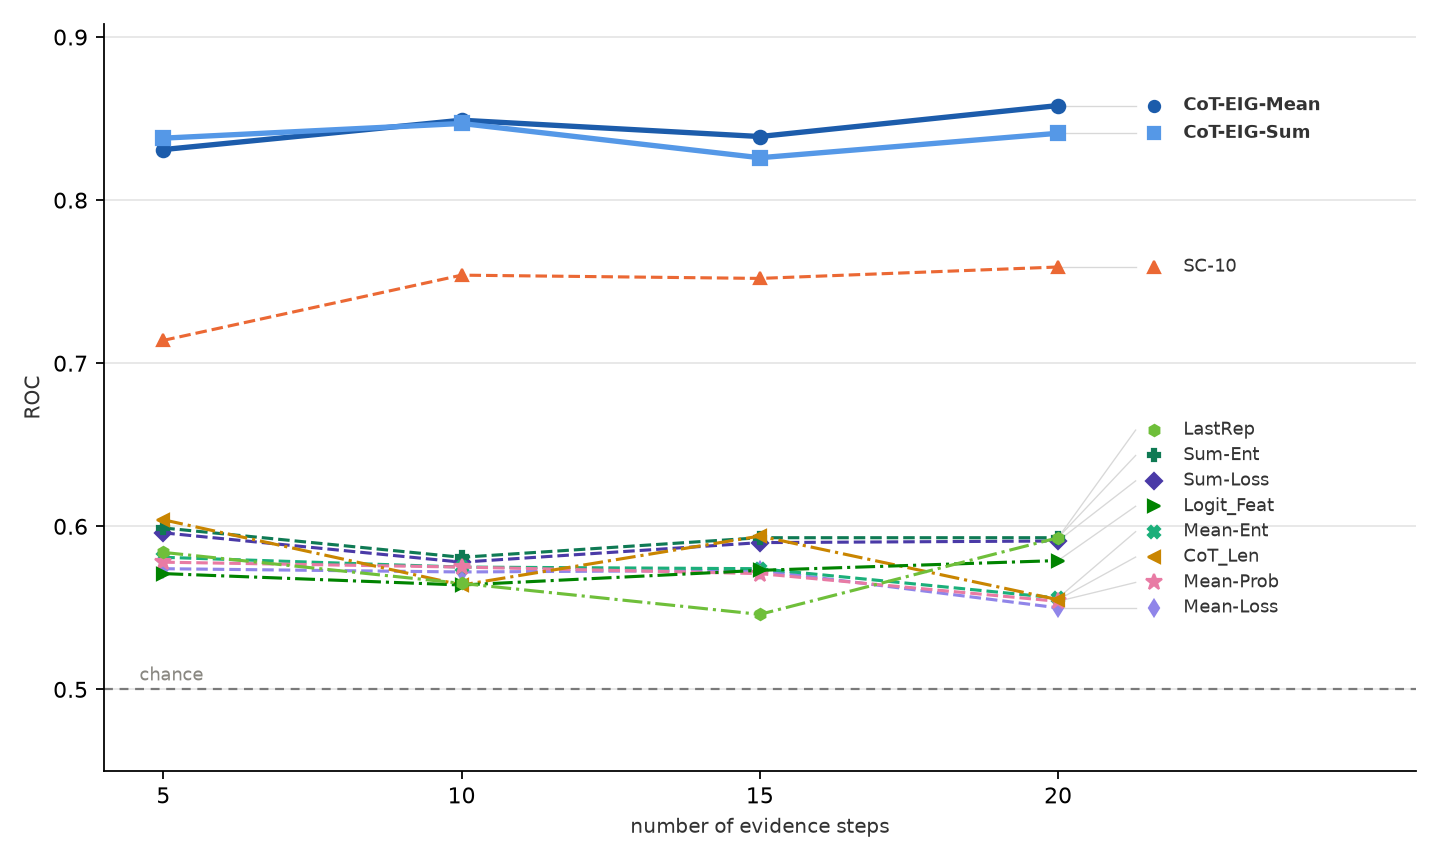
\includegraphics[width=\linewidth]{figures/roc_by_evidence_count_deepseek_r1.png}
        \centerline{(c)}
    \end{minipage}
    \hfill
    \begin{minipage}{0.48\textwidth}
        \centering
        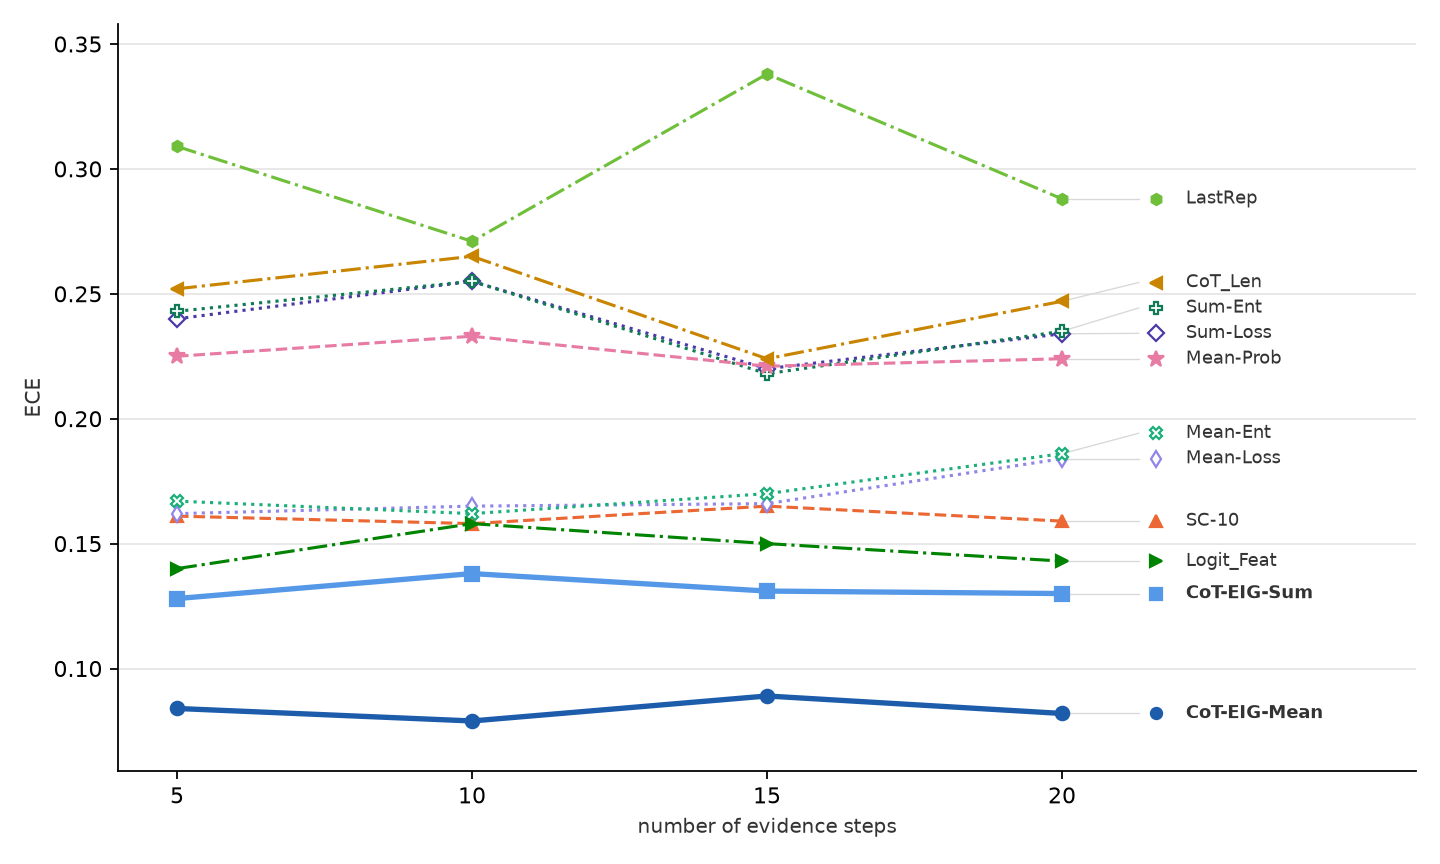
\includegraphics[width=\linewidth]{figures/ece_by_evidence_count_deepseek_r1.png}
        \centerline{(d)}
    \end{minipage}

    \caption{Performance of different confidence estimation baselines across varying numbers of evidences. 
    The top row reports results for Qwen3-8B, while the bottom row reports results for DeepSeek-R1-Distill-Qwen-7B. 
    The left and right columns show AUROC and ECE, respectively.}
    \label{fig:evidence_ablation_models}
\end{figure*}

\section{Ablation Study}

\subsection{Effect of the Number of CoT Evidences}

We first investigate how the number of CoT evidences affects the performance of our confidence estimation method. Specifically, we divide each reasoning trace into 5, 10, 15, 20, or 25 evidences and recompute all features used by our confidence estimator for each setting. This analysis allows us to assess whether the proposed approach is sensitive to the granularity at which the reasoning process is decomposed. By varying the number of evidences while keeping the remaining components of the method unchanged, we characterize the effect of evidence granularity on confidence estimation performance.

Figure~\ref{fig:evidence_ablation_models} shows the effect of varying the number of CoT evidences on confidence estimation performance. Although both AUROC and ECE exhibit minor fluctuations across different numbers of evidences, the overall results remain relatively stable. This suggests that increasing or decreasing the number of evidences does not substantially affect the confidence estimation performance across the evaluated settings. Since the evaluation covers a diverse set of benchmarks, detailed results for each individual benchmark are provided in Appendix~\ref{sec:appendix_holdout}.

\subsection{Effect of Computational Budget}

We next examine whether the performance gains persist under a comparable computational budget. To this end, our method is compared with the computationally matched self-consistency baseline, \textbf{SC-Budget}, whose rollout budget is adjusted according to the number of evidences, denoted by $K$, to approximately match the computational cost of our method. Since self-consistency generally benefits from additional samples, this comparison evaluates whether the gains of our approach persist when the baseline is given a substantially larger sampling budget.

Figure~\ref{fig:evidence_ablation_models} shows that, on Qwen3-8B, \textbf{SC-Budget} performs worse than \textbf{CoT-EIG-Mean} and achieves performance comparable to \textbf{CoT-EIG-Sum}. These results suggest that \textbf{CoT-EIG-Mean} provides a meaningful improvement over self-consistency even under a comparable computational budget.


\subsection{Ablation Study of Feature Sets}
\label{sec:ablation_features}

An ablation study is conducted to examine the contribution of different feature sets to confidence estimation.Six feature sets are considered: \textbf{CoT-EIG}, which uses all four proposed features; \textbf{EIG-SC}, which uses only the self-consistency-based features; \textbf{EIG-Loss}, which uses only the loss-based features; \textbf{Logit\_Feat}, which consists of conventional token-level features, including entropy, loss, and probability statistics; \textbf{LastRep}, which uses the final-layer representation of the reasoning trace; and \textbf{CoT\_Len}, which uses the length of the generated response as the feature. All feature sets are used to train the same logistic regression confidence estimator, allowing the effect of the underlying feature representation to be isolated.

\begin{figure}[t]
    \centering

    % Qwen3-8B
    \begin{subfigure}{\linewidth}
        \centering
        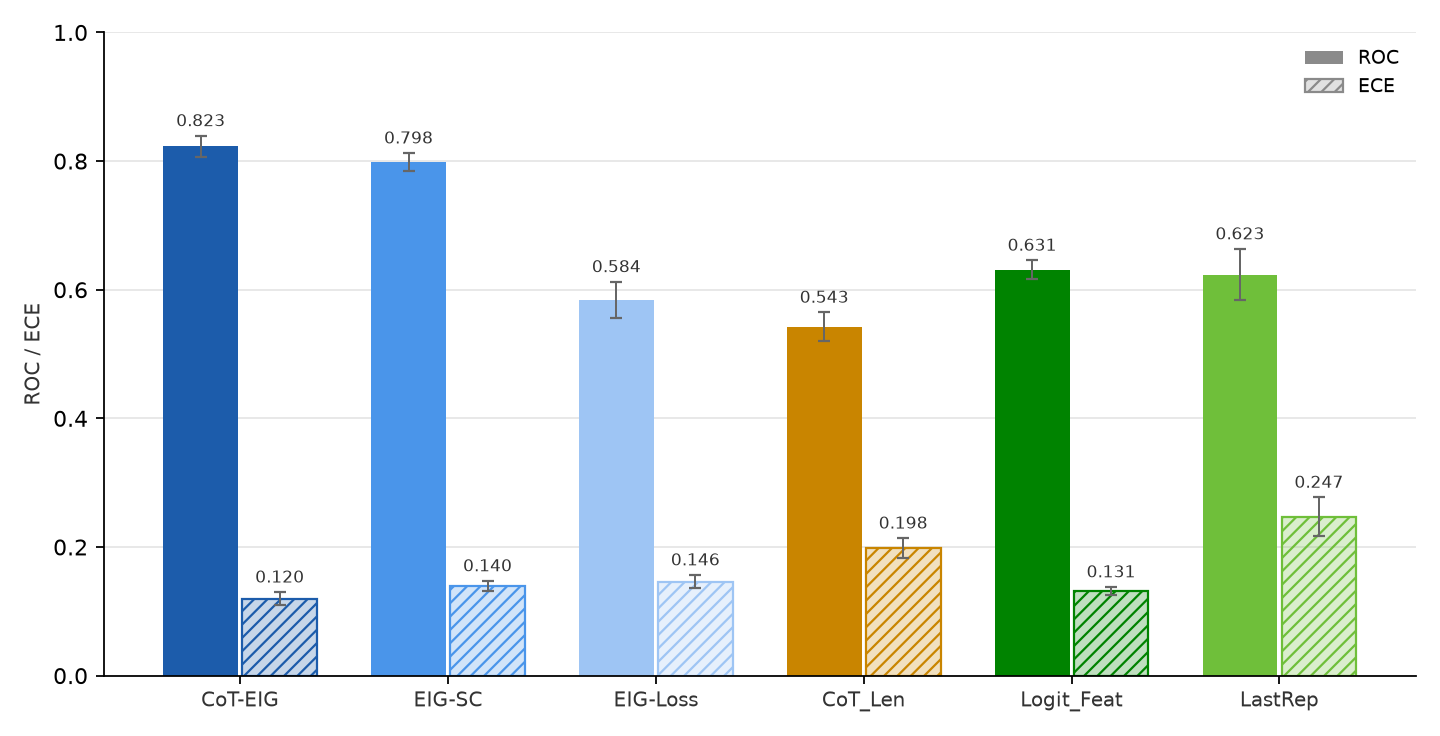
\includegraphics[width=\linewidth]{figures/roc_ece_by_feature_set_qwen3.png}
        \caption{Qwen3-8B}
        \label{fig:feature_ablation_qwen3}
    \end{subfigure}

    \vspace{0.5em}

    % DeepSeek-R1-Distill-Qwen-7B
    \begin{subfigure}{\linewidth}
        \centering
        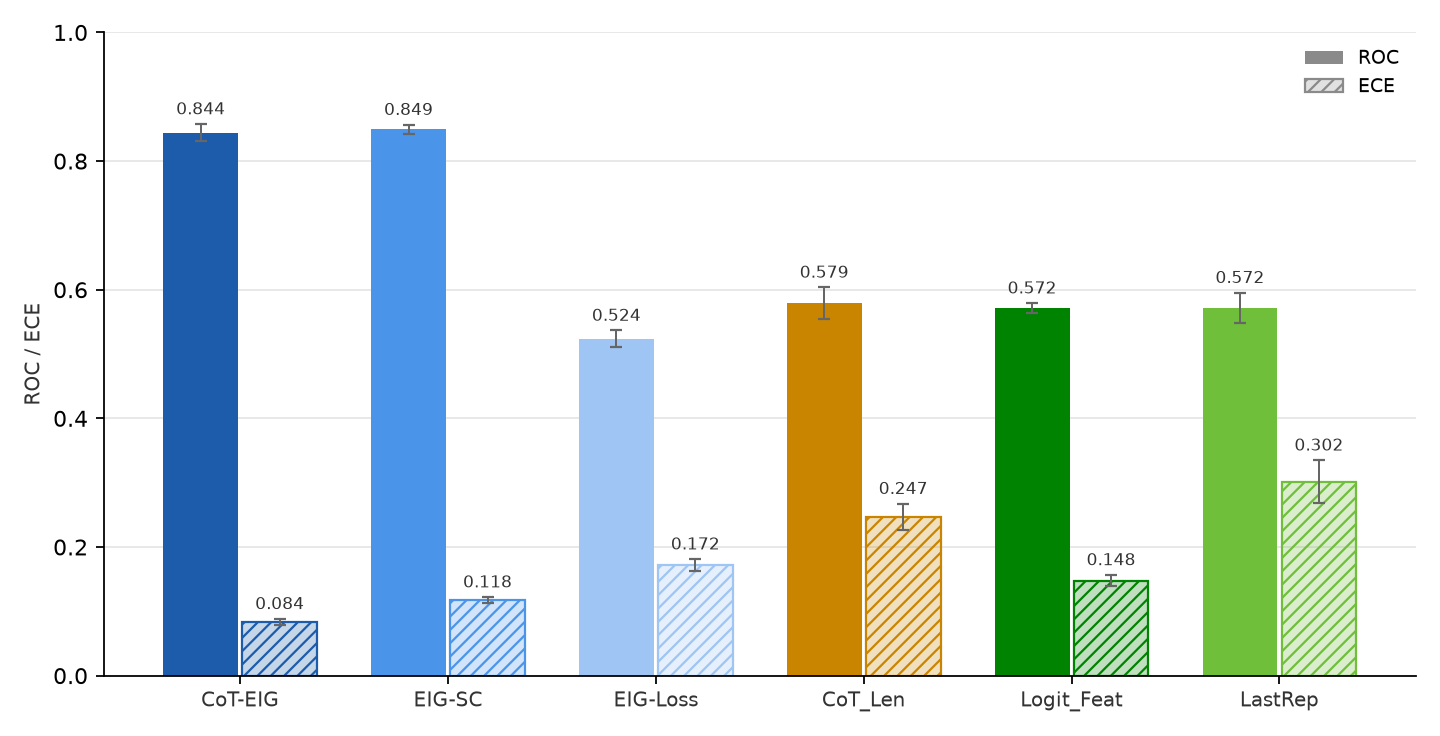
\includegraphics[width=\linewidth]{figures/roc_ece_by_feature_set_deepseek_r1.png}
        \caption{DeepSeek-R1-Distill-Qwen-7B}
        \label{fig:feature_ablation_deepseek}
    \end{subfigure}

    \caption{Ablation study of different feature sets for confidence estimation on two language models. 
    The top and bottom panels report results for Qwen3-8B and DeepSeek-R1-Distill-Qwen-7B, respectively.}
    \label{fig:feature_ablation}
\end{figure}

Although \textbf{CoT-EIG} already combines both loss- and self-consistency (SC)-based features, it achieves the strongest overall performance, with improvements in AUROC and reductions in ECE, the EIG-SC variant performs very close to this full feature set, as shown in Figure~\ref{fig:feature_ablation}. In contrast, EIG-Loss does not exhibit a comparable performance. Within the CoT-EIG framework, incorporating loss features provides a modest improvement in ECE while either improving or maintaining AUROC across the evaluated settings. These results suggest that SC-based features can provide performance close to the full CoT-EIG feature set when the underlying LLM is accessible only as a black box.

\subsection{Conclusion}
In this work, we estimate LLM confidence by modeling Chain-of-Thought as sequential evidence toward the final answer. Inspired by the Diffusion Decision Model, we quantify the information gain of reasoning steps and use the resulting evidence-accumulation patterns as confidence features. Across eight benchmarks and two reasoning models, our approach consistently improves AUROC and reduces ECE compared with existing methods, while maintaining comparable performance in both white-box and black-box settings, showing that reasoning trajectories provide effective confidence signals without requiring access to model internals.

More broadly, confidence estimation is an important metacognitive capability of  LLMs and should ideally be assessed independently of their task-solving ability. By modeling confidence continuously throughout the reasoning trajectory, trajectory-level confidence estimation may capture evolving uncertainty that is missed by a single final confidence score. This perspective motivates further research into the temporal dynamics of confidence and its relationship to prediction correctness.

\subsection*{AI use statement}
We used generative AI tools primarily as an alternative to conventional internet search.
Information obtained through these tools was subsequently reviewed and independently
verified against relevant sources to validate its accuracy.

The authors take full responsibility for the final content of this work, including all
text, claims, analyses, and research artifacts, regardless of whether generative AI
tools were used in their preparation.

\subsection*{Ethics Statement}
This work uses publicly available datasets and pretrained language models and
does not involve human subjects, personally identifiable information, or
sensitive data. We are not aware of significant ethical concerns arising from
this work. By estimating confidence in LLM outputs, our approach may help
reduce concerns associated with over-reliance on potentially incorrect or
uncertain outputs by making uncertainty more explicit.

\subsection*{Reproducibility statement}
To support reproducibility, we conducted the experiments with multiple independent
runs and evaluated the proposed method across multiple models and benchmarks.
The main hyperparameters and experimental settings are reported in the paper,
with additional implementation details provided in the supplementary materials.
The complete source code, experimental outputs, and information required to
access the datasets are provided in the accompanying GitHub repository.

\bibliography{iclr2027_conference}
\bibliographystyle{iclr2027_conference}

\appendix
\section{Proofs}

\subsection{}
\label{subsec:proof_evidence_quality}

\[
\begin{aligned}
\mathbb{E}\!\left[\log p\!\left(Y \mid C_i\right)\right]
-
\mathbb{E}\!\left[\log p\!\left(Y \mid C_{i-1}\right)\right]
&=
\mathbb{E}\!\left[
\log
\frac{p\!\left(Y \mid C_i\right)}
     {p\!\left(Y \mid C_{i-1}\right)}
\right] \\[4pt]
&=
\mathbb{E}\!\left[
\log
\frac{p\!\left(Y \mid C_i,C_{i-1}\right)}
     {p\!\left(Y \mid C_{i-1}\right)}
\right] \\[4pt]
&=
\mathbb{E}\!\left[
\log
\frac{
p\!\left(Y,C_i \mid C_{i-1}\right)
}{
p\!\left(Y \mid C_{i-1}\right)
p\!\left(C_i \mid C_{i-1}\right)
}
\right] \\[4pt]
&=
I\!\left(Y;C_i \mid C_{i-1}\right).
\end{aligned}
\]


\subsection{}
\label{subsec:proof_drift_rate_requation_2}

By the chain rule:
\[
\mathbb{E}
\left[
\log p(Y_{>i}\mid C_i)
\right]
=
\mathbb{E}
\left[
\log
\frac{p(C_i,Y_{>i})}{p(C_i)}
\right].
\]

Thus,
\[
\begin{aligned}
\mathbb{E}
\left[
\log p(Y_{>i}\mid C_i)
\right]
&=
\mathbb{E}
\left[
\log p(C_i,Y_{>i})
-
\log p(C_i)
\right] \\
&=
\mathbb{E}
\left[
\log p(C_i,Y_{>i})
\right]
-
\log p(C_i).
\end{aligned}
\]

Using the sequence-level losses
\[
\mathcal{L}(C_i,Y_{>i})
=
-\log p(C_i,Y_{>i}),
\qquad
\mathcal{L}(C_i)
=
-\log p(C_i),
\]
we obtain
\[
\mathbb{E}
\left[
\log p(Y_{>i}\mid C_i)
\right]
=
-
\mathbb{E}
\left[
\mathcal{L}(C_i,Y_{>i})
\right]
+
\mathcal{L}(C_i).
\]

Finally, using $N$ independently sampled continuations
$\{Y_{>i}^{(n)}\}_{n=1}^{N}$, we obtain
\[
\widehat{
\mathbb{E}
\left[
\log p(Y_{>i}\mid C_i)
\right]
}
=
-\frac{1}{N}
\sum_{n=1}^{N}
\mathcal{L}
\left(C_i,Y_{>i}^{(n)}\right)
+
\mathcal{L}(C_i).
\]

\begin{table}[t]
\centering
\caption{Feature importance based on the fitted decision tree, with higher-importance evidence--feature pairs reported in descending order. The decision tree is fitted on the combined data from all benchmarks evaluated using Qwen3-8B.}
\label{tab:feature_importance}
\begin{tabular}{ccc}
\toprule
\textbf{Evidence} & \textbf{Feature} & \textbf{Importance} \\
\midrule
1 & self-consistency        & 0.6393 \\
3 & self-consistency        & 0.1184 \\
3 & loss             & 0.0847 \\
4 & self-consistency        & 0.0539 \\
1 & loss             & 0.0304 \\
2 & delta\_loss      & 0.0219 \\
5 & loss             & 0.0094 \\
2 & delta\_self-consistency & 0.0084 \\
4 & delta\_self-consistency & 0.0083 \\
3 & delta\_loss      & 0.0078 \\
4 & delta\_loss      & 0.0070 \\
2 & loss             & 0.0056 \\
5 & self-consistency        & 0.0028 \\
5 & delta\_self-consistency & 0.0020 \\
\bottomrule
\end{tabular}
\end{table}

\clearpage

\section{Results for Each Held-Out Group}
\label{sec:appendix_holdout}

\subsection{Multiple-Choice Knowledge Domain}
\label{subsec:appendix_holdout_mcq}

\begin{table}[h]
    \centering
    \caption{Same as Table~\ref{tab:confidence_results}, with the multiple-choice knowledge domain (MMLU and MMLU-Pro) held out.}
    \label{tab:holdout_mcq}
    \resizebox{\linewidth}{!}{%
    \begin{tabular}{lcc|cc}
        \toprule
        \multirow{2}{*}{Method} &
        \multicolumn{2}{c|}{Qwen3-8B} &
        \multicolumn{2}{c}{DeepSeek-R1-Distill-Qwen-7B} \\
        & AUROC $\uparrow$ & ECE $\downarrow$
        & AUROC $\uparrow$ & ECE $\downarrow$ \\
        \midrule
        \multicolumn{5}{c}{\textit{Token-level baselines}} \\
        \midrule
        Mean-Ent & $0.66 \pm 0.02$ & $0.20 \pm 0.02$ & $0.54 \pm 0.03$ & $0.14 \pm 0.03$ \\
        Sum-Ent & $0.67 \pm 0.02$ & $0.21 \pm 0.02$ & $0.59 \pm 0.02$ & $0.27 \pm 0.02$ \\
        Mean-Loss & $0.65 \pm 0.02$ & $0.20 \pm 0.04$ & $0.54 \pm 0.03$ & $0.12 \pm 0.04$ \\
        Sum-Loss & $0.66 \pm 0.02$ & $0.21 \pm 0.02$ & $0.58 \pm 0.02$ & $0.28 \pm 0.02$ \\
        Mean-Prob & $0.64 \pm 0.03$ & $0.14 \pm 0.02$ & $0.54 \pm 0.03$ & $0.24 \pm 0.02$ \\
        \midrule
        \multicolumn{5}{c}{\textit{Representation-based baseline}} \\
        \midrule
        LastRep & $0.58 \pm 0.02$ & $0.30 \pm 0.02$ & $0.57 \pm 0.02$ & $0.34 \pm 0.02$ \\
        \midrule
        \multicolumn{5}{c}{\textit{Self-consistency baselines}} \\
        \midrule
        SC-10 & $0.70 \pm 0.02$ & $0.09 \pm 0.02$ & $0.72 \pm 0.02$ & $0.15 \pm 0.02$ \\
        SC-Budget & $0.79 \pm 0.02$ & $0.12 \pm 0.02$ & --- & --- \\
        \midrule
        \multicolumn{5}{c}{\textit{Proposed method}} \\
        \midrule
        CoT-EIG-Mean & $\mathbf{0.84 \pm 0.02}$ & $\mathbf{0.05 \pm 0.01}$ & $0.85 \pm 0.02$ & $\mathbf{0.06 \pm 0.01}$ \\
        CoT-EIG-Sum & $0.81 \pm 0.02$ & $\mathbf{0.05 \pm 0.01}$ & $\mathbf{0.86 \pm 0.01}$ & $0.09 \pm 0.01$ \\
        \bottomrule
    \end{tabular}%
    }
\end{table}


\begin{figure}[h]
    \centering
    \begin{subfigure}{0.48\linewidth}
        \centering
        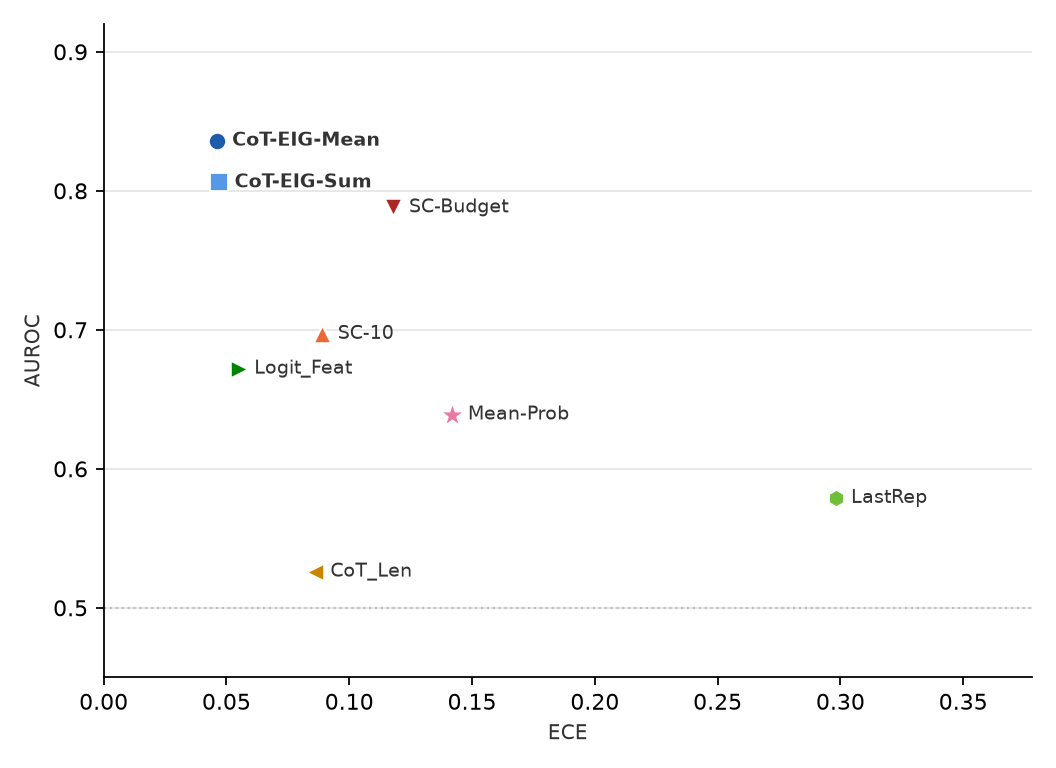
\includegraphics[width=\linewidth]{figures/appendix/roc_against_ece_qwen3_mcq.png}
        \caption{Qwen3-8B}
    \end{subfigure}
    \hfill
    \begin{subfigure}{0.48\linewidth}
        \centering
        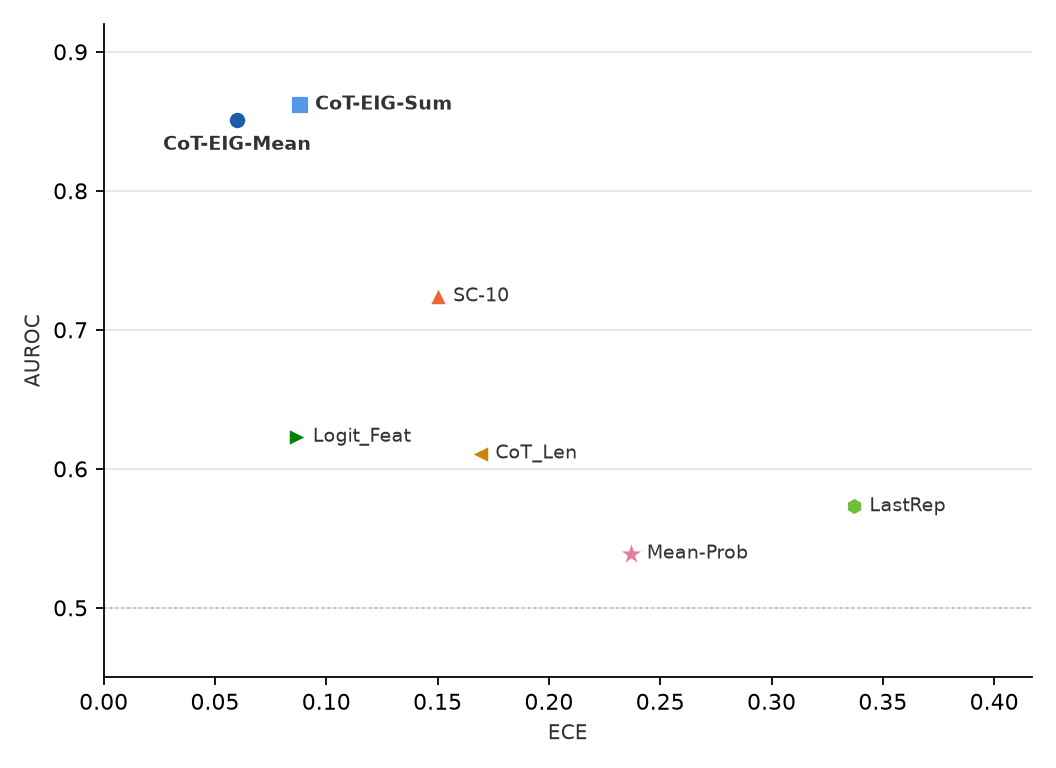
\includegraphics[width=\linewidth]{figures/appendix/roc_against_ece_deepseek_r1_mcq.png}
        \caption{DeepSeek-R1-Distill-Qwen-7B}
    \end{subfigure}
    \caption{Same as Figure~\ref{fig:auroc_ece_comparison}, with the multiple-choice knowledge domain (MMLU and MMLU-Pro) held out.}
    \label{fig:holdout_auroc_ece_mcq}
\end{figure}

\begin{figure}[h]
    \centering
    \begin{minipage}{0.48\textwidth}
        \centering
        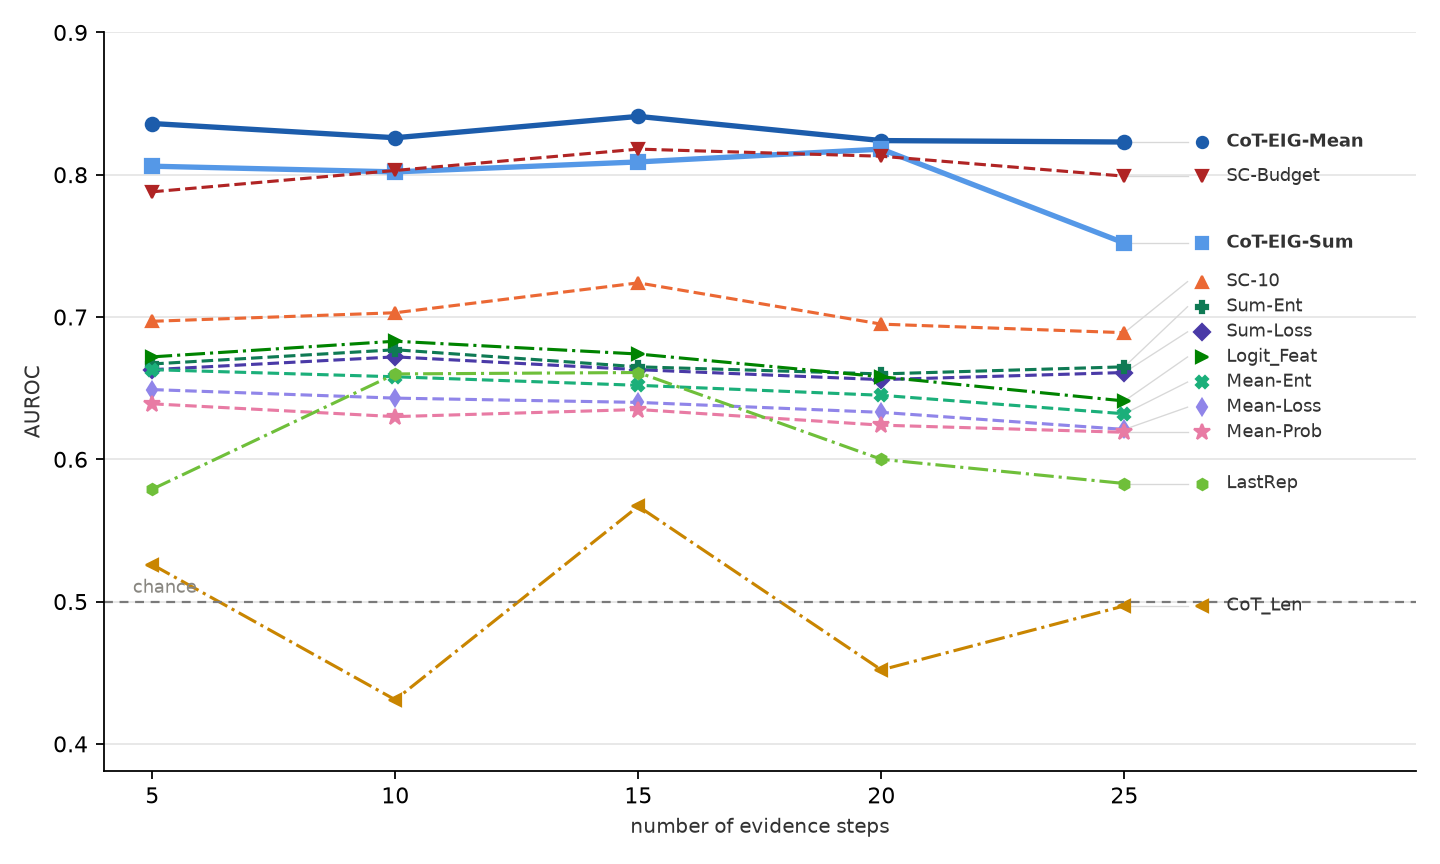
\includegraphics[width=\linewidth]{figures/appendix/roc_by_evidence_count_qwen3_mcq.png}
        \centerline{(a) Qwen3-8B, AUROC}
    \end{minipage}
    \hfill
    \begin{minipage}{0.48\textwidth}
        \centering
        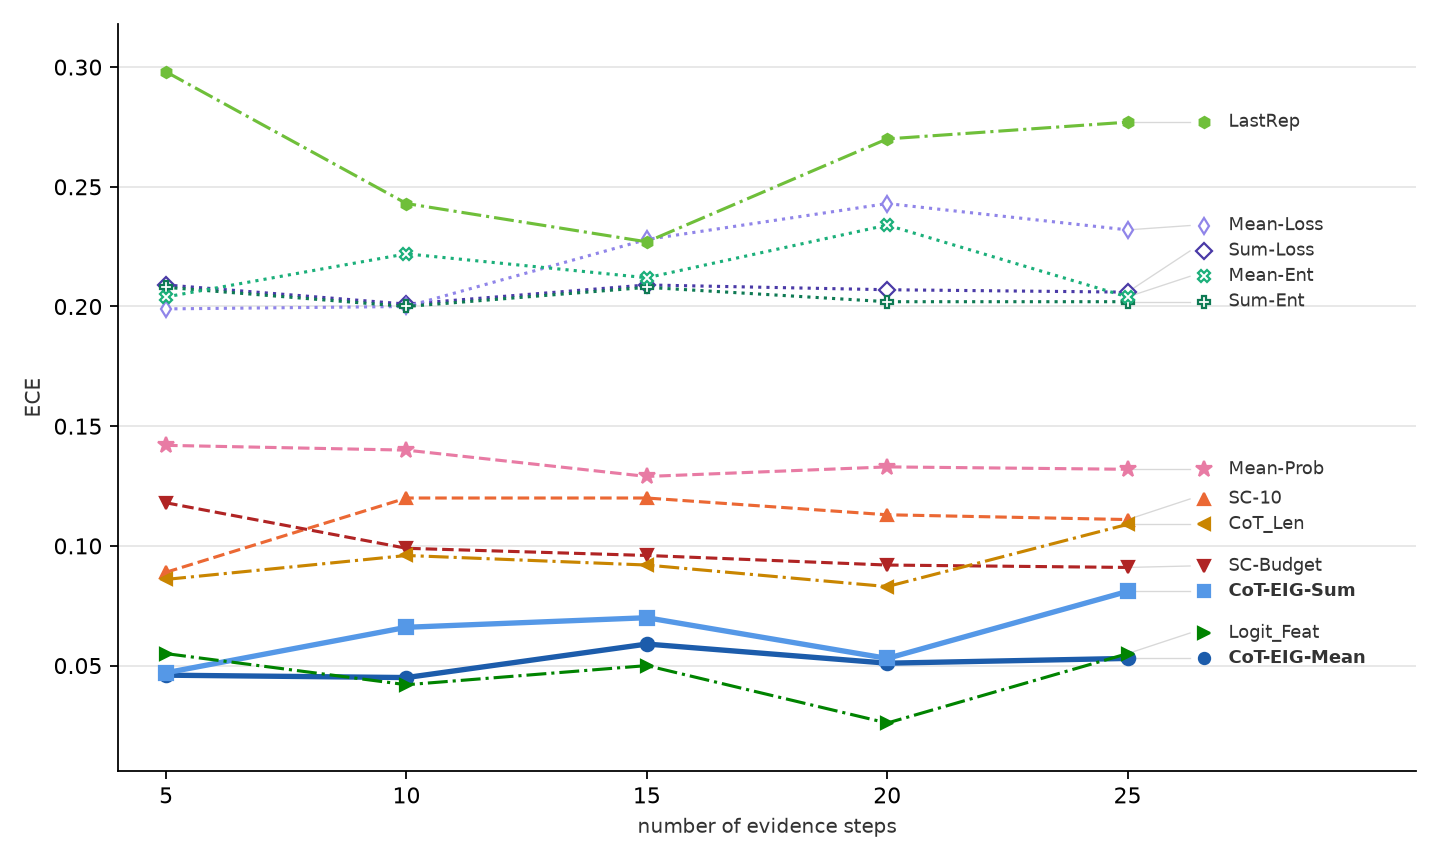
\includegraphics[width=\linewidth]{figures/appendix/ece_by_evidence_count_qwen3_mcq.png}
        \centerline{(b) Qwen3-8B, ECE}
    \end{minipage}

    \vspace{0.5em}

    \begin{minipage}{0.48\textwidth}
        \centering
        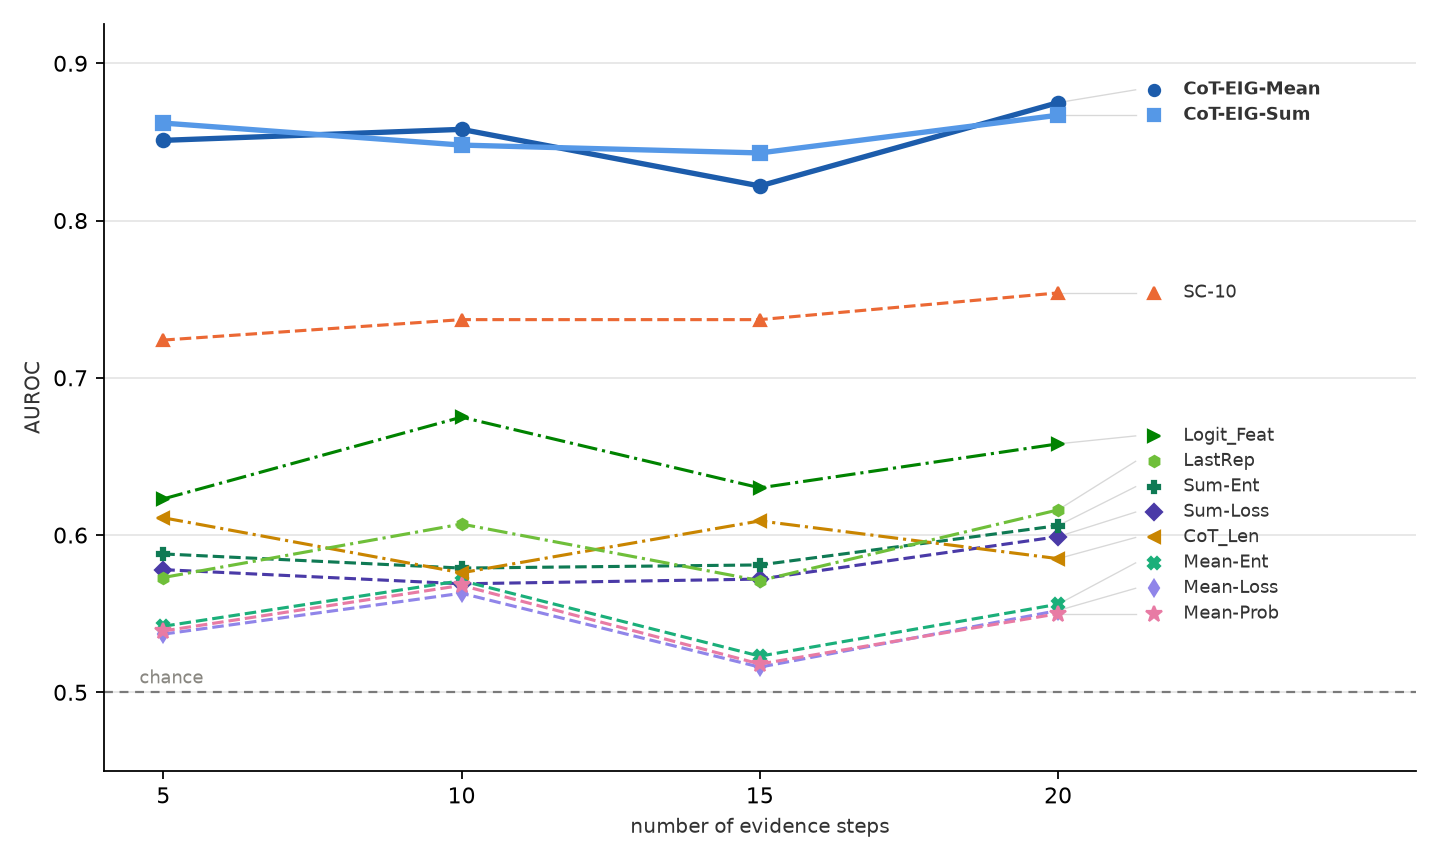
\includegraphics[width=\linewidth]{figures/appendix/roc_by_evidence_count_deepseek_r1_mcq.png}
        \centerline{(c) DeepSeek-R1-Distill-Qwen-7B, AUROC}
    \end{minipage}
    \hfill
    \begin{minipage}{0.48\textwidth}
        \centering
        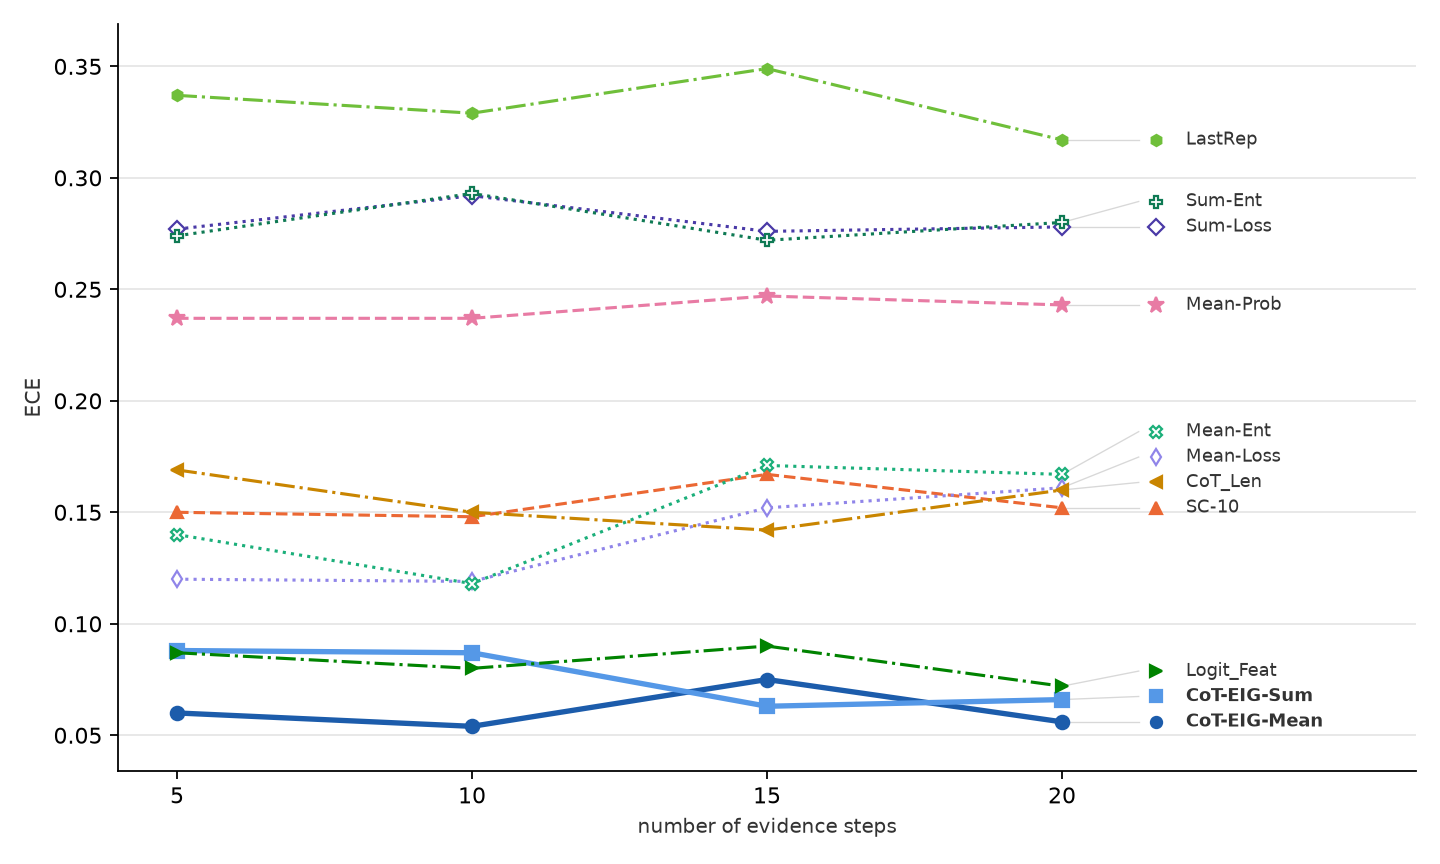
\includegraphics[width=\linewidth]{figures/appendix/ece_by_evidence_count_deepseek_r1_mcq.png}
        \centerline{(d) DeepSeek-R1-Distill-Qwen-7B, ECE}
    \end{minipage}
    \caption{Same as Figure~\ref{fig:evidence_ablation_models}, with the multiple-choice knowledge domain (MMLU and MMLU-Pro) held out.}
    \label{fig:holdout_evidence_mcq}

    \vspace{1.5em}

    % Side by side rather than stacked, so this figure fits on the page above with it.
    \begin{subfigure}{0.48\linewidth}
        \centering
        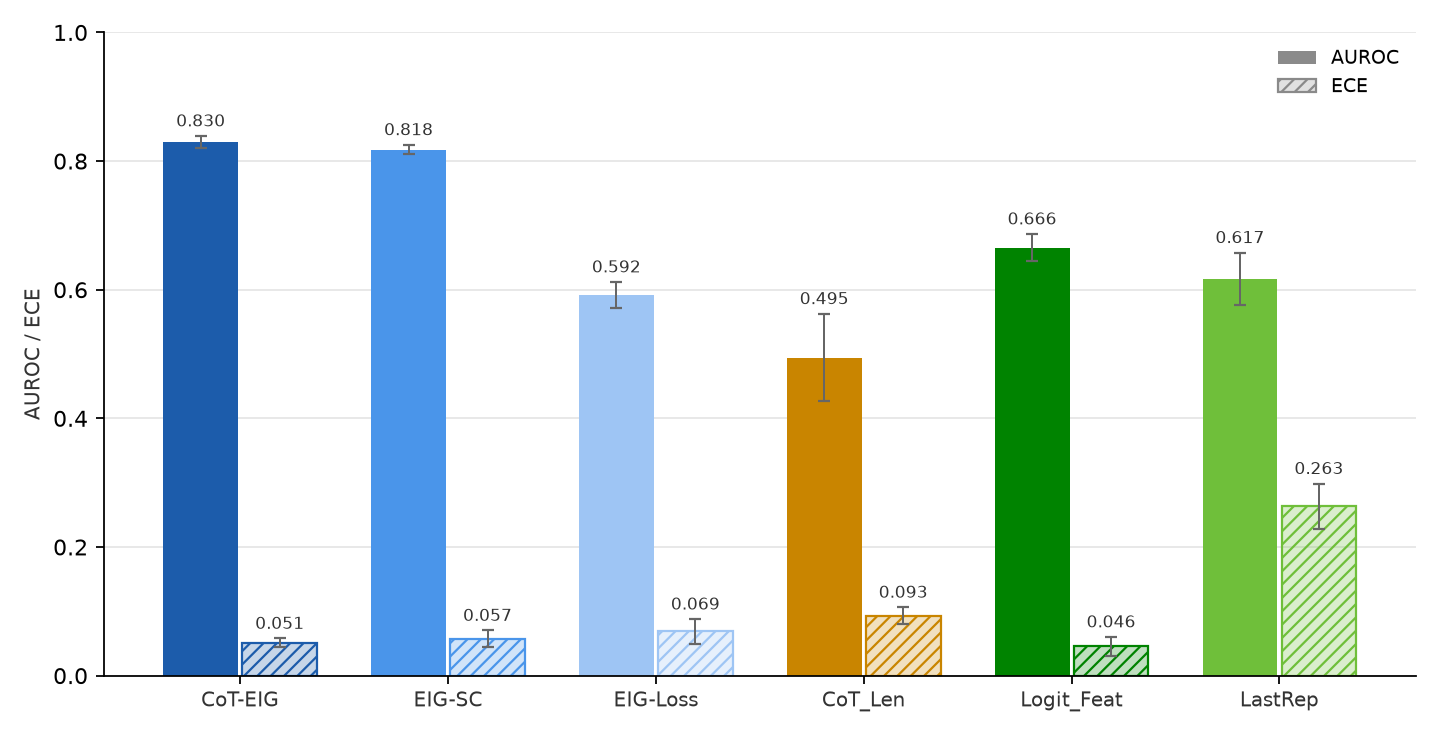
\includegraphics[width=\linewidth]{figures/appendix/roc_ece_by_feature_set_qwen3_mcq.png}
        \caption{Qwen3-8B}
    \end{subfigure}
    \hfill
    \begin{subfigure}{0.48\linewidth}
        \centering
        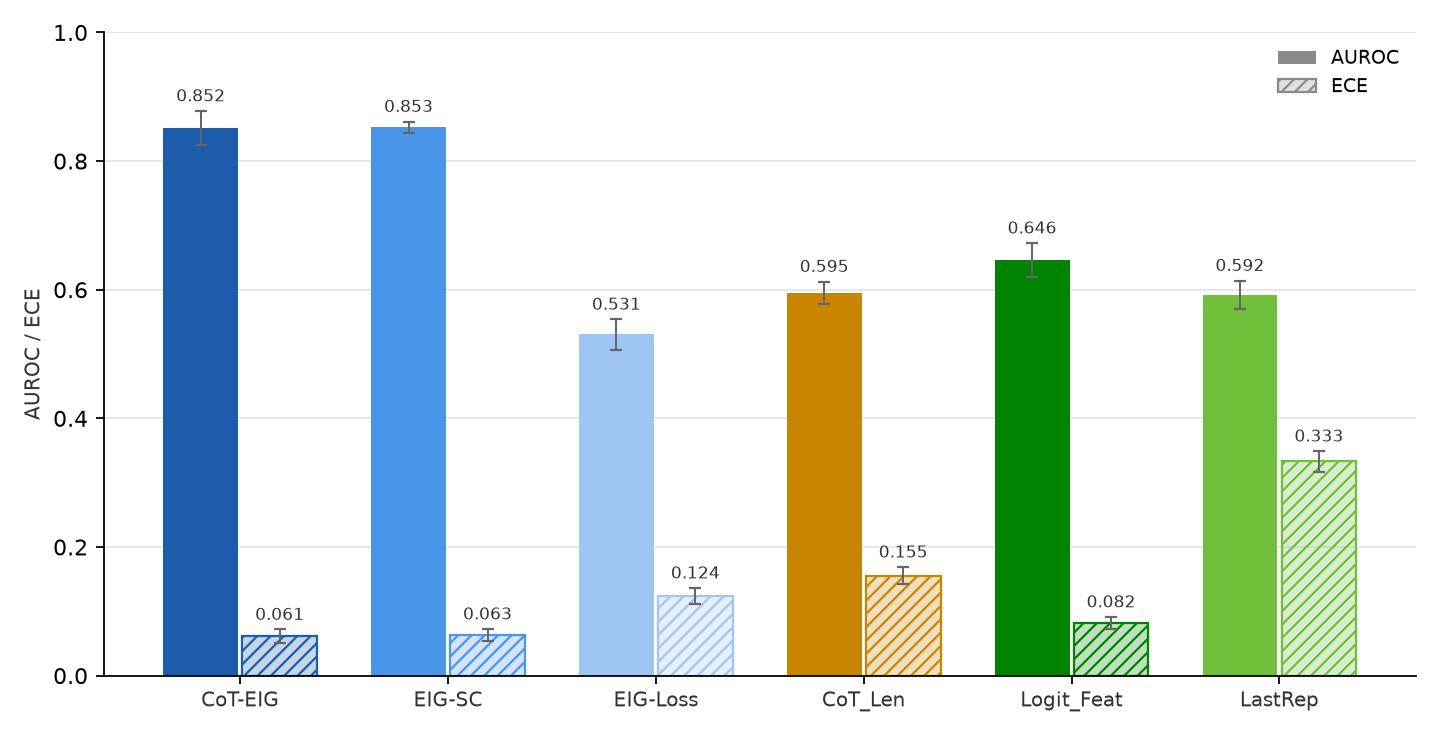
\includegraphics[width=\linewidth]{figures/appendix/roc_ece_by_feature_set_deepseek_r1_mcq.png}
        \caption{DeepSeek-R1-Distill-Qwen-7B}
    \end{subfigure}
    \caption{Same as Figure~\ref{fig:feature_ablation}, with the multiple-choice knowledge domain (MMLU and MMLU-Pro) held out.}
    \label{fig:holdout_feature_ablation_mcq}
\end{figure}

\clearpage

\subsection{Mathematics Domain}
\label{subsec:appendix_holdout_math}

\begin{table}[h]
    \centering
    \caption{Same as Table~\ref{tab:confidence_results}, with the mathematics domain (GSM8K, MATH500 and AIME) held out.}
    \label{tab:holdout_math}
    \resizebox{\linewidth}{!}{%
    \begin{tabular}{lcc|cc}
        \toprule
        \multirow{2}{*}{Method} &
        \multicolumn{2}{c|}{Qwen3-8B} &
        \multicolumn{2}{c}{DeepSeek-R1-Distill-Qwen-7B} \\
        & AUROC $\uparrow$ & ECE $\downarrow$
        & AUROC $\uparrow$ & ECE $\downarrow$ \\
        \midrule
        \multicolumn{5}{c}{\textit{Token-level baselines}} \\
        \midrule
        Mean-Ent & $0.55 \pm 0.06$ & $0.28 \pm 0.06$ & $0.69 \pm 0.05$ & $0.23 \pm 0.02$ \\
        Sum-Ent & $0.61 \pm 0.04$ & $0.10 \pm 0.02$ & $0.66 \pm 0.05$ & $0.06 \pm 0.01$ \\
        Mean-Loss & $0.55 \pm 0.06$ & $0.28 \pm 0.06$ & $0.68 \pm 0.05$ & $0.24 \pm 0.02$ \\
        Sum-Loss & $0.61 \pm 0.05$ & $0.10 \pm 0.02$ & $0.66 \pm 0.05$ & $0.06 \pm 0.01$ \\
        Mean-Prob & $0.48 \pm 0.06$ & $\mathbf{0.05 \pm 0.01}$ & $0.68 \pm 0.05$ & $\mathbf{0.04 \pm 0.01}$ \\
        \midrule
        \multicolumn{5}{c}{\textit{Representation-based baseline}} \\
        \midrule
        LastRep & $0.81 \pm 0.04$ & $\mathbf{0.05 \pm 0.01}$ & $0.64 \pm 0.04$ & $0.20 \pm 0.02$ \\
        \midrule
        \multicolumn{5}{c}{\textit{Self-consistency baselines}} \\
        \midrule
        SC-10 & $0.73 \pm 0.04$ & $0.20 \pm 0.04$ & $0.81 \pm 0.04$ & $0.06 \pm 0.02$ \\
        SC-Budget & $0.86 \pm 0.03$ & $0.07 \pm 0.02$ & --- & --- \\
        \midrule
        \multicolumn{5}{c}{\textit{Proposed method}} \\
        \midrule
        CoT-EIG-Mean & $\mathbf{0.94 \pm 0.03}$ & $0.09 \pm 0.01$ & $0.93 \pm 0.03$ & $\mathbf{0.04 \pm 0.01}$ \\
        CoT-EIG-Sum & $0.92 \pm 0.03$ & $0.14 \pm 0.01$ & $\mathbf{0.94 \pm 0.02}$ & $0.10 \pm 0.01$ \\
        \bottomrule
    \end{tabular}%
    }
\end{table}


\begin{figure}[h]
    \centering
    \begin{subfigure}{0.48\linewidth}
        \centering
        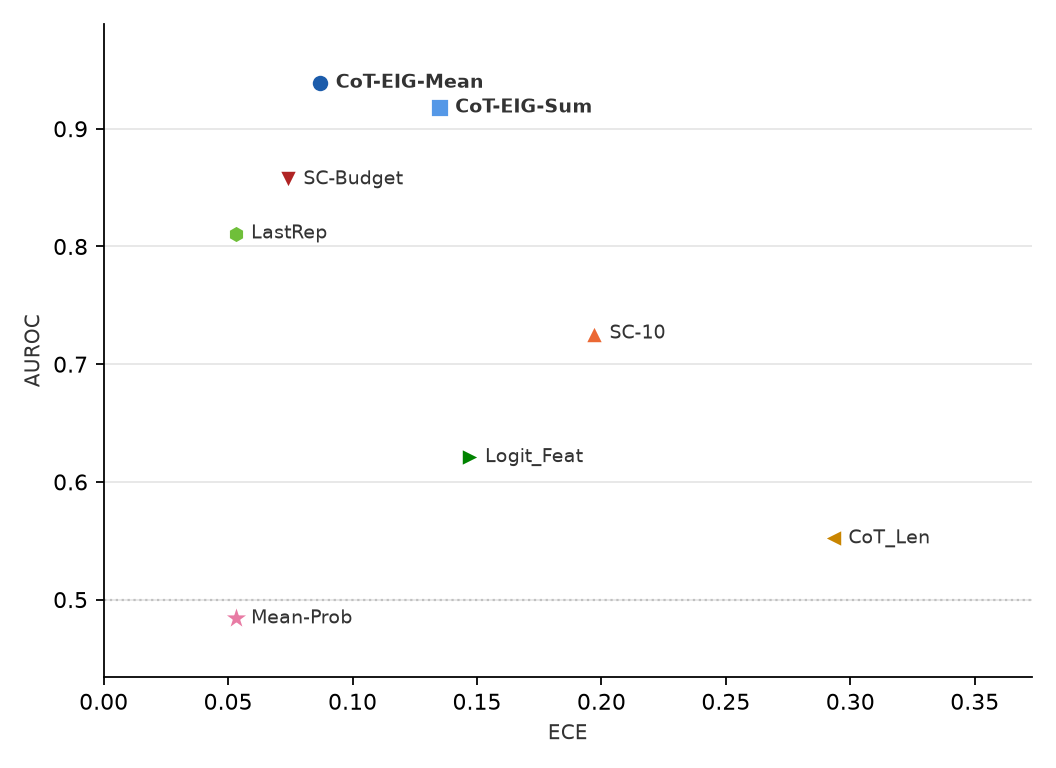
\includegraphics[width=\linewidth]{figures/appendix/roc_against_ece_qwen3_math.png}
        \caption{Qwen3-8B}
    \end{subfigure}
    \hfill
    \begin{subfigure}{0.48\linewidth}
        \centering
        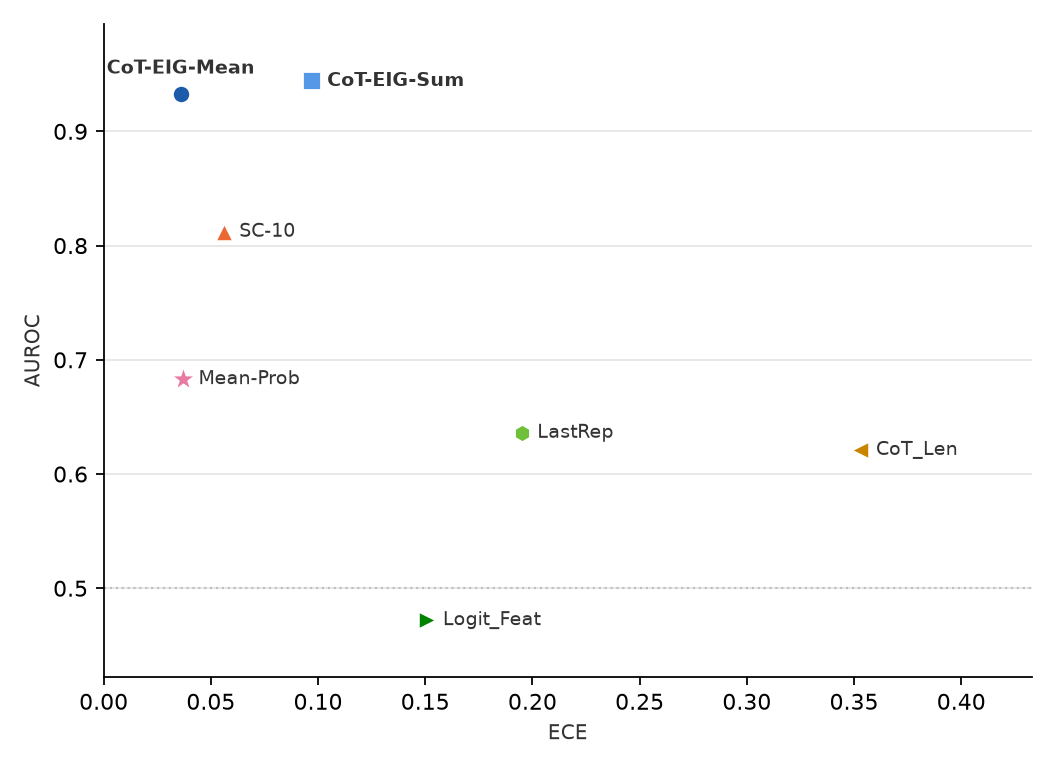
\includegraphics[width=\linewidth]{figures/appendix/roc_against_ece_deepseek_r1_math.png}
        \caption{DeepSeek-R1-Distill-Qwen-7B}
    \end{subfigure}
    \caption{Same as Figure~\ref{fig:auroc_ece_comparison}, with the mathematics domain (GSM8K, MATH500 and AIME) held out.}
    \label{fig:holdout_auroc_ece_math}
\end{figure}

\begin{figure}[h]
    \centering
    \begin{minipage}{0.48\textwidth}
        \centering
        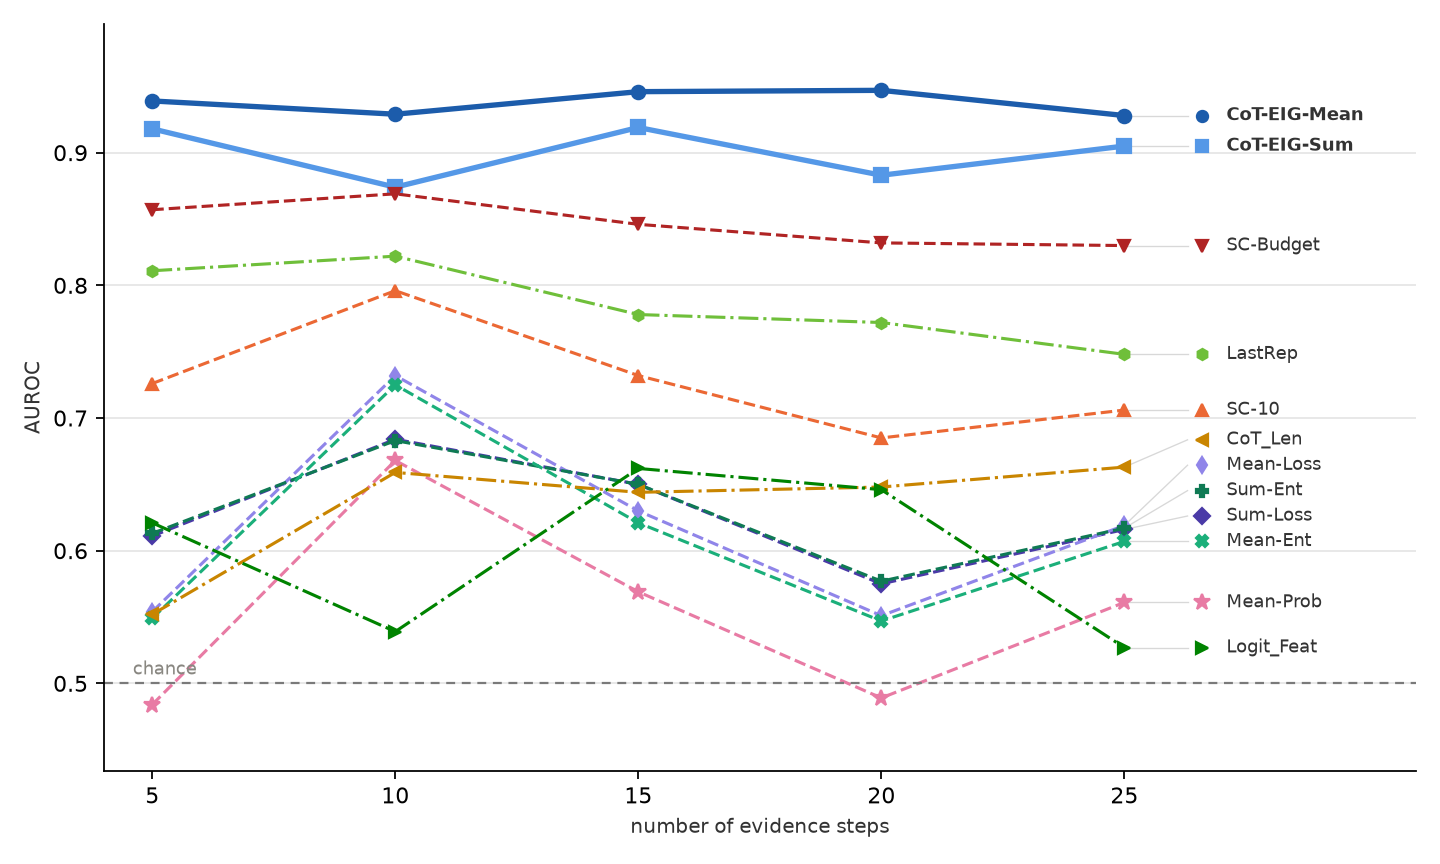
\includegraphics[width=\linewidth]{figures/appendix/roc_by_evidence_count_qwen3_math.png}
        \centerline{(a) Qwen3-8B, AUROC}
    \end{minipage}
    \hfill
    \begin{minipage}{0.48\textwidth}
        \centering
        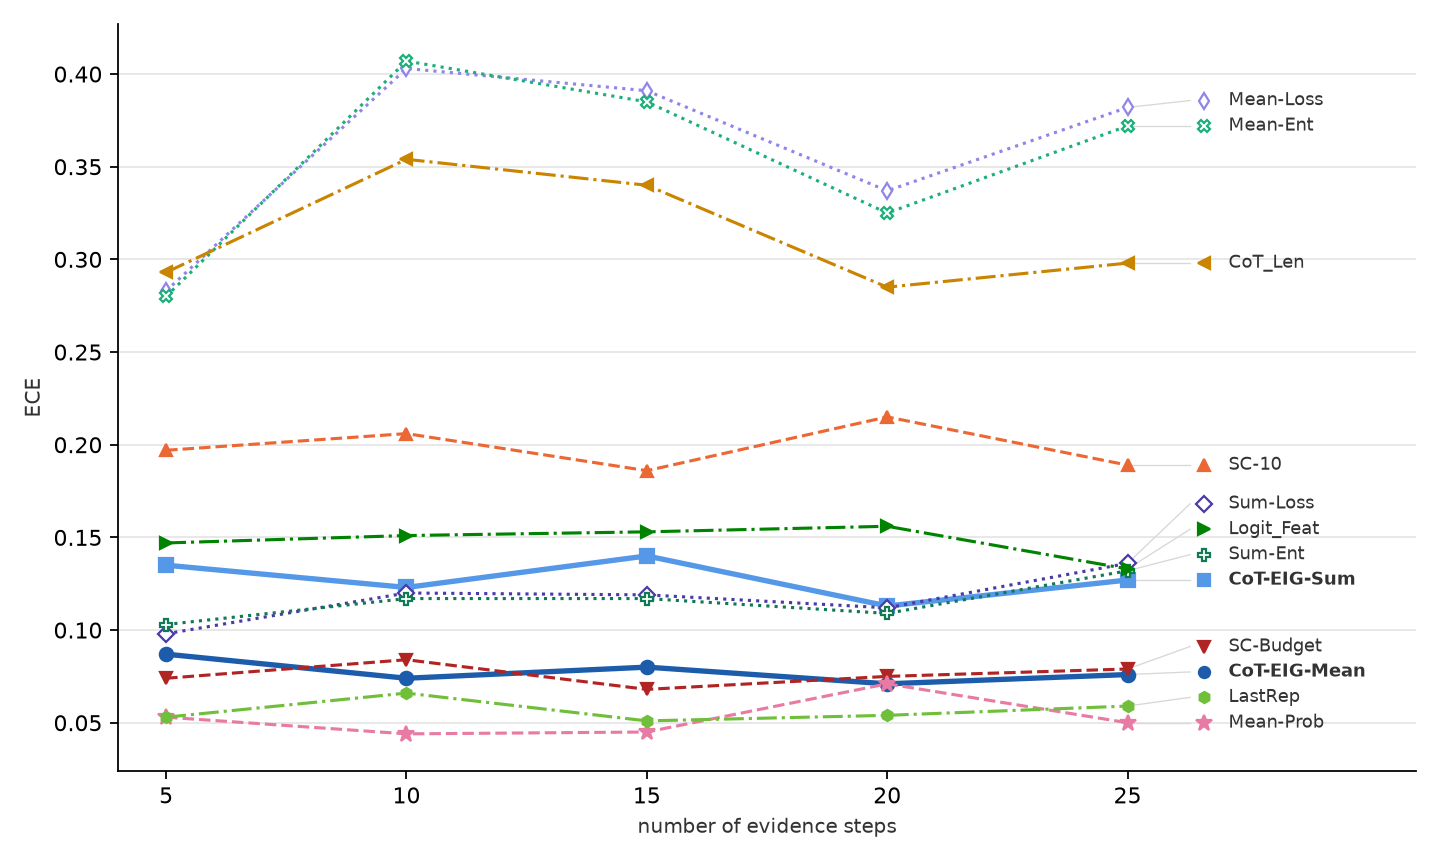
\includegraphics[width=\linewidth]{figures/appendix/ece_by_evidence_count_qwen3_math.png}
        \centerline{(b) Qwen3-8B, ECE}
    \end{minipage}

    \vspace{0.5em}

    \begin{minipage}{0.48\textwidth}
        \centering
        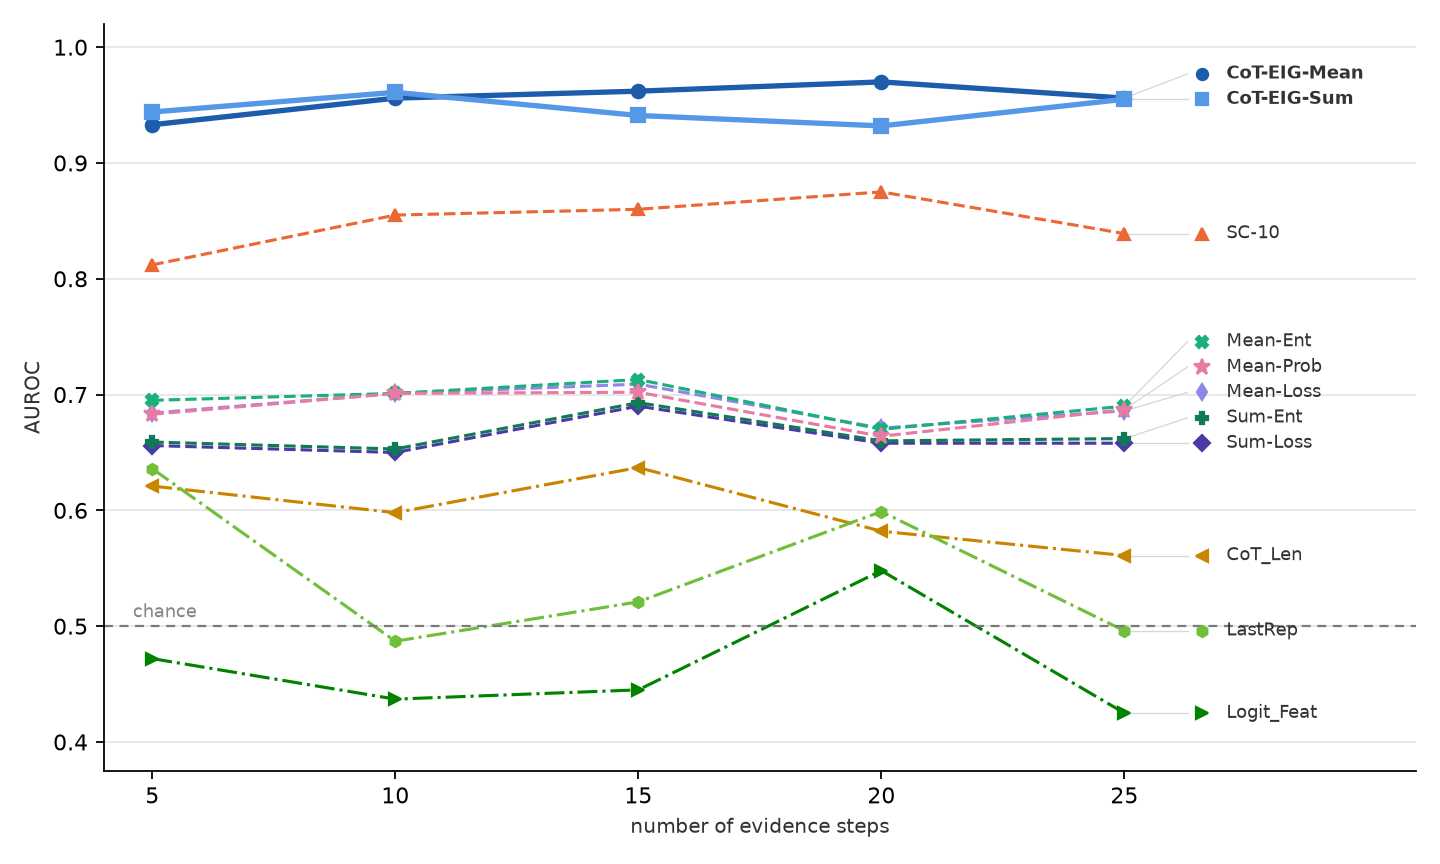
\includegraphics[width=\linewidth]{figures/appendix/roc_by_evidence_count_deepseek_r1_math.png}
        \centerline{(c) DeepSeek-R1-Distill-Qwen-7B, AUROC}
    \end{minipage}
    \hfill
    \begin{minipage}{0.48\textwidth}
        \centering
        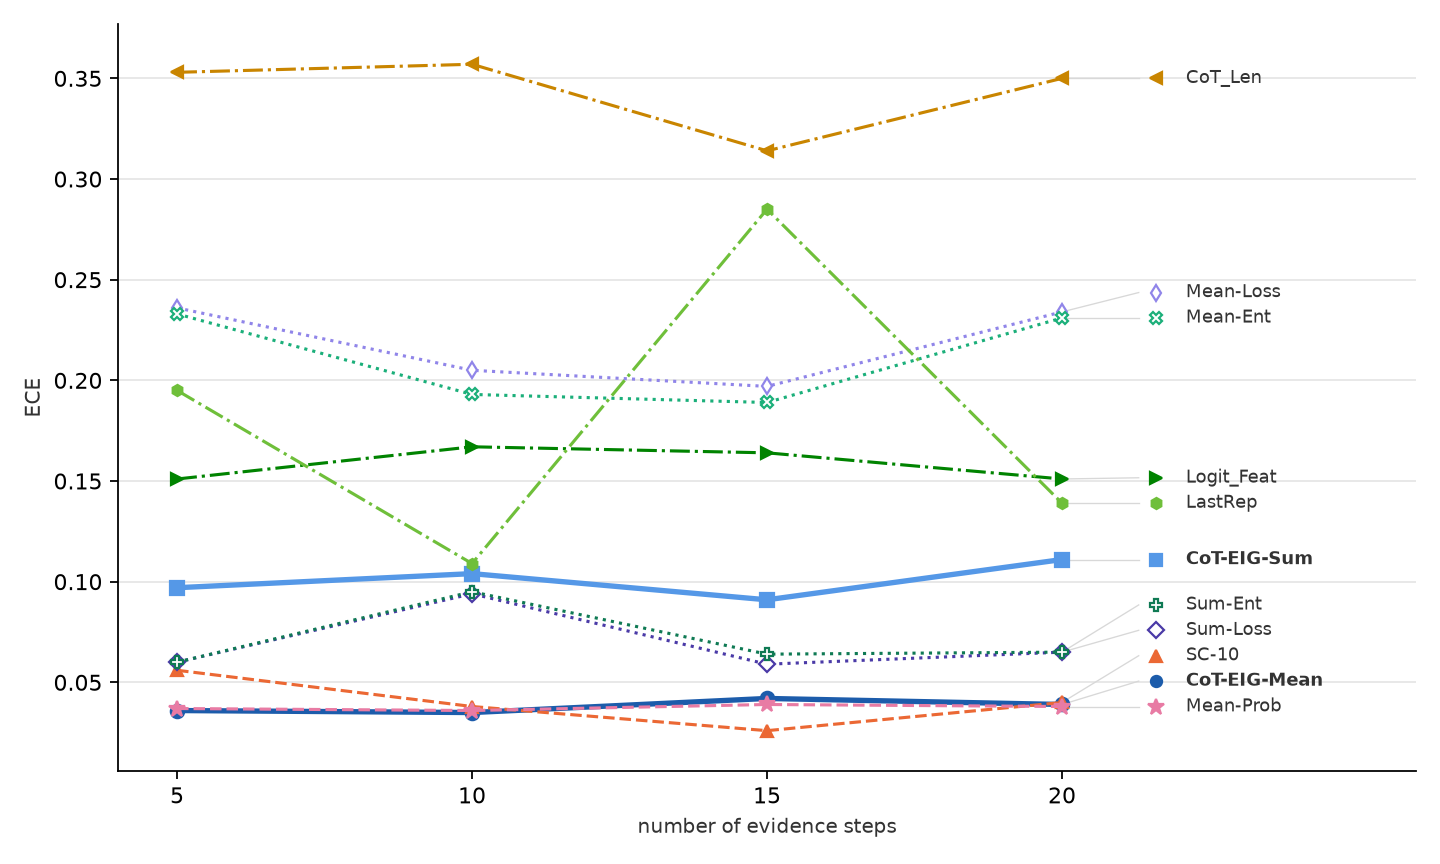
\includegraphics[width=\linewidth]{figures/appendix/ece_by_evidence_count_deepseek_r1_math.png}
        \centerline{(d) DeepSeek-R1-Distill-Qwen-7B, ECE}
    \end{minipage}
    \caption{Same as Figure~\ref{fig:evidence_ablation_models}, with the mathematics domain (GSM8K, MATH500 and AIME) held out.}
    \label{fig:holdout_evidence_math}

    \vspace{1.5em}

    % Side by side rather than stacked, so this figure fits on the page above with it.
    \begin{subfigure}{0.48\linewidth}
        \centering
        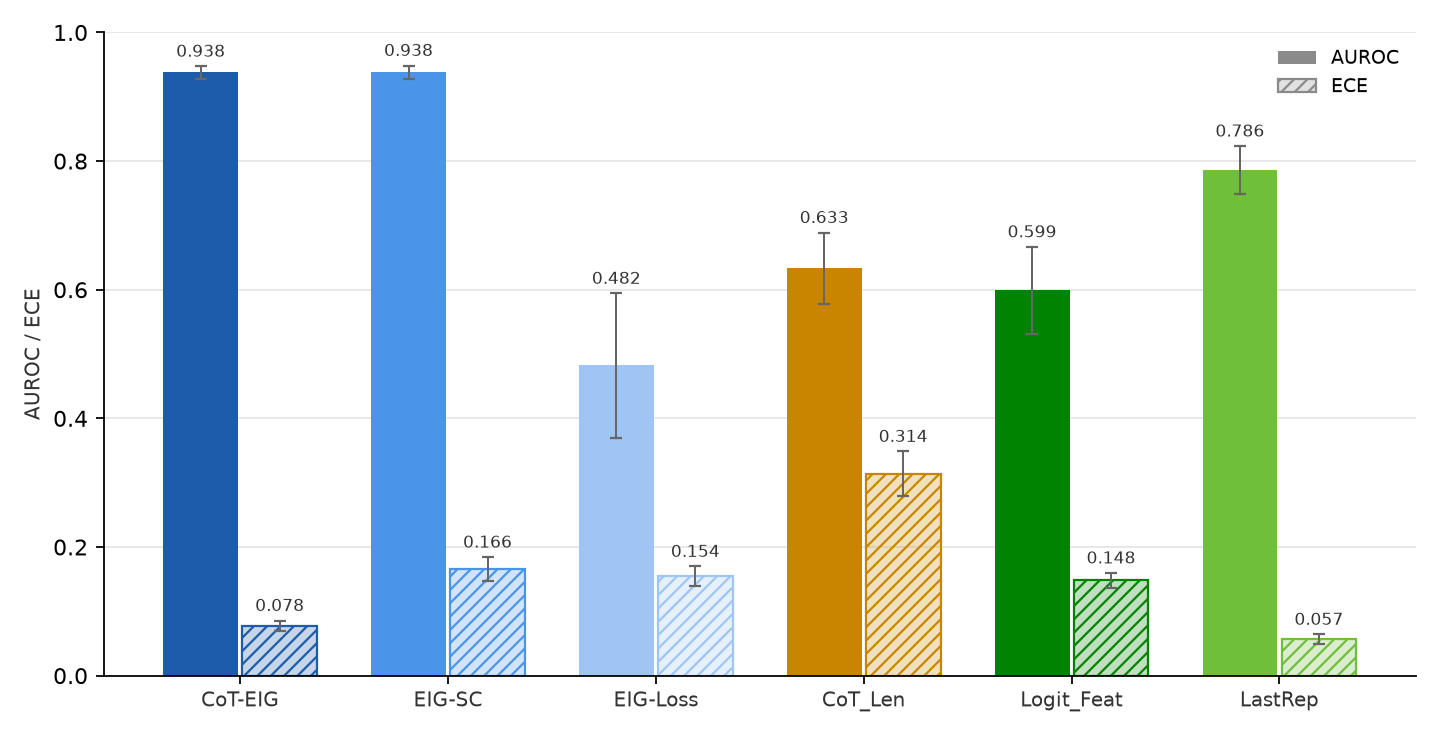
\includegraphics[width=\linewidth]{figures/appendix/roc_ece_by_feature_set_qwen3_math.png}
        \caption{Qwen3-8B}
    \end{subfigure}
    \hfill
    \begin{subfigure}{0.48\linewidth}
        \centering
        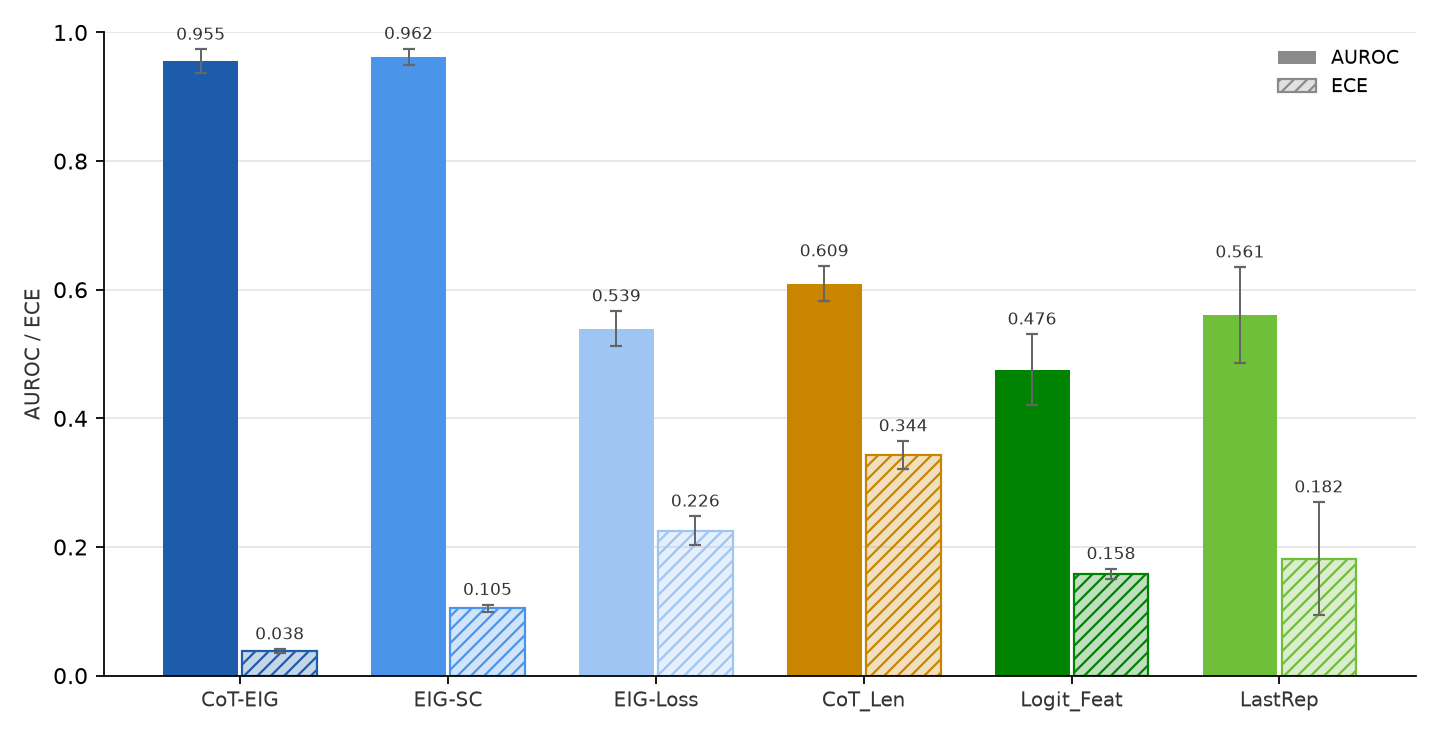
\includegraphics[width=\linewidth]{figures/appendix/roc_ece_by_feature_set_deepseek_r1_math.png}
        \caption{DeepSeek-R1-Distill-Qwen-7B}
    \end{subfigure}
    \caption{Same as Figure~\ref{fig:feature_ablation}, with the mathematics domain (GSM8K, MATH500 and AIME) held out.}
    \label{fig:holdout_feature_ablation_math}
\end{figure}

\clearpage

\subsection{GPQA}
\label{subsec:appendix_holdout_gpqa}

\begin{table}[h]
    \centering
    \caption{Same as Table~\ref{tab:confidence_results}, with GPQA held out.}
    \label{tab:holdout_gpqa}
    \resizebox{\linewidth}{!}{%
    \begin{tabular}{lcc|cc}
        \toprule
        \multirow{2}{*}{Method} &
        \multicolumn{2}{c|}{Qwen3-8B} &
        \multicolumn{2}{c}{DeepSeek-R1-Distill-Qwen-7B} \\
        & AUROC $\uparrow$ & ECE $\downarrow$
        & AUROC $\uparrow$ & ECE $\downarrow$ \\
        \midrule
        \multicolumn{5}{c}{\textit{Token-level baselines}} \\
        \midrule
        Mean-Ent & $0.58 \pm 0.04$ & $\mathbf{0.14 \pm 0.03}$ & $0.56 \pm 0.05$ & $0.17 \pm 0.03$ \\
        Sum-Ent & $0.53 \pm 0.04$ & $0.43 \pm 0.04$ & $0.60 \pm 0.05$ & $0.23 \pm 0.03$ \\
        Mean-Loss & $0.57 \pm 0.04$ & $0.16 \pm 0.03$ & $0.55 \pm 0.05$ & $0.17 \pm 0.04$ \\
        Sum-Loss & $0.53 \pm 0.04$ & $0.43 \pm 0.04$ & $0.60 \pm 0.05$ & $0.22 \pm 0.03$ \\
        Mean-Prob & $0.56 \pm 0.04$ & $0.38 \pm 0.04$ & $0.56 \pm 0.05$ & $0.34 \pm 0.04$ \\
        \midrule
        \multicolumn{5}{c}{\textit{Representation-based baseline}} \\
        \midrule
        LastRep & $0.57 \pm 0.04$ & $0.33 \pm 0.03$ & $0.65 \pm 0.04$ & $0.28 \pm 0.04$ \\
        \midrule
        \multicolumn{5}{c}{\textit{Self-consistency baselines}} \\
        \midrule
        SC-10 & $0.61 \pm 0.04$ & $0.31 \pm 0.05$ & $0.73 \pm 0.04$ & $0.20 \pm 0.03$ \\
        SC-Budget & $0.64 \pm 0.04$ & $0.29 \pm 0.04$ & --- & --- \\
        \midrule
        \multicolumn{5}{c}{\textit{Proposed method}} \\
        \midrule
        CoT-EIG-Mean & $\mathbf{0.72 \pm 0.04}$ & $0.25 \pm 0.03$ & $\mathbf{0.79 \pm 0.03}$ & $\mathbf{0.14 \pm 0.03}$ \\
        CoT-EIG-Sum & $0.67 \pm 0.04$ & $0.25 \pm 0.04$ & $\mathbf{0.79 \pm 0.03}$ & $0.15 \pm 0.03$ \\
        \bottomrule
    \end{tabular}%
    }
\end{table}


\begin{figure}[h]
    \centering
    \begin{subfigure}{0.48\linewidth}
        \centering
        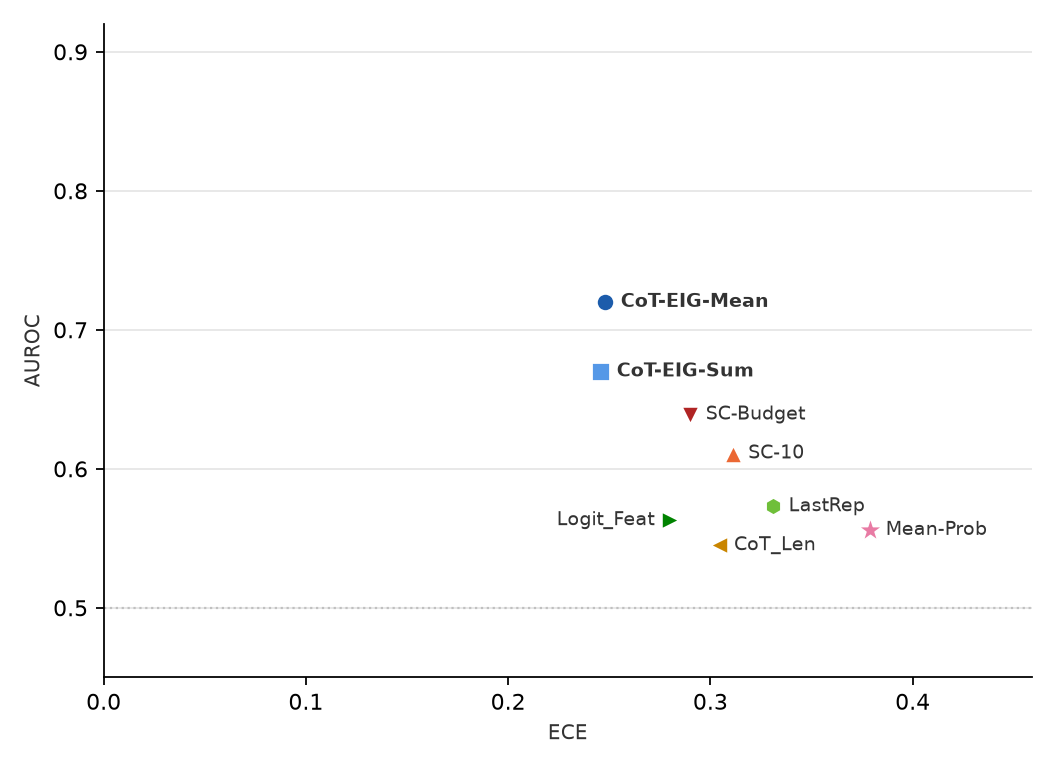
\includegraphics[width=\linewidth]{figures/appendix/roc_against_ece_qwen3_gpqa.png}
        \caption{Qwen3-8B}
    \end{subfigure}
    \hfill
    \begin{subfigure}{0.48\linewidth}
        \centering
        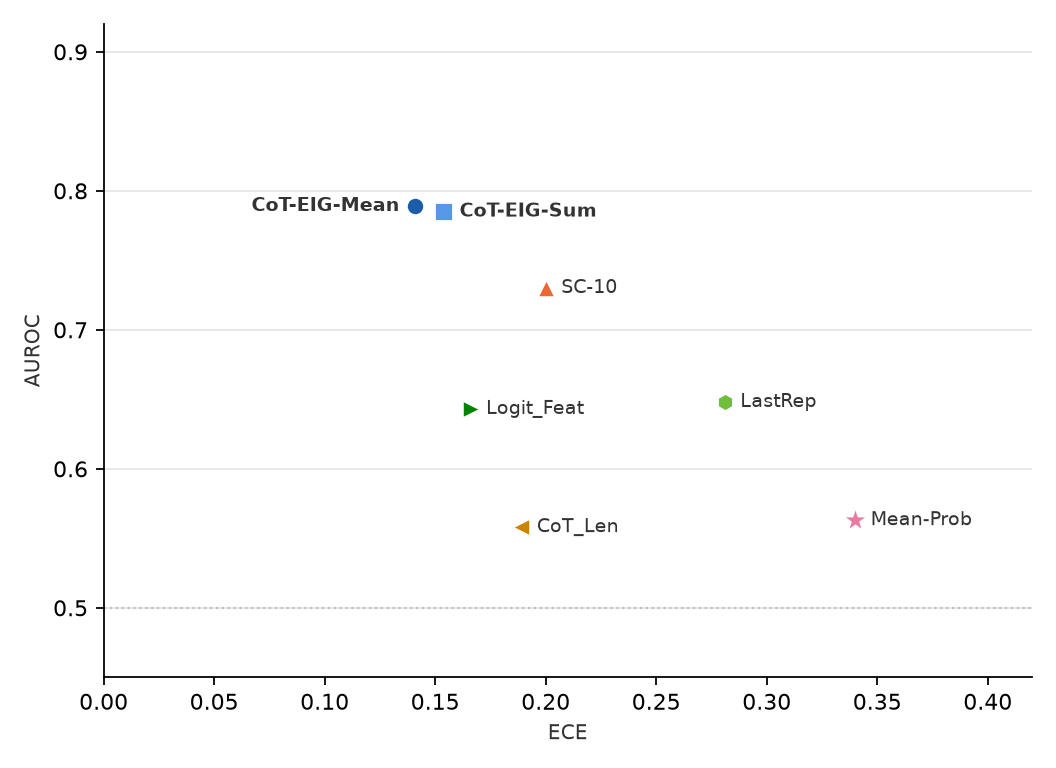
\includegraphics[width=\linewidth]{figures/appendix/roc_against_ece_deepseek_r1_gpqa.png}
        \caption{DeepSeek-R1-Distill-Qwen-7B}
    \end{subfigure}
    \caption{Same as Figure~\ref{fig:auroc_ece_comparison}, with GPQA held out.}
    \label{fig:holdout_auroc_ece_gpqa}
\end{figure}

\begin{figure}[h]
    \centering
    \begin{minipage}{0.48\textwidth}
        \centering
        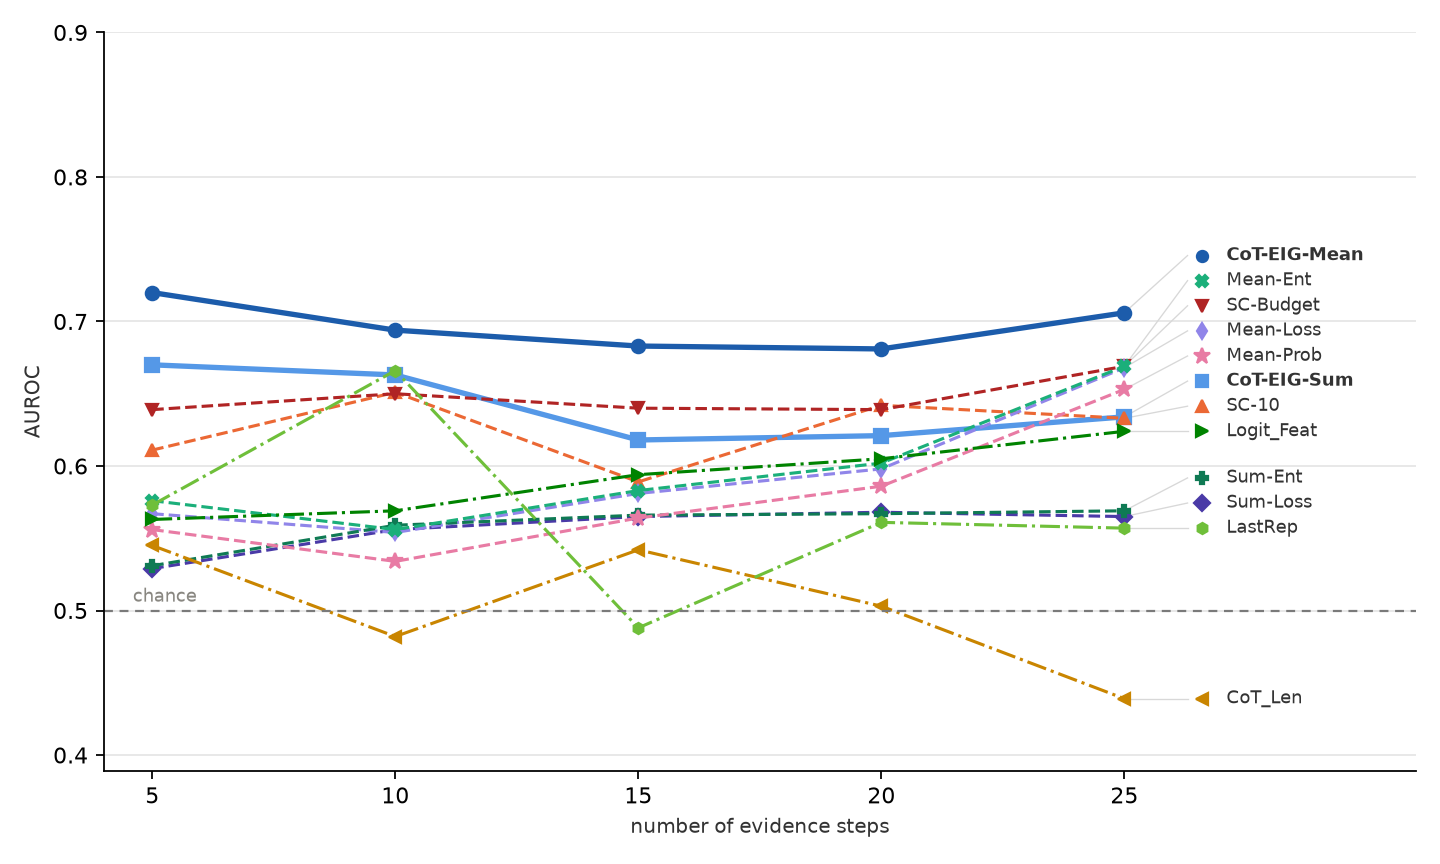
\includegraphics[width=\linewidth]{figures/appendix/roc_by_evidence_count_qwen3_gpqa.png}
        \centerline{(a) Qwen3-8B, AUROC}
    \end{minipage}
    \hfill
    \begin{minipage}{0.48\textwidth}
        \centering
        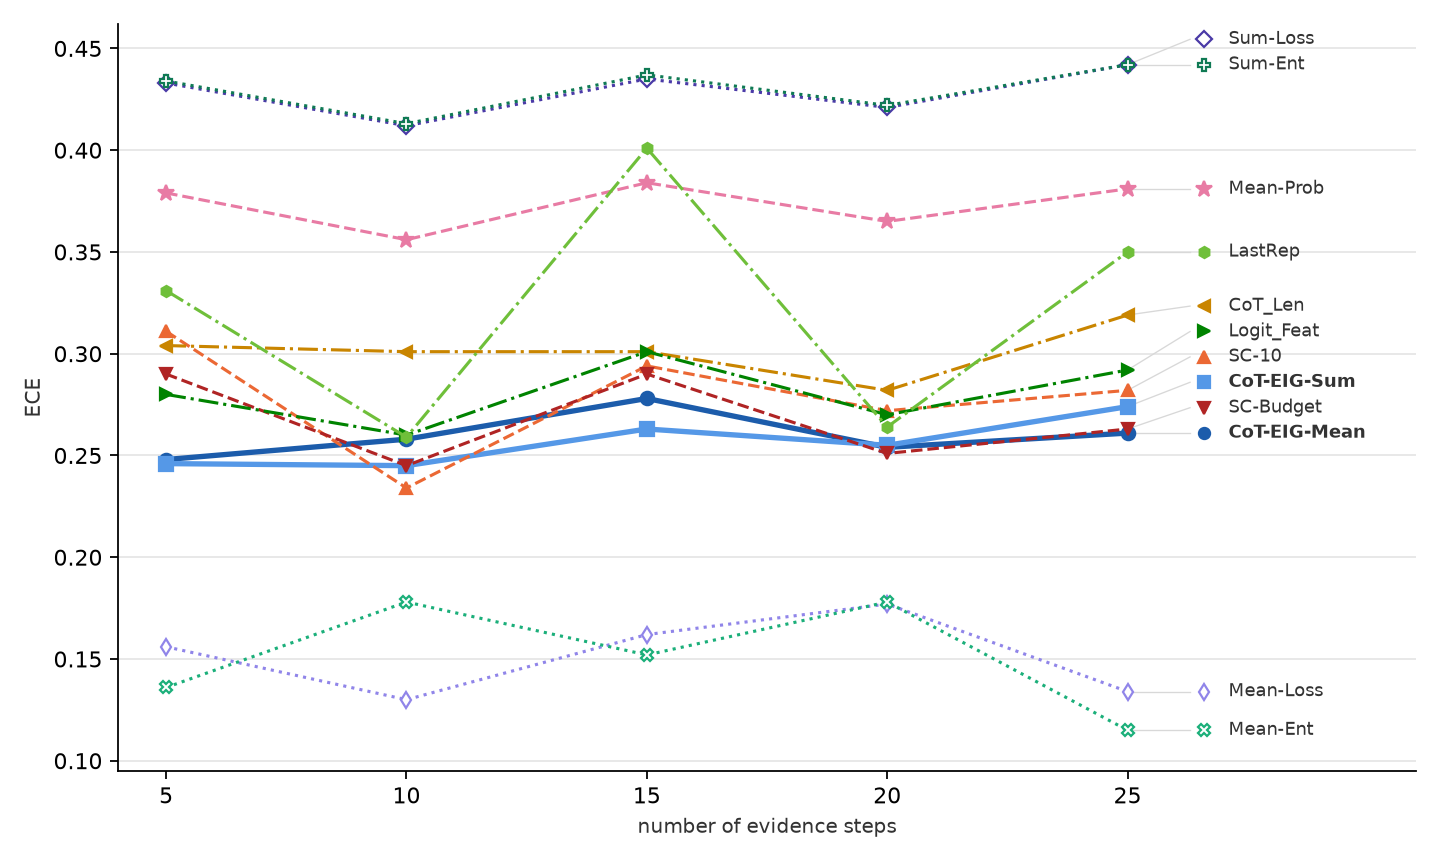
\includegraphics[width=\linewidth]{figures/appendix/ece_by_evidence_count_qwen3_gpqa.png}
        \centerline{(b) Qwen3-8B, ECE}
    \end{minipage}

    \vspace{0.5em}

    \begin{minipage}{0.48\textwidth}
        \centering
        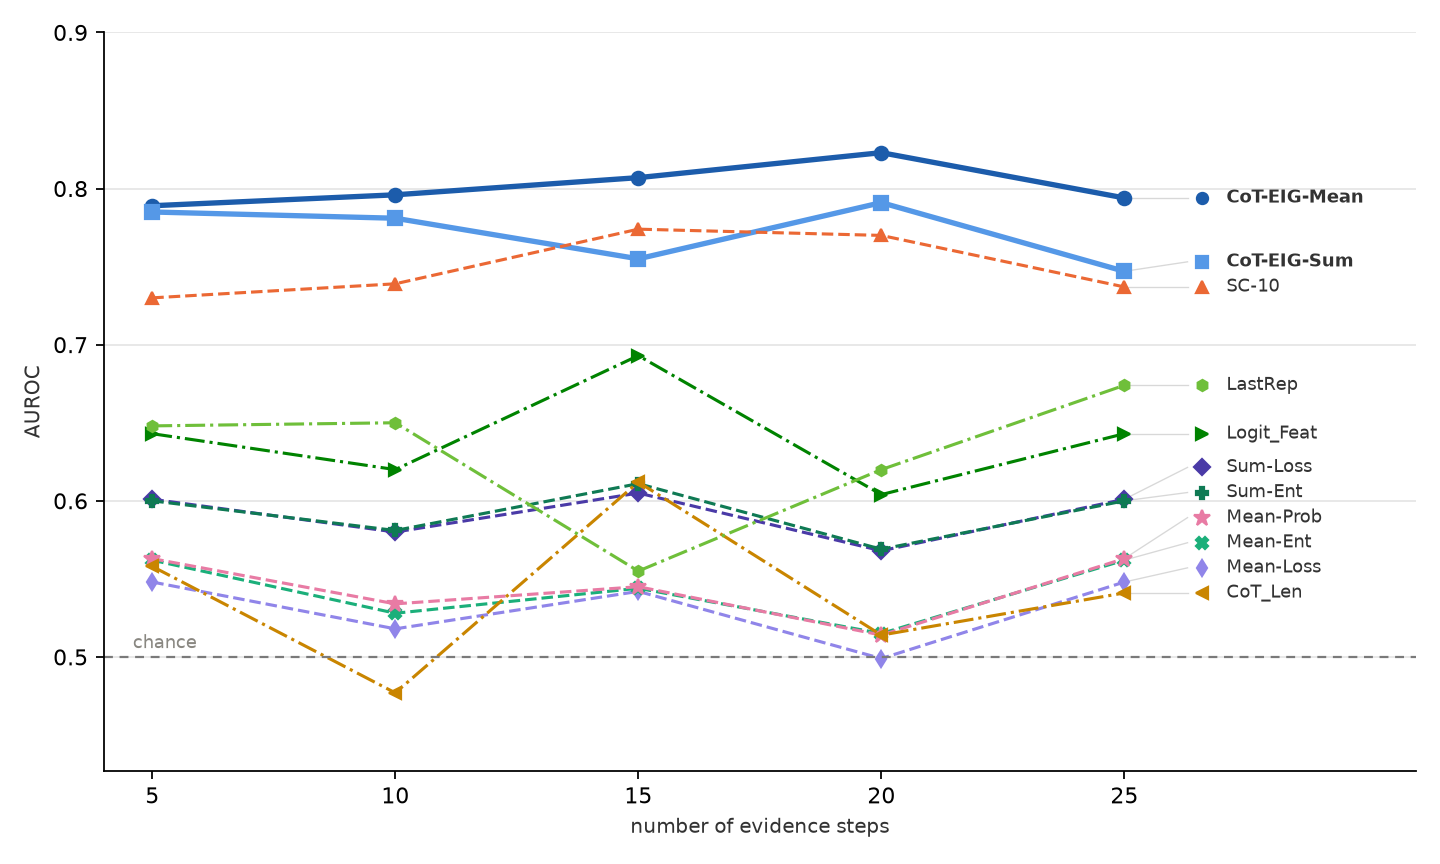
\includegraphics[width=\linewidth]{figures/appendix/roc_by_evidence_count_deepseek_r1_gpqa.png}
        \centerline{(c) DeepSeek-R1-Distill-Qwen-7B, AUROC}
    \end{minipage}
    \hfill
    \begin{minipage}{0.48\textwidth}
        \centering
        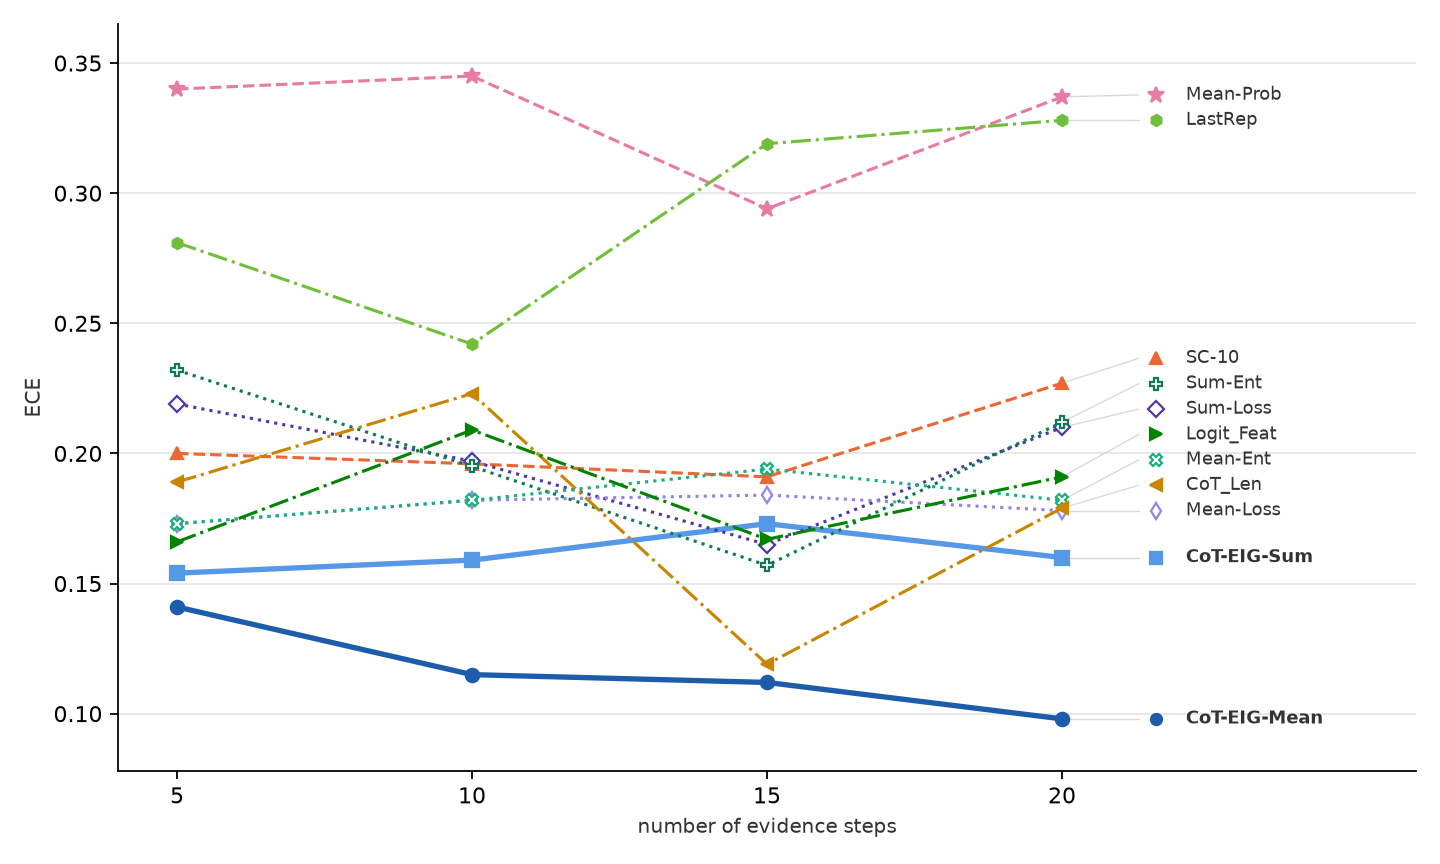
\includegraphics[width=\linewidth]{figures/appendix/ece_by_evidence_count_deepseek_r1_gpqa.png}
        \centerline{(d) DeepSeek-R1-Distill-Qwen-7B, ECE}
    \end{minipage}
    \caption{Same as Figure~\ref{fig:evidence_ablation_models}, with GPQA held out.}
    \label{fig:holdout_evidence_gpqa}

    \vspace{1.5em}

    % Side by side rather than stacked, so this figure fits on the page above with it.
    \begin{subfigure}{0.48\linewidth}
        \centering
        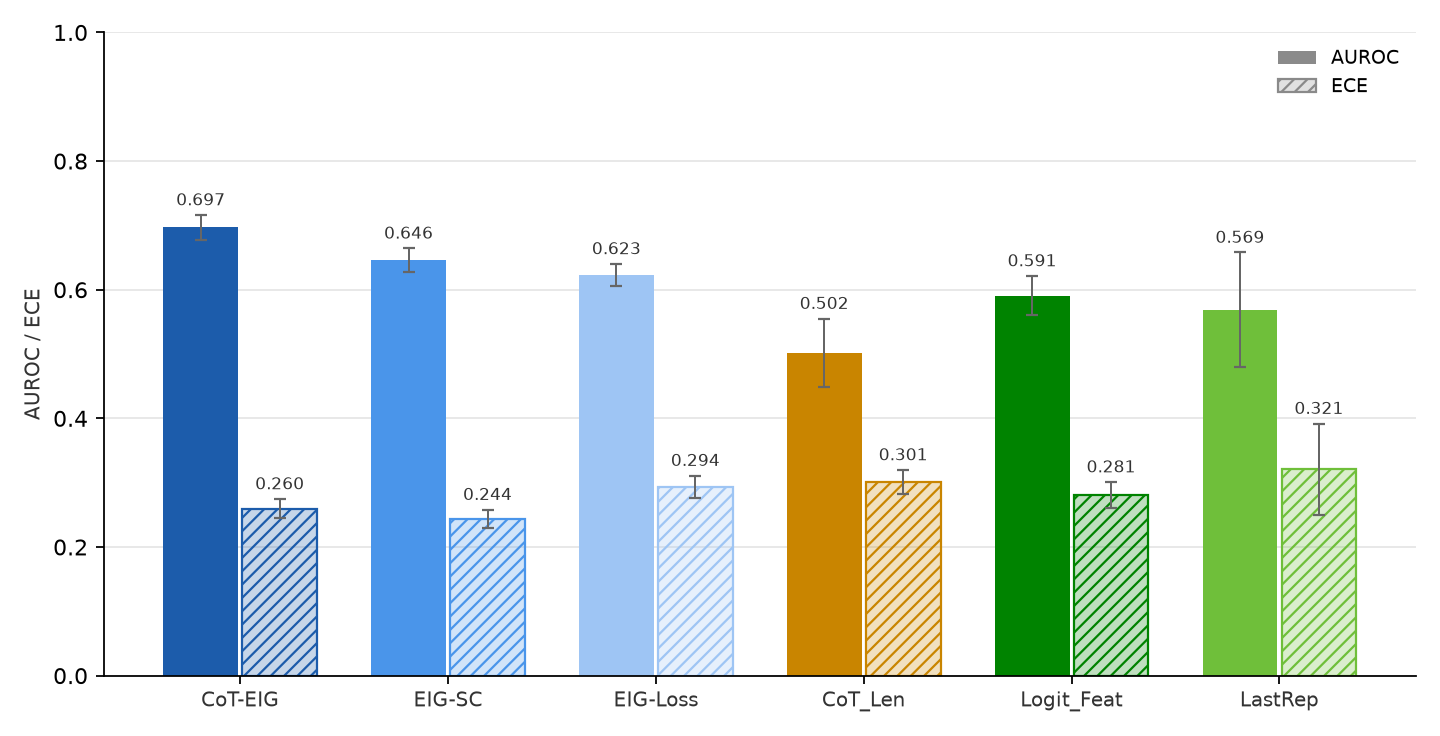
\includegraphics[width=\linewidth]{figures/appendix/roc_ece_by_feature_set_qwen3_gpqa.png}
        \caption{Qwen3-8B}
    \end{subfigure}
    \hfill
    \begin{subfigure}{0.48\linewidth}
        \centering
        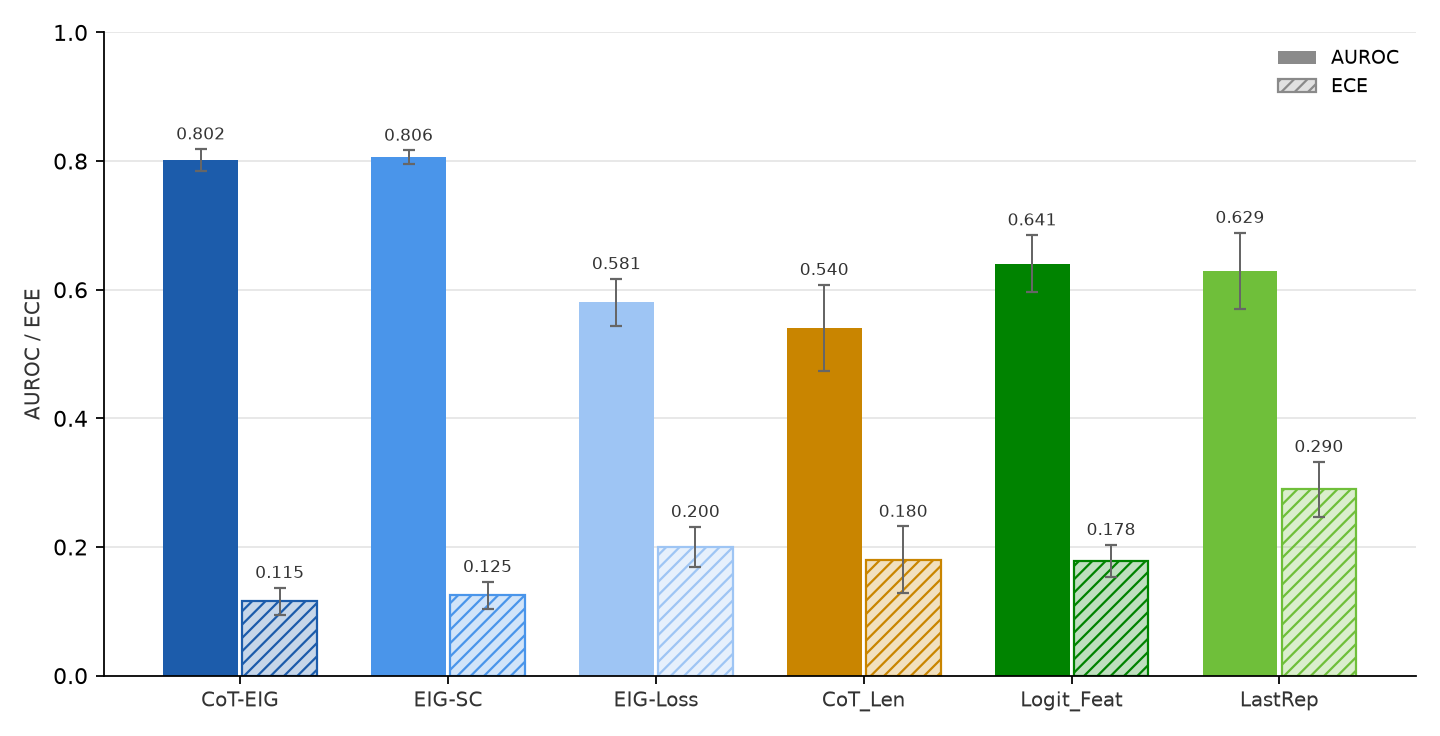
\includegraphics[width=\linewidth]{figures/appendix/roc_ece_by_feature_set_deepseek_r1_gpqa.png}
        \caption{DeepSeek-R1-Distill-Qwen-7B}
    \end{subfigure}
    \caption{Same as Figure~\ref{fig:feature_ablation}, with GPQA held out.}
    \label{fig:holdout_feature_ablation_gpqa}
\end{figure}

\clearpage

\subsection{TruthfulQA}
\label{subsec:appendix_holdout_truthfulqa}

\begin{table}[h]
    \centering
    \caption{Same as Table~\ref{tab:confidence_results}, with TruthfulQA held out.}
    \label{tab:holdout_truthfulqa}
    \resizebox{\linewidth}{!}{%
    \begin{tabular}{lcc|cc}
        \toprule
        \multirow{2}{*}{Method} &
        \multicolumn{2}{c|}{Qwen3-8B} &
        \multicolumn{2}{c}{DeepSeek-R1-Distill-Qwen-7B} \\
        & AUROC $\uparrow$ & ECE $\downarrow$
        & AUROC $\uparrow$ & ECE $\downarrow$ \\
        \midrule
        \multicolumn{5}{c}{\textit{Token-level baselines}} \\
        \midrule
        Mean-Ent & $0.66 \pm 0.03$ & $0.25 \pm 0.03$ & $0.53 \pm 0.03$ & $0.12 \pm 0.03$ \\
        Sum-Ent & $0.65 \pm 0.03$ & $0.15 \pm 0.02$ & $0.55 \pm 0.03$ & $0.41 \pm 0.03$ \\
        Mean-Loss & $0.68 \pm 0.03$ & $0.26 \pm 0.02$ & $0.53 \pm 0.03$ & $0.12 \pm 0.03$ \\
        Sum-Loss & $0.66 \pm 0.03$ & $0.15 \pm 0.02$ & $0.55 \pm 0.03$ & $0.41 \pm 0.03$ \\
        Mean-Prob & $0.65 \pm 0.03$ & $0.12 \pm 0.02$ & $0.53 \pm 0.03$ & $0.28 \pm 0.03$ \\
        \midrule
        \multicolumn{5}{c}{\textit{Representation-based baseline}} \\
        \midrule
        LastRep & $0.44 \pm 0.04$ & $0.45 \pm 0.03$ & $0.48 \pm 0.03$ & $0.42 \pm 0.03$ \\
        \midrule
        \multicolumn{5}{c}{\textit{Self-consistency baselines}} \\
        \midrule
        SC-10 & $0.72 \pm 0.03$ & $0.11 \pm 0.02$ & $0.59 \pm 0.03$ & $0.24 \pm 0.03$ \\
        SC-Budget & $0.84 \pm 0.02$ & $0.13 \pm 0.02$ & --- & --- \\
        \midrule
        \multicolumn{5}{c}{\textit{Proposed method}} \\
        \midrule
        CoT-EIG-Mean & $\mathbf{0.87 \pm 0.02}$ & $\mathbf{0.07 \pm 0.02}$ & $0.75 \pm 0.03$ & $\mathbf{0.10 \pm 0.02}$ \\
        CoT-EIG-Sum & $0.84 \pm 0.02$ & $\mathbf{0.07 \pm 0.02}$ & $\mathbf{0.76 \pm 0.03}$ & $0.17 \pm 0.02$ \\
        \bottomrule
    \end{tabular}%
    }
\end{table}


\begin{figure}[h]
    \centering
    \begin{subfigure}{0.48\linewidth}
        \centering
        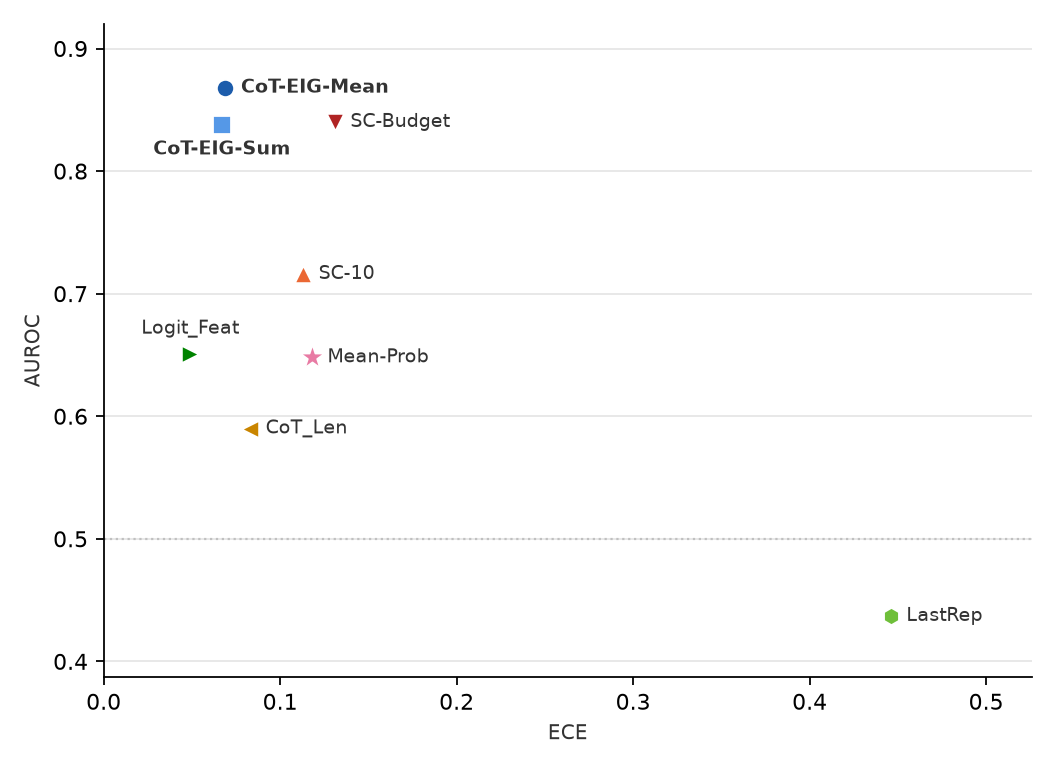
\includegraphics[width=\linewidth]{figures/appendix/roc_against_ece_qwen3_truthfulqa.png}
        \caption{Qwen3-8B}
    \end{subfigure}
    \hfill
    \begin{subfigure}{0.48\linewidth}
        \centering
        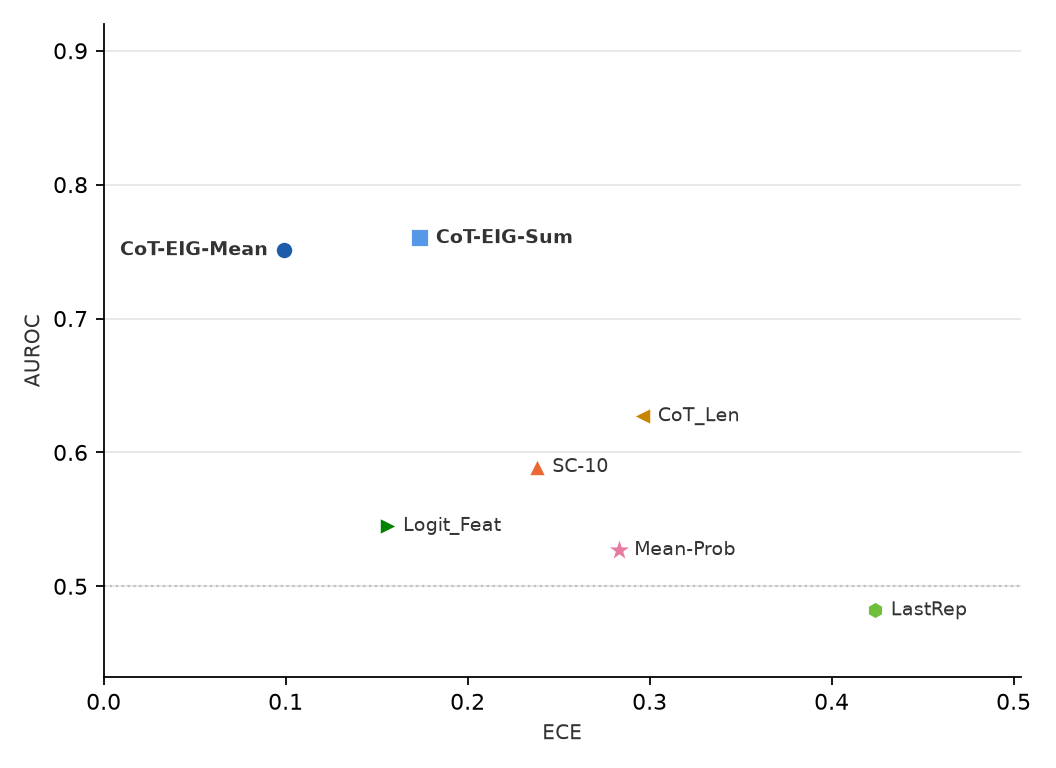
\includegraphics[width=\linewidth]{figures/appendix/roc_against_ece_deepseek_r1_truthfulqa.png}
        \caption{DeepSeek-R1-Distill-Qwen-7B}
    \end{subfigure}
    \caption{Same as Figure~\ref{fig:auroc_ece_comparison}, with TruthfulQA held out.}
    \label{fig:holdout_auroc_ece_truthfulqa}
\end{figure}

\begin{figure}[h]
    \centering
    \begin{minipage}{0.48\textwidth}
        \centering
        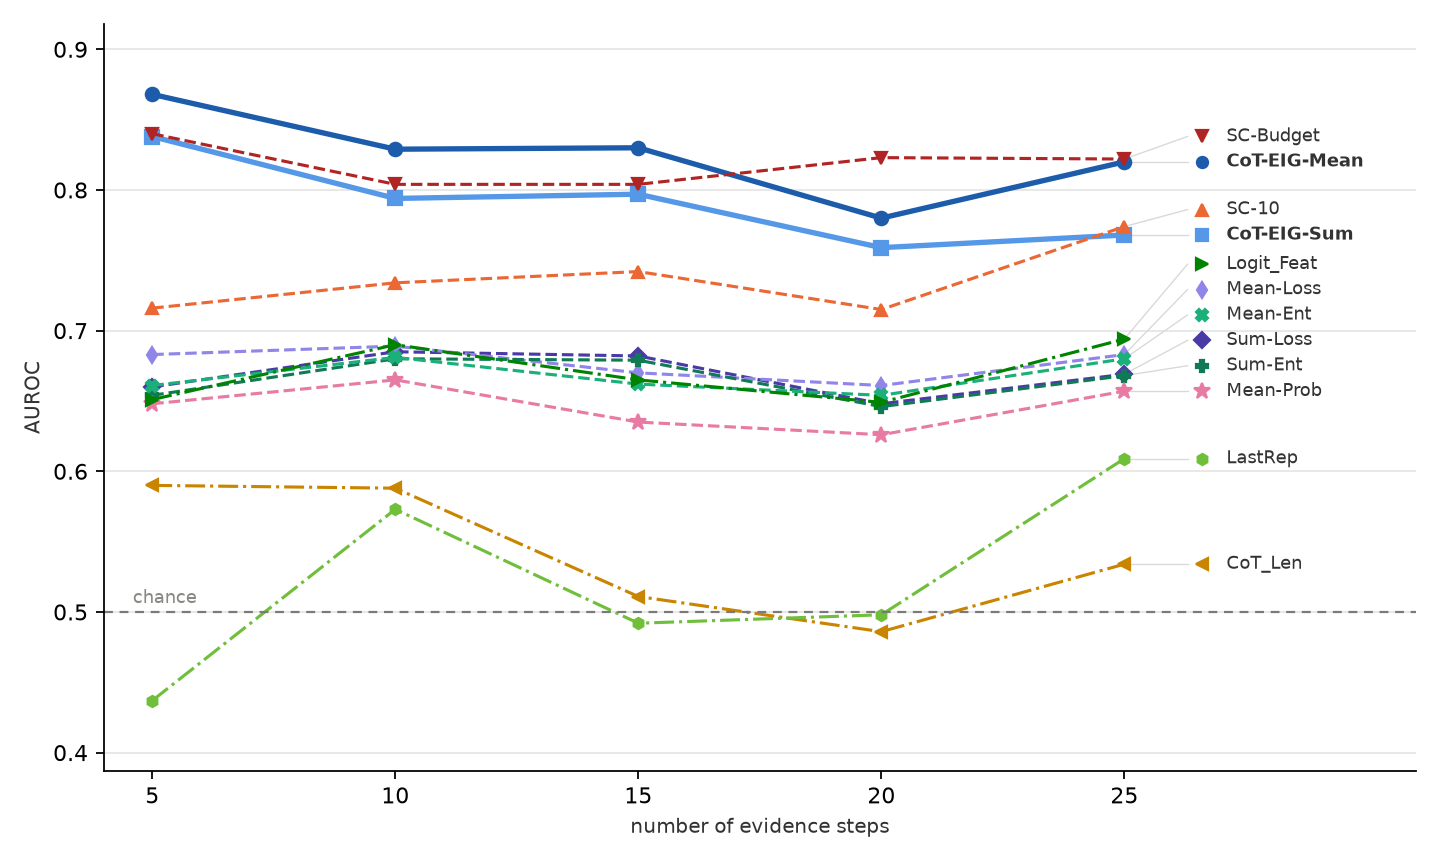
\includegraphics[width=\linewidth]{figures/appendix/roc_by_evidence_count_qwen3_truthfulqa.png}
        \centerline{(a) Qwen3-8B, AUROC}
    \end{minipage}
    \hfill
    \begin{minipage}{0.48\textwidth}
        \centering
        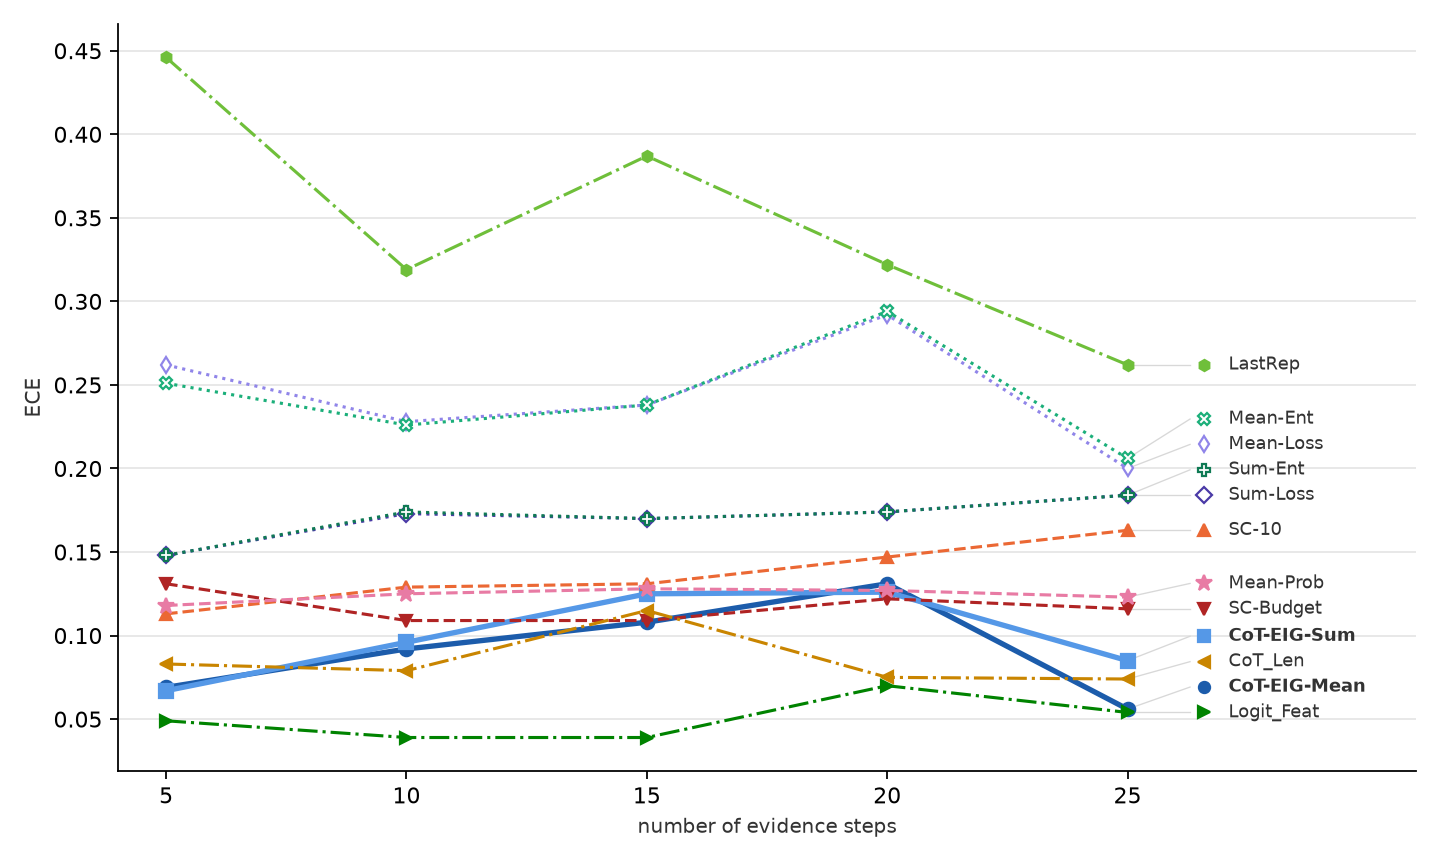
\includegraphics[width=\linewidth]{figures/appendix/ece_by_evidence_count_qwen3_truthfulqa.png}
        \centerline{(b) Qwen3-8B, ECE}
    \end{minipage}

    \vspace{0.5em}

    \begin{minipage}{0.48\textwidth}
        \centering
        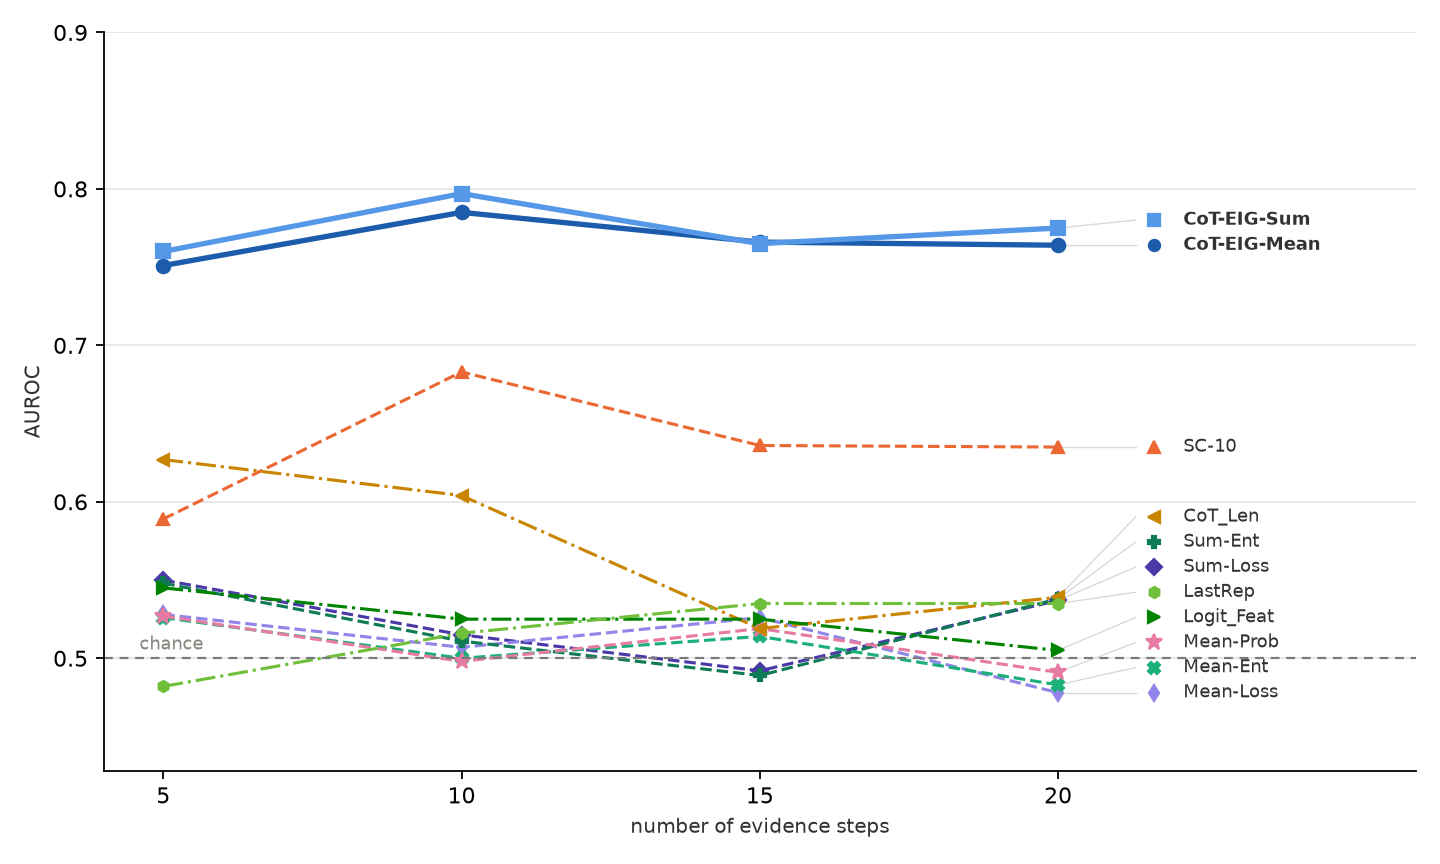
\includegraphics[width=\linewidth]{figures/appendix/roc_by_evidence_count_deepseek_r1_truthfulqa.png}
        \centerline{(c) DeepSeek-R1-Distill-Qwen-7B, AUROC}
    \end{minipage}
    \hfill
    \begin{minipage}{0.48\textwidth}
        \centering
        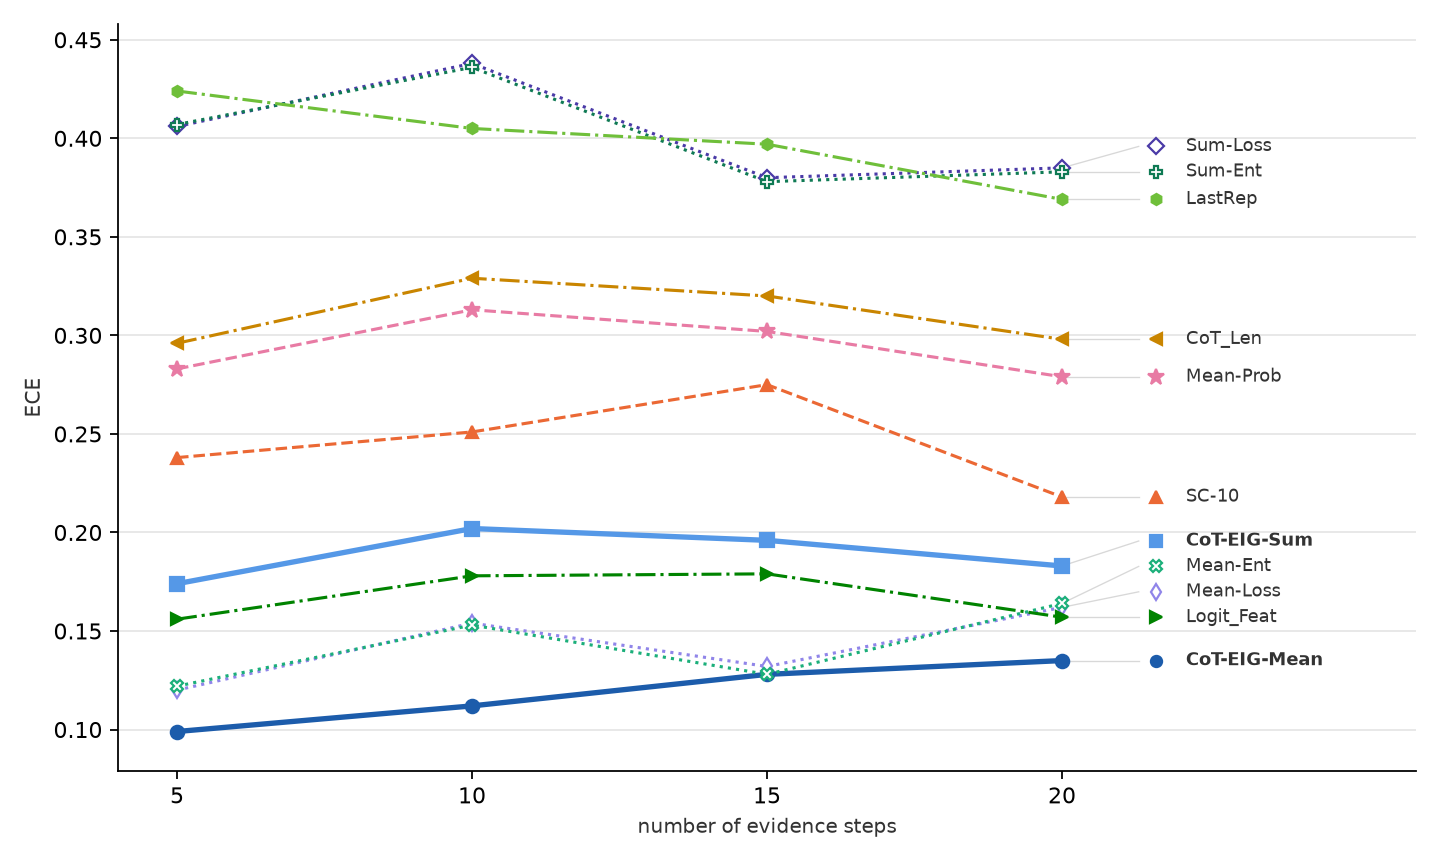
\includegraphics[width=\linewidth]{figures/appendix/ece_by_evidence_count_deepseek_r1_truthfulqa.png}
        \centerline{(d) DeepSeek-R1-Distill-Qwen-7B, ECE}
    \end{minipage}
    \caption{Same as Figure~\ref{fig:evidence_ablation_models}, with TruthfulQA held out.}
    \label{fig:holdout_evidence_truthfulqa}

    \vspace{1.5em}

    % Side by side rather than stacked, so this figure fits on the page above with it.
    \begin{subfigure}{0.48\linewidth}
        \centering
        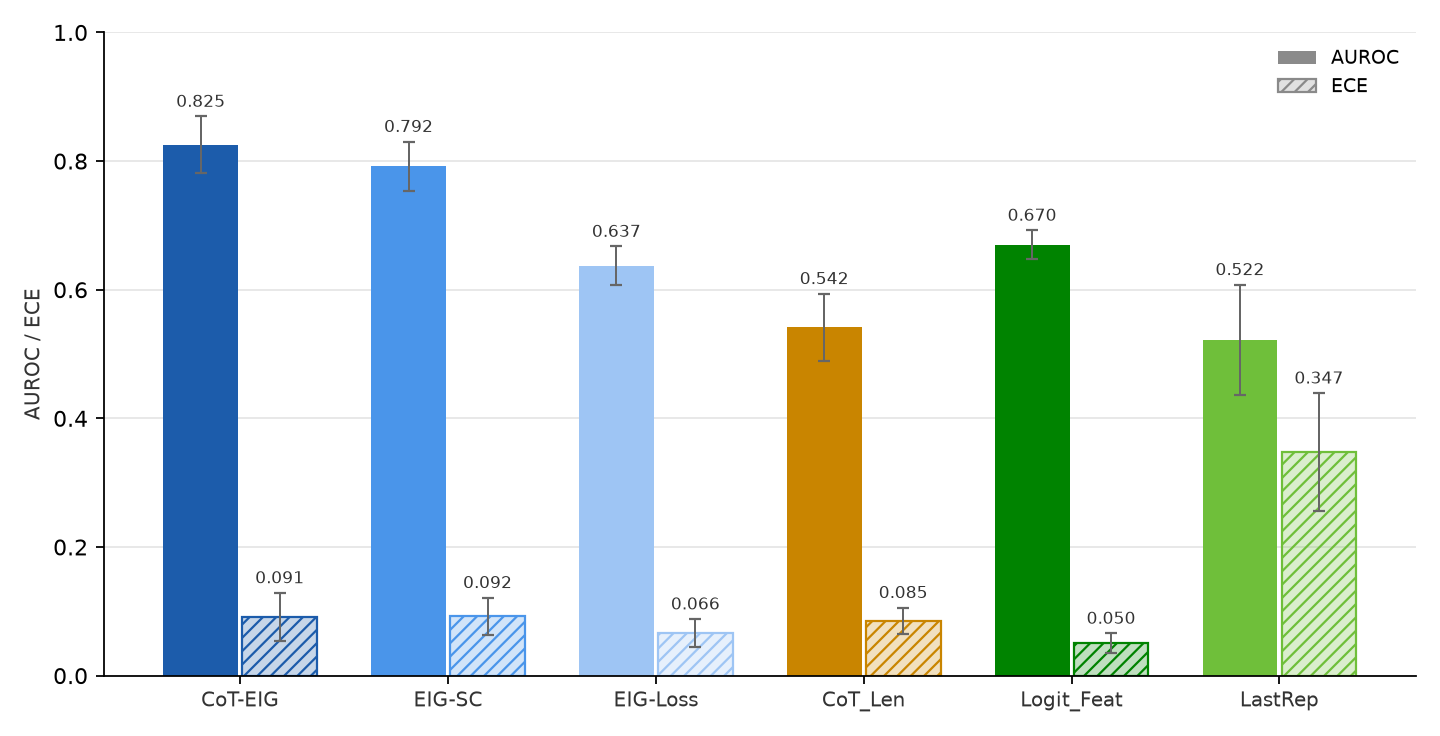
\includegraphics[width=\linewidth]{figures/appendix/roc_ece_by_feature_set_qwen3_truthfulqa.png}
        \caption{Qwen3-8B}
    \end{subfigure}
    \hfill
    \begin{subfigure}{0.48\linewidth}
        \centering
        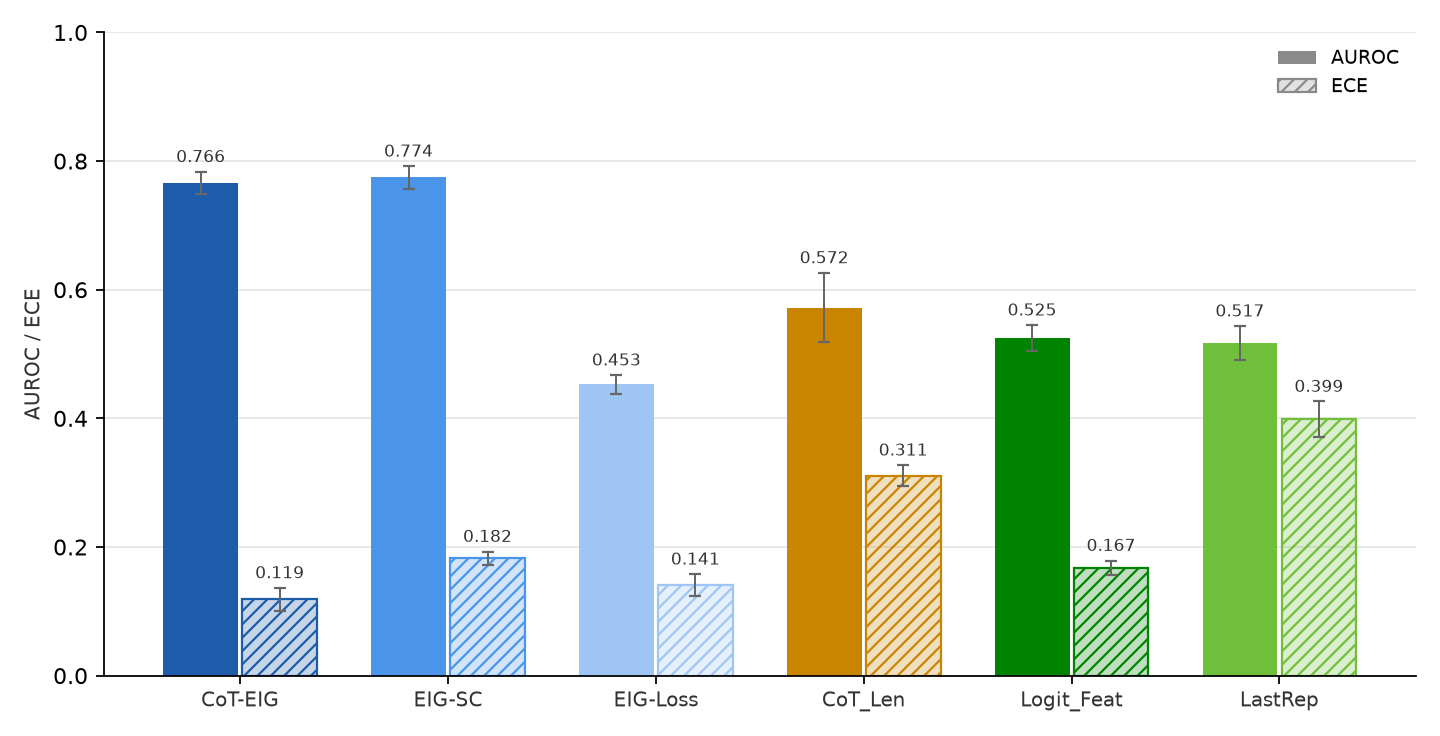
\includegraphics[width=\linewidth]{figures/appendix/roc_ece_by_feature_set_deepseek_r1_truthfulqa.png}
        \caption{DeepSeek-R1-Distill-Qwen-7B}
    \end{subfigure}
    \caption{Same as Figure~\ref{fig:feature_ablation}, with TruthfulQA held out.}
    \label{fig:holdout_feature_ablation_truthfulqa}
\end{figure}


\clearpage

\end{document}
